%======================================================================
% MODULE 3: Real-Time Embedded Systems
%
% Learning Objectives:
% After completing this module, students will be able to:
% - Explain why real-time guarantees are essential for flight control
% - Describe the role of an RTOS in managing concurrent tasks
% - Configure FreeRTOS tasks with appropriate priorities and stack sizes
% - Use task notifications, queues, and timers for inter-task communication
% - Identify and prevent race conditions in concurrent control software
% - Apply synchronization primitives correctly for flight controller tasks
% - Analyze schedulability using RMS and response-time analysis
% - Estimate worst-case execution times for embedded control code
% - Implement fault detection and recovery mechanisms
%======================================================================

\chapter{Real-Time Operating Systems}
\index{RTOS (Real-Time Operating System)}

%----------------------------------------------------------------------
% FIGURE: Module Overview - Quadrotor Software Architecture
%----------------------------------------------------------------------
% Description: High-level view of the software layers in a quadrotor.
%
% Layered diagram (bottom to top):
%   - Hardware layer: MCU, IMU, Motors, Radio
%   - RTOS layer: Scheduler, Memory, Interrupts
%   - Middleware: Sensor drivers, PWM drivers, Communication stack
%   - Application: Control loops, State estimation, Mission logic
%
% Show timing requirements at each level.
% Dimensions: Column width, ~6cm height.
%----------------------------------------------------------------------

\section{Why Real-Time Matters for Quadrotor Control}

In previous modules, we developed the mathematical models for quadrotor dynamics and orientation estimation. Now we face a critical question: \textbf{how do we implement these algorithms on an embedded processor so that they execute reliably and on time?}

This question matters because control theory assumes perfect timing. When we design a controller using discrete-time methods, we assume the controller executes exactly once per sample period $T_s$, computes instantaneously, and outputs immediately. In reality:
\begin{itemize}
    \item Computation takes time---the control law does not execute ``instantaneously''
    \item Multiple tasks compete for the same processor
    \item External events (sensor data, communication) arrive asynchronously
    \item Memory and peripheral access can cause unpredictable delays
\end{itemize}

A Real-Time Operating System (RTOS) provides the infrastructure to manage these complexities systematically.

\subsection{The Multi-Rate Control Problem}

A quadrotor flight controller must run multiple control loops simultaneously, each with different timing requirements:

\begin{center}
\begin{tabular}{lccc}
\toprule
\textbf{Task} & \textbf{Rate} & \textbf{Period} & \textbf{Deadline} \\
\midrule
Attitude control (inner loop) & 250--1000 Hz & 1--4 ms & Hard \\
Sensor fusion (Mahony filter) & 250--500 Hz & 2--4 ms & Hard \\
Position control (outer loop) & 50--100 Hz & 10--20 ms & Firm \\
State estimation (Kalman filter) & 50--200 Hz & 5--20 ms & Firm \\
Communication (telemetry) & 10--50 Hz & 20--100 ms & Soft \\
Logging (SD card) & 1--10 Hz & 100--1000 ms & Soft \\
\bottomrule
\end{tabular}
\end{center}

%----------------------------------------------------------------------
% FIGURE: Multi-Rate Control Timing
%----------------------------------------------------------------------
% Description: Timeline showing multiple periodic tasks at different rates.
%
% Time axis (horizontal), multiple task rows:
%   - Row 1: Attitude control - short boxes every 2ms
%   - Row 2: Sensor fusion - boxes every 2ms (synchronized with attitude)
%   - Row 3: Position control - longer boxes every 20ms
%   - Row 4: Communication - boxes every 50ms
%
% Show how tasks must interleave without missing deadlines.
% Highlight a moment where multiple tasks want to run simultaneously.
% Dimensions: Full width, ~5cm height.
%----------------------------------------------------------------------

\begin{keyidea}[title=The Fundamental Challenge]
Multiple tasks with different periods must share a single processor. If the attitude control loop misses its 2 ms deadline, the quadrotor may become unstable. How do we guarantee that critical tasks always meet their deadlines?
\end{keyidea}

\subsection{Why Timing Precision Affects Stability}

Control systems are designed assuming a specific sampling rate $f_s = 1/h$. When the actual execution deviates from this assumption, control performance degrades:

\textbf{Jitter} is the variation in the time between consecutive executions of a periodic task:
\[
\text{Jitter} = \max_k |t_k - t_{k-1} - h|
\]

where $t_k$ is the actual execution time of iteration $k$ and $h$ is the intended period.

\begin{warningbox}[title=Effect of Jitter on Control]
For a control system with crossover frequency $\omega_c$, timing jitter $\Delta t$ introduces additional phase lag:
\[
\Delta \phi \approx \omega_c \cdot \Delta t \quad \text{(radians)}
\]

For a quadrotor with attitude bandwidth $\omega_c = 20$ rad/s and jitter $\Delta t = 500$ $\mu$s:
\[
\Delta \phi = 20 \times 0.0005 = 0.01 \text{ rad} \approx 0.6°
\]

This may seem small, but cumulative effects and worst-case scenarios can significantly erode stability margins. Professional flight controllers aim for jitter below 50 $\mu$s.
\end{warningbox}

\subsection{From Super-Loop to RTOS}

The simplest embedded architecture is the \textbf{super-loop} (also called bare-metal or polling):

\begin{lstlisting}[language=C, caption=Super-loop architecture (problematic)]
int main(void) {
    init_hardware();
    while (1) {
        read_sensors();        // Variable time!
        run_attitude_control();
        run_position_control();
        send_telemetry();      // Blocks waiting for UART!
        write_to_sd_card();    // Very slow!
    }
}
\end{lstlisting}

\textbf{Problems with super-loop}:
\begin{itemize}
    \item Loop time varies depending on which branches execute
    \item Slow operations (SD card, communication) block fast operations (control)
    \item No way to prioritize critical tasks
    \item Adding new functionality changes timing of everything else
\end{itemize}

\textbf{Solution}: A Real-Time Operating System (RTOS) that:
\begin{itemize}
    \item Runs each task independently with its own timing
    \item Preempts low-priority tasks when high-priority tasks need to run
    \item Provides predictable, analyzable timing behavior
\end{itemize}

\section{Real-Time System Fundamentals}

\subsection{Response Time}

\begin{definition}[Response Time]
The \textbf{response time} of a system is the time between the presentation of a set of inputs and the realization of the required behavior, including the availability of all associated outputs.
\end{definition}

For a quadrotor, the response time of the attitude controller includes:
\begin{enumerate}
    \item Time for IMU interrupt to trigger
    \item Time to read sensor data (SPI/I2C transfer)
    \item Time to run sensor fusion algorithm
    \item Time to compute control law
    \item Time to update PWM outputs to motors
\end{enumerate}

\subsection{Hard, Firm, and Soft Real-Time}

\begin{definition}[Hard Real-Time]
\index{hard real-time}
A \textbf{hard real-time}\index{hard real-time|textbf} system is one in which failure to meet even a single deadline may lead to complete or catastrophic system failure.
\end{definition}

\textit{Example}: Anti-lock braking system (ABS). Missing a deadline could cause wheel lockup during braking.

\begin{definition}[Firm Real-Time]
A \textbf{firm real-time} system is one in which a few missed deadlines will not lead to total failure, but missing more than a few may lead to complete system failure.
\end{definition}

\textit{Example}: Quadrotor attitude control. Missing one deadline causes a small disturbance; missing several consecutive deadlines leads to loss of control.

\begin{definition}[Soft Real-Time]
\index{soft real-time}
A \textbf{soft real-time}\index{soft real-time|textbf} system is one in which performance is degraded but not destroyed by failure to meet response-time constraints.
\end{definition}

\textit{Example}: Video streaming. Dropped frames reduce quality but don't cause failure.

\begin{notebox}[title=Quadrotor Real-Time Classification]
\begin{itemize}
    \item \textbf{Attitude control}: Firm real-time (a few misses tolerable, many cause crash)
    \item \textbf{Position control}: Firm real-time (more tolerant than attitude)
    \item \textbf{Telemetry}: Soft real-time (degraded but functional)
    \item \textbf{Logging}: Soft real-time (data loss acceptable)
\end{itemize}
\end{notebox}

\subsection{Events and Timing}

\begin{definition}[Event]
Any occurrence that causes the program counter to change non-sequentially is an \textbf{event}. Events can be:
\begin{itemize}
    \item \textbf{Synchronous}: Occur at predictable times (e.g., system call, exception)
    \item \textbf{Asynchronous}: Occur at unpredictable times (e.g., hardware interrupt)
\end{itemize}
\end{definition}

Events can also be classified by their temporal pattern:

\begin{definition}[Periodic, Aperiodic, Sporadic Events]
\begin{itemize}
    \item \textbf{Periodic}: Occur at regular intervals (e.g., timer tick every 1 ms)
    \item \textbf{Aperiodic}: Occur irregularly with no minimum inter-arrival time
    \item \textbf{Sporadic}: Occur irregularly but with a minimum inter-arrival time
\end{itemize}
\end{definition}

\textbf{Quadrotor examples}:
\begin{itemize}
    \item \textbf{Periodic}: Control loop timer, sensor sampling
    \item \textbf{Sporadic}: Pilot command from radio (human reaction time sets minimum interval)
    \item \textbf{Aperiodic}: GPS position fix (varies with satellite visibility)
\end{itemize}

\subsection{Release Time and Deadline}

\begin{definition}[Release Time]
The \textbf{release time} $r_i$ is the time at which a task instance becomes ready to execute.
\end{definition}

\begin{definition}[Deadline]
\index{deadline}
The \textbf{deadline}\index{deadline|textbf} $d_i$ is the time by which a task instance must complete execution.
\end{definition}

\begin{definition}[Worst-Case Execution Time (WCET)]
\index{WCET (Worst-Case Execution Time)}
The \textbf{WCET}\index{WCET (Worst-Case Execution Time)|textbf} $C_i$ is the maximum time a task can take to execute, considering all possible execution paths and inputs.
\end{definition}

For a task to be schedulable, we need:
\[
C_i \leq d_i - r_i
\]

%----------------------------------------------------------------------
% FIGURE: Task Timing Terminology
%----------------------------------------------------------------------
% Description: Timeline showing release time, execution, deadline.
%
% Horizontal time axis with:
%   - Release time r_i marked
%   - Execution block (width = C_i)
%   - Deadline d_i marked
%   - Response time shown as r_i to completion
%   - Slack time shown (if any)
%
% Show both "meeting deadline" and "missing deadline" scenarios.
% Dimensions: Column width, ~4cm height.
%----------------------------------------------------------------------

\section{RTOS Architecture}

For a comprehensive treatment of real-time scheduling theory, see Buttazzo~\cite{buttazzo2011hard}.

\subsection{What is an Operating System?}

An operating system provides:
\begin{itemize}
    \item \textbf{Abstraction}: Hide hardware details from application code
    \item \textbf{Resource management}: CPU time, memory, peripherals
    \item \textbf{Multitasking}: Run multiple tasks ``simultaneously''
    \item \textbf{Services}: File systems, networking, device drivers
\end{itemize}

\subsection{Real-Time Operating System (RTOS)}

An RTOS is designed specifically for systems with timing constraints:

\begin{itemize}
    \item \textbf{Deterministic}: Bounded, predictable response times
    \item \textbf{Preemptive}: High-priority tasks can interrupt low-priority tasks
    \item \textbf{Priority-based}: Tasks assigned priorities; scheduler always runs highest-priority ready task
    \item \textbf{Minimal overhead}: Small memory footprint, fast context switch
\end{itemize}

\textbf{Common RTOS examples}:
\begin{center}
\begin{tabular}{lll}
\toprule
\textbf{RTOS} & \textbf{License} & \textbf{Common Use} \\
\midrule
FreeRTOS & MIT (open source) & Hobbyist, commercial embedded \\
Zephyr & Apache 2.0 & IoT, wearables \\
ChibiOS & GPL/commercial & Robotics, drones \\
NuttX & Apache 2.0 & PX4 flight controller \\
VxWorks & Commercial & Aerospace, defense \\
QNX & Commercial & Automotive, medical \\
\bottomrule
\end{tabular}
\end{center}

\subsection{Tasks (Threads)}
\index{task}

\begin{definition}[Task]
A \textbf{task}\index{task|textbf} (or thread) is an independent sequence of instructions that can be scheduled by the RTOS. Each task has its own:
\begin{itemize}
    \item \textbf{Stack}: Local variables, function call history
    \item \textbf{Registers}: Saved/restored during context switch (including PC, SP)
    \item \textbf{Priority}: Determines scheduling order
    \item \textbf{State}: Running, Ready, Blocked, or Suspended
\end{itemize}
\end{definition}

Tasks within the same process share:
\begin{itemize}
    \item Global variables and static data
    \item Heap memory
    \item Peripheral access
\end{itemize}

\begin{warningbox}[title=Shared Data Hazard]
Because tasks share memory, concurrent access to shared variables can cause \textbf{race conditions}. We will address this with synchronization primitives later in this module.
\end{warningbox}

\subsection{Task States}

%----------------------------------------------------------------------
% FIGURE: Task State Diagram
%----------------------------------------------------------------------
% Description: State machine showing task states and transitions.
%
% States (boxes):
%   - Running (only one task at a time)
%   - Ready (waiting for CPU)
%   - Blocked (waiting for event)
%   - Suspended (explicitly paused)
%
% Transitions (arrows with labels):
%   - Ready -> Running: "Scheduler dispatch"
%   - Running -> Ready: "Preemption or yield"
%   - Running -> Blocked: "Wait for event"
%   - Blocked -> Ready: "Event occurs"
%   - Any -> Suspended: "vTaskSuspend()"
%   - Suspended -> Ready: "vTaskResume()"
%
% Highlight that only ONE task can be Running at a time.
% Dimensions: Column width, ~6cm height.
%----------------------------------------------------------------------

A task is always in one of four states:

\begin{enumerate}
    \item \textbf{Running}: Currently executing on the CPU. Only one task can be Running at any time (on a single-core processor).

    \item \textbf{Ready}: Able to run but waiting for the CPU (a higher-priority task is Running).

    \item \textbf{Blocked}: Waiting for an event (timer expiry, semaphore, queue data). Cannot run until the event occurs.

    \item \textbf{Suspended}: Explicitly paused by API call. Will not run until explicitly resumed.
\end{enumerate}

\textbf{State transitions}:
\begin{itemize}
    \item \textbf{Ready $\to$ Running}: Scheduler selects this task (highest priority ready task)
    \item \textbf{Running $\to$ Ready}: Higher-priority task becomes ready (preemption) or task yields
    \item \textbf{Running $\to$ Blocked}: Task calls blocking API (e.g., wait for semaphore)
    \item \textbf{Blocked $\to$ Ready}: Event occurs that the task was waiting for
\end{itemize}

\subsection{Context Switching}
\index{context switch}

\begin{definition}[Context Switch]
A \textbf{context switch}\index{context switch|textbf} is the process of saving the state of the currently running task and restoring the state of another task so it can run.
\end{definition}

During a context switch, the RTOS must:
\begin{enumerate}
    \item Save all CPU registers of the current task to its stack
    \item Save the stack pointer to the task control block (TCB)
    \item Select the next task to run (scheduler decision)
    \item Load the stack pointer from the new task's TCB
    \item Restore all CPU registers from the new task's stack
    \item Resume execution at the new task's saved program counter
\end{enumerate}

\begin{notebox}[title=Context Switch Overhead]
Context switching takes time during which no useful work is done. Typical context switch times:
\begin{itemize}
    \item ARM Cortex-M4 @ 168 MHz: 2--5 $\mu$s
    \item ARM Cortex-M7 @ 400 MHz: 1--3 $\mu$s
\end{itemize}
This overhead must be accounted for in timing analysis. If tasks switch too frequently, significant CPU time is lost to overhead.
\end{notebox}

\subsection{The Scheduler}
\index{scheduler}

\begin{definition}[Scheduler]
The \textbf{scheduler}\index{scheduler|textbf} is the kernel component that decides which task should run at any given time.
\end{definition}

\begin{definition}[Scheduling Policy]
The \textbf{scheduling policy} is the algorithm the scheduler uses to make this decision.
\end{definition}

Most RTOS use \textbf{fixed-priority preemptive scheduling}:
\begin{itemize}
    \item Each task has a fixed priority (assigned at creation)
    \item The scheduler always runs the highest-priority ready task
    \item If a higher-priority task becomes ready, it immediately preempts the running task
    \item Tasks of equal priority may use round-robin (time slicing)
\end{itemize}

\textbf{Scheduling decisions occur when}:
\begin{enumerate}
    \item A task blocks (waits for event)
    \item A task is created or resumed
    \item An event occurs that unblocks a task
    \item A periodic timer tick occurs (for time slicing)
    \item A task explicitly yields
\end{enumerate}

\section{Scheduling Theory}

Understanding scheduling theory helps us answer: \textit{Given a set of tasks with known execution times and periods, can we guarantee all deadlines will be met?}

\subsection{Task Model}

To analyze schedulability mathematically, we need a formal model of what tasks look like. We consider \textbf{periodic tasks} with the following parameters:
\begin{itemize}
    \item $T_i$: Period (time between consecutive releases)
    \item $C_i$: Worst-case execution time (WCET)
    \item $D_i$: Relative deadline (usually $D_i = T_i$)
    \item $\pi_i$: Priority
\end{itemize}

\begin{notebox}[title=Assumptions in the Standard Task Model]
The classical scheduling theory makes several simplifying assumptions:
\begin{enumerate}
    \item \textbf{Known, constant WCET}: We assume $C_i$ is known and does not vary between instances. In practice, execution time varies depending on input data and cache state.
    \item \textbf{Independent tasks}: Tasks do not share resources or communicate. We relax this assumption when discussing synchronization.
    \item \textbf{Negligible context switch time}: Switching between tasks takes zero time. In practice, context switches take 2--10 $\mu$s on typical microcontrollers.
    \item \textbf{Deadline equals period}: $D_i = T_i$, meaning each task instance must complete before the next instance is released.
    \item \textbf{No self-suspension}: Tasks do not voluntarily block during execution (other than at the end of each period).
    \item \textbf{Single processor}: We analyze a single CPU. Multi-core scheduling is significantly more complex.
\end{enumerate}
These assumptions let us derive clean theoretical results. Real systems violate some of these assumptions, requiring engineering margin in the timing budget.
\end{notebox}

\begin{example}[Quadrotor Task Set]
\begin{center}
\begin{tabular}{lcccc}
\toprule
\textbf{Task} & $T_i$ (ms) & $C_i$ (ms) & $D_i$ (ms) & Utilization \\
\midrule
Attitude control & 2 & 0.3 & 2 & 15\% \\
Sensor fusion & 2 & 0.2 & 2 & 10\% \\
Position control & 20 & 1.0 & 20 & 5\% \\
Communication & 50 & 2.0 & 50 & 4\% \\
Logging & 100 & 5.0 & 100 & 5\% \\
\midrule
\textbf{Total} & & & & \textbf{39\%} \\
\bottomrule
\end{tabular}
\end{center}
\end{example}

\subsection{CPU Utilization}

\begin{definition}[CPU Utilization]
The \textbf{CPU utilization} of a task set is the fraction of CPU time used by all tasks:
\[
U = \sum_{i=1}^{n} \frac{C_i}{T_i}
\]
\end{definition}

If $U > 1$, the task set is definitely \textbf{not schedulable}---there isn't enough CPU time.

If $U \leq 1$, the task set \textbf{might} be schedulable, depending on the scheduling algorithm.

\subsection{Rate-Monotonic Scheduling (RMS)}
\index{Rate-Monotonic Scheduling (RMS)}

\begin{definition}[Rate-Monotonic Scheduling]
\textbf{Rate-Monotonic Scheduling (RMS)}\index{Rate-Monotonic Scheduling (RMS)|textbf} is a fixed-priority scheduling algorithm where priorities are assigned based on period:
\[
\text{Shorter period} \Rightarrow \text{Higher priority}
\]
\end{definition}

\textbf{Intuition}: Why should shorter-period tasks have higher priority? Consider what happens if we do the opposite. Suppose a slow task (period 100 ms) has higher priority than a fast task (period 2 ms). Every time the slow task runs, it blocks the fast task for potentially its entire execution time. But the fast task has a deadline every 2 ms! If the slow task takes more than 2 ms to execute, the fast task misses its deadline.

By giving the fast task higher priority, we ensure it can always preempt the slow task and meet its tight deadline. The slow task may be delayed, but it has a long time until its deadline---50 times longer in this example.

\begin{theorem}[RMS Optimality]
For periodic tasks with deadlines equal to periods, RMS is \textbf{optimal} among fixed-priority algorithms. If any fixed-priority assignment can schedule the task set, RMS can too.
\end{theorem}

This theorem, proved by Liu and Layland~\cite{liu1973scheduling} in their seminal 1973 paper, means you never need to search for a ``better'' priority assignment---just assign by rate, and you have done the best possible.

\textbf{RMS Utilization Bound}:

\begin{theorem}[Liu \& Layland Bound]
A set of $n$ periodic tasks with deadlines equal to periods is guaranteed schedulable under RMS if:
\[
U = \sum_{i=1}^{n} \frac{C_i}{T_i} \leq n(2^{1/n} - 1)
\]
\end{theorem}

\begin{center}
\begin{tabular}{cc}
\toprule
$n$ (tasks) & Utilization bound \\
\midrule
1 & 100\% \\
2 & 82.8\% \\
3 & 78.0\% \\
4 & 75.7\% \\
5 & 74.3\% \\
$\infty$ & 69.3\% \\
\bottomrule
\end{tabular}
\end{center}

\begin{example}[Schedulability Check]
For our quadrotor task set with $U = 39\%$ and $n = 5$ tasks:
\[
U = 0.39 < 0.743 = 5(2^{1/5} - 1)
\]
The task set is \textbf{guaranteed schedulable} under RMS.
\end{example}

\begin{notebox}[title=The Bound is Sufficient but Not Necessary]
The Liu \& Layland bound is a \textit{sufficient} condition. Task sets with higher utilization may still be schedulable---the bound is pessimistic because it assumes worst-case (non-harmonic) period relationships. More precise analysis (response time analysis) can verify schedulability up to 100\% utilization in some cases. See Section~\ref{sec:liu-layland} for a proof sketch explaining why the bound takes this particular form.
\end{notebox}

\subsection{Priority Assignment for Quadrotors}

Applying RMS to our quadrotor:

\begin{center}
\begin{tabular}{lccc}
\toprule
\textbf{Task} & \textbf{Period} & \textbf{RMS Priority} & \textbf{FreeRTOS Priority} \\
\midrule
Attitude control & 2 ms & Highest & 5 \\
Sensor fusion & 2 ms & Highest & 5 \\
Position control & 20 ms & Medium-High & 4 \\
Communication & 50 ms & Medium & 3 \\
Logging & 100 ms & Low & 2 \\
Idle & --- & Lowest & 0 \\
\bottomrule
\end{tabular}
\end{center}

\begin{keyidea}[title=Why Attitude Control Has Highest Priority]
The attitude control loop has the shortest period (2 ms) and the most critical deadline. If it misses deadlines, the quadrotor becomes unstable. RMS correctly assigns it the highest priority, ensuring it can always preempt slower tasks.
\end{keyidea}

\subsection{Priority Inversion}
\index{priority inversion}

\begin{definition}[Priority Inversion]
\textbf{Priority inversion}\index{priority inversion|textbf} occurs when a high-priority task is blocked waiting for a resource held by a low-priority task, while a medium-priority task runs instead.
\end{definition}

%----------------------------------------------------------------------
% FIGURE: Priority Inversion Scenario
%----------------------------------------------------------------------
% Description: Timeline showing priority inversion problem.
%
% Three tasks: High (H), Medium (M), Low (L)
% Timeline showing:
%   1. L starts, acquires mutex
%   2. H arrives, needs mutex, blocks
%   3. M arrives (doesn't need mutex), preempts L
%   4. M runs for a long time
%   5. H is blocked even though it has higher priority than M!
%
% Show the "inversion" period where H waits for M.
% Dimensions: Full width, ~5cm height.
%----------------------------------------------------------------------

\begin{example}[Priority Inversion Scenario]
Consider three tasks: High (H), Medium (M), Low (L), and a shared resource protected by a mutex.

\begin{enumerate}
    \item Task L (low priority) acquires the mutex
    \item Task H (high priority) arrives and tries to acquire the mutex---blocks
    \item Task M (medium priority) arrives and preempts L (M doesn't need the mutex)
    \item Task M runs to completion
    \item Task L finally resumes, releases mutex
    \item Task H finally runs
\end{enumerate}

\textbf{Problem}: H is blocked not just by L (which holds the resource) but also by M (which doesn't even need the resource). This is \textbf{unbounded priority inversion}---any number of medium-priority tasks could delay H.
\end{example}

\begin{warningbox}[title=Mars Pathfinder Incident (1997)]
The Mars Pathfinder spacecraft experienced system resets due to priority inversion~\cite{jones1997mars}. A low-priority meteorological task held a mutex needed by a high-priority bus management task. Medium-priority communication tasks kept preempting the low-priority task, causing deadline misses and watchdog resets. The fix: enable priority inheritance (uploaded from Earth!).
\end{warningbox}

\subsection{Priority Inheritance Protocol}

The Priority Inheritance Protocol was developed by Sha, Rajkumar, and Lehoczky~\cite{sha1990priority} to address the priority inversion problem.

\begin{definition}[Priority Inheritance]
Under \textbf{priority inheritance}, when a high-priority task blocks on a mutex held by a low-priority task, the low-priority task temporarily inherits the high priority until it releases the mutex.
\end{definition}

This prevents medium-priority tasks from preempting the low-priority task while it holds a resource needed by a high-priority task.

\begin{keyidea}[title=Using Priority Inheritance]
In FreeRTOS, mutexes automatically implement priority inheritance. Always use \texttt{xSemaphoreCreateMutex()} instead of \texttt{xSemaphoreCreateBinary()} when protecting shared resources that might cause priority inversion.
\end{keyidea}

\section{FreeRTOS Implementation}
\index{FreeRTOS}

FreeRTOS~\cite{barry2016mastering}\index{FreeRTOS|textbf} is a popular open-source RTOS used in many embedded systems, including hobbyist and commercial flight controllers. This section covers practical implementation details.

\subsection{Task Creation}

\begin{lstlisting}[language=C, caption=Creating a FreeRTOS task]
// Task function prototype
void vAttitudeControlTask(void *pvParameters);

// Create the task
xTaskCreate(
    vAttitudeControlTask,    // Task function
    "AttCtrl",               // Name (for debugging)
    256,                     // Stack size (words)
    NULL,                    // Parameters
    5,                       // Priority (5 = high)
    &xAttitudeTaskHandle     // Task handle (optional)
);
\end{lstlisting}

\textbf{Parameters explained}:
\begin{itemize}
    \item \textbf{Stack size}: Each task needs its own stack. Size depends on local variables and call depth. Start with 256 words (1 KB on 32-bit) and increase if you get stack overflow.
    \item \textbf{Priority}: Higher number = higher priority (in FreeRTOS). Priority 0 is reserved for the idle task.
    \item \textbf{Task handle}: Optional reference to the task for later use (e.g., to delete or suspend it).
\end{itemize}

\subsection{Task Function Structure}

\begin{lstlisting}[language=C, caption=Typical control task structure]
void vAttitudeControlTask(void *pvParameters)
{
    // Local variables (each task instance gets its own copy)
    TickType_t xLastWakeTime;
    ImuData_t imuData;
    ControlOutput_t output;

    // Initialize timing
    xLastWakeTime = xTaskGetTickCount();

    // Task loop (runs forever)
    for (;;)
    {
        // 1. Read sensor data (from queue, not directly)
        xQueueReceive(xImuQueue, &imuData, portMAX_DELAY);

        // 2. Run sensor fusion
        MahonyUpdate(&imuData, &orientation);

        // 3. Compute control law
        ComputeAttitudeControl(&orientation, &setpoint, &output);

        // 4. Send motor commands
        SetMotorPWM(&output);

        // 5. Wait for next period
        vTaskDelayUntil(&xLastWakeTime, pdMS_TO_TICKS(2));
    }

    // Should never reach here
    vTaskDelete(NULL);
}
\end{lstlisting}

\subsection{Timing: vTaskDelay vs vTaskDelayUntil}

\textbf{vTaskDelay}: Delays for a \textit{relative} time from when the function is called.

\begin{lstlisting}[language=C]
vTaskDelay(pdMS_TO_TICKS(10));  // Delay 10 ms from NOW
\end{lstlisting}

\textbf{Problem}: The actual period becomes execution time + delay time, causing drift.

%----------------------------------------------------------------------
% FIGURE: vTaskDelay vs vTaskDelayUntil Timing
%----------------------------------------------------------------------
% Description: Two timelines comparing the two delay functions.
%
% Top timeline (vTaskDelay):
%   - Shows execution blocks of varying length
%   - Delay starts AFTER execution completes
%   - Period = execution_time + delay_time (variable!)
%   - Mark "drift" accumulating over time
%
% Bottom timeline (vTaskDelayUntil):
%   - Shows execution blocks of varying length
%   - Delay calculated from last wake time
%   - Period is constant regardless of execution time
%   - Mark consistent spacing
%
% Dimensions: Full width, ~5cm height.
%----------------------------------------------------------------------

\textbf{vTaskDelayUntil}: Delays until an \textit{absolute} time, maintaining consistent period.

\begin{lstlisting}[language=C]
TickType_t xLastWakeTime = xTaskGetTickCount();

for (;;) {
    // Do work...

    // Delay until 10 ms after last wake, not 10 ms from now
    vTaskDelayUntil(&xLastWakeTime, pdMS_TO_TICKS(10));
}
\end{lstlisting}

\begin{keyidea}[title=Always Use vTaskDelayUntil for Periodic Tasks]
For control loops that must run at a precise rate, always use \texttt{vTaskDelayUntil()}. The function automatically accounts for varying execution times, maintaining a constant period.
\end{keyidea}

\subsection{The Tick Interrupt}

FreeRTOS uses a periodic timer interrupt called the \textbf{tick} to:
\begin{itemize}
    \item Track elapsed time
    \item Wake tasks whose delay has expired
    \item Implement time slicing for equal-priority tasks
\end{itemize}

\begin{lstlisting}[language=C, caption=Tick configuration in FreeRTOSConfig.h]
#define configTICK_RATE_HZ    1000  // 1 kHz tick = 1 ms resolution
\end{lstlisting}

\textbf{Trade-offs}:
\begin{itemize}
    \item Higher tick rate $\Rightarrow$ finer timing resolution, more interrupt overhead
    \item Lower tick rate $\Rightarrow$ coarser resolution, less overhead
\end{itemize}

For quadrotor control at 500 Hz (2 ms period), a tick rate of 1000 Hz (1 ms) provides adequate resolution.

\subsection{The Idle Task}

FreeRTOS automatically creates an \textbf{idle task} at priority 0. This task:
\begin{itemize}
    \item Runs when no other task is ready
    \item Can be used for power management (sleep modes)
    \item Cleans up memory from deleted tasks
\end{itemize}

The idle task ensures the scheduler always has something to run.

\section{Synchronization and Communication}

Tasks often need to share data or coordinate their execution. Without proper synchronization, concurrent access to shared data causes \textbf{race conditions}---bugs that are difficult to reproduce and debug.

\textbf{Why synchronization is necessary}: Consider what ``concurrent access'' means on a single-core processor. Tasks do not actually run simultaneously---the scheduler interleaves them. The problem is that this interleaving can happen at any point, including in the middle of a multi-step operation. If one task is updating a quaternion (four values that must be consistent) and another task preempts it mid-update, the second task sees a partially updated, inconsistent quaternion.

\textbf{Why these bugs are hard to find}: Race conditions often depend on exact timing. Your code might work correctly 99.9\% of the time and fail only when tasks preempt at precisely the wrong moment. These bugs are notoriously difficult to reproduce in testing but can cause crashes in the field.

\subsection{The Shared Data Problem}

\begin{example}[Race Condition]
Two tasks access a shared orientation estimate:

\begin{lstlisting}[language=C]
// Shared global variable
Quaternion_t orientation;

// Task 1: Sensor fusion (writes orientation)
void vSensorFusionTask(void *pvParameters) {
    for (;;) {
        // Update all four quaternion components
        orientation.w = new_w;  // <-- What if preempted here?
        orientation.x = new_x;
        orientation.y = new_y;
        orientation.z = new_z;
    }
}

// Task 2: Control (reads orientation)
void vControlTask(void *pvParameters) {
    for (;;) {
        Quaternion_t q = orientation;  // May read partial update!
        // Use q for control...
    }
}
\end{lstlisting}

If the control task preempts the sensor fusion task between writes, it reads an \textbf{inconsistent} quaternion (some components old, some new). This can cause erratic control behavior.
\end{example}

\subsection{Critical Sections}

The simplest protection is to disable interrupts during shared data access:

\begin{lstlisting}[language=C]
taskENTER_CRITICAL();
// Access shared data (cannot be preempted)
orientation.w = new_w;
orientation.x = new_x;
orientation.y = new_y;
orientation.z = new_z;
taskEXIT_CRITICAL();
\end{lstlisting}

\begin{warningbox}[title=Critical Section Limitations]
Disabling interrupts blocks \textbf{all} tasks and interrupts. Keep critical sections as short as possible (microseconds). Long critical sections cause missed interrupts and timing jitter.
\end{warningbox}

\subsection{Mutexes}
\index{mutex}

\begin{definition}[Mutex]
A \textbf{mutex}\index{mutex|textbf} (mutual exclusion) is a synchronization primitive that ensures only one task can access a shared resource at a time.
\end{definition}

\begin{lstlisting}[language=C, caption=Using a mutex]
// Create mutex (once, at initialization)
SemaphoreHandle_t xOrientationMutex;
xOrientationMutex = xSemaphoreCreateMutex();

// Task 1: Writer
void vSensorFusionTask(void *pvParameters) {
    for (;;) {
        // Acquire mutex (blocks if another task holds it)
        xSemaphoreTake(xOrientationMutex, portMAX_DELAY);

        // Safe to write
        orientation.w = new_w;
        orientation.x = new_x;
        orientation.y = new_y;
        orientation.z = new_z;

        // Release mutex
        xSemaphoreGive(xOrientationMutex);
    }
}

// Task 2: Reader
void vControlTask(void *pvParameters) {
    Quaternion_t localQ;
    for (;;) {
        xSemaphoreTake(xOrientationMutex, portMAX_DELAY);
        localQ = orientation;  // Copy while holding mutex
        xSemaphoreGive(xOrientationMutex);

        // Use localQ (safe, it's a local copy)
        ComputeControl(&localQ);
    }
}
\end{lstlisting}

\begin{keyidea}[title=Mutex Best Practices]
\begin{itemize}
    \item Hold mutexes for the minimum time necessary
    \item Never call blocking functions while holding a mutex
    \item Use \texttt{xSemaphoreCreateMutex()} (includes priority inheritance)
    \item Copy shared data to local variables, then release the mutex
\end{itemize}
\end{keyidea}

\subsection{Semaphores}
\index{semaphore}

\begin{definition}[Semaphore]
A \textbf{semaphore}\index{semaphore|textbf} is a signaling mechanism. A \textbf{binary semaphore} can be ``given'' (signaled) by one task and ``taken'' (waited on) by another.
\end{definition}

Common use: Signaling that an event has occurred.

\begin{lstlisting}[language=C, caption=Binary semaphore for ISR-to-task signaling]
SemaphoreHandle_t xImuDataReady;

// Create semaphore
xImuDataReady = xSemaphoreCreateBinary();

// ISR: Signal that IMU data is ready
void IMU_DataReady_ISR(void) {
    BaseType_t xHigherPriorityTaskWoken = pdFALSE;

    xSemaphoreGiveFromISR(xImuDataReady, &xHigherPriorityTaskWoken);

    // Request context switch if a higher-priority task was woken
    portYIELD_FROM_ISR(xHigherPriorityTaskWoken);
}

// Task: Wait for IMU data
void vSensorTask(void *pvParameters) {
    for (;;) {
        // Block until ISR signals data ready
        xSemaphoreTake(xImuDataReady, portMAX_DELAY);

        // Read IMU data (data is definitely ready now)
        ReadImuRegisters(&imuData);
    }
}
\end{lstlisting}

\subsection{Queues}
\index{queue}

\begin{definition}[Queue]
A \textbf{queue}\index{queue|textbf} is a FIFO buffer that allows tasks to send and receive data safely. Queues handle all synchronization internally.
\end{definition}

Queues are ideal for passing data between tasks:

\begin{lstlisting}[language=C, caption=Queue for sensor data]
// Create queue that holds 5 ImuData_t items
QueueHandle_t xImuQueue;
xImuQueue = xQueueCreate(5, sizeof(ImuData_t));

// Producer task (sensor reading)
void vSensorTask(void *pvParameters) {
    ImuData_t data;
    for (;;) {
        ReadImuData(&data);

        // Send to queue (blocks if queue full)
        xQueueSend(xImuQueue, &data, portMAX_DELAY);
    }
}

// Consumer task (control)
void vControlTask(void *pvParameters) {
    ImuData_t data;
    for (;;) {
        // Receive from queue (blocks if queue empty)
        xQueueReceive(xImuQueue, &data, portMAX_DELAY);

        // Process data
        ProcessImuData(&data);
    }
}
\end{lstlisting}

\begin{keyidea}[title=When to Use Each Primitive]
\begin{itemize}
    \item \textbf{Mutex}: Protect shared data from concurrent access
    \item \textbf{Binary semaphore}: Signal events between tasks or from ISR to task
    \item \textbf{Queue}: Pass data between tasks (producer-consumer pattern)
    \item \textbf{Critical section}: Very short, time-critical protection
\end{itemize}
\end{keyidea}

\section{Interrupt Handling}
\index{interrupt}

Interrupts are essential for responsive embedded systems. They allow the processor to react immediately to hardware events without polling.

\textbf{Motivation}: Without interrupts, the processor would need to continuously check (``poll'') whether events have occurred. For a quadrotor with sensors producing data at 1 kHz, polling would waste significant CPU time just checking. Worse, if the processor is executing a long computation when data arrives, there might be a significant delay before detecting the event.

Interrupts solve this by allowing hardware to signal the processor immediately when an event occurs. The processor stops whatever it is doing, handles the event, and resumes its previous work.

\subsection{Hardware Interrupts}

\begin{definition}[Interrupt]
An \textbf{interrupt} is a hardware signal that causes the processor to suspend current execution and run a special function called an \textbf{Interrupt Service Routine (ISR)}.
\end{definition}

\textbf{What happens during an interrupt}:
\begin{enumerate}
    \item Hardware asserts an interrupt signal (e.g., IMU data ready pin goes high)
    \item At the next instruction boundary, the processor stops the current task
    \item Processor saves enough state (PC, flags) to resume later
    \item Processor jumps to the ISR address (from an interrupt vector table)
    \item ISR executes and returns
    \item Processor restores state and resumes interrupted code
\end{enumerate}

On ARM Cortex-M processors, this entire process takes 12--24 clock cycles, allowing response within microseconds.

\textbf{Common interrupt sources in quadrotor systems}:
\begin{itemize}
    \item Timer interrupt (control loop timing)
    \item IMU data-ready interrupt (new sensor data available)
    \item SPI/I2C transfer complete
    \item UART receive (radio commands)
    \item DMA complete (bulk data transfer done)
\end{itemize}

\subsection{Interrupt Service Routines}

\begin{lstlisting}[language=C, caption=Typical ISR structure]
void TIM2_IRQHandler(void)  // Timer 2 interrupt handler
{
    // 1. Clear interrupt flag (required!)
    TIM2->SR &= ~TIM_SR_UIF;

    // 2. Do minimal work
    // ...

    // 3. Signal task if needed (deferred processing)
    BaseType_t xHigherPriorityTaskWoken = pdFALSE;
    xSemaphoreGiveFromISR(xTimerSemaphore, &xHigherPriorityTaskWoken);
    portYIELD_FROM_ISR(xHigherPriorityTaskWoken);
}
\end{lstlisting}

\begin{warningbox}[title=ISR Rules]
\begin{enumerate}
    \item \textbf{Keep ISRs short}: Do minimal work; defer processing to tasks
    \item \textbf{No blocking}: Never call blocking functions (e.g., \texttt{vTaskDelay})
    \item \textbf{Use ISR-safe APIs}: Use \texttt{...FromISR()} versions of FreeRTOS functions
    \item \textbf{Clear interrupt flag}: Forgetting this causes infinite interrupt loop
    \item \textbf{Request context switch}: Call \texttt{portYIELD\_FROM\_ISR()} if you woke a task
\end{enumerate}
\end{warningbox}

\subsection{Deferred Interrupt Processing}

The recommended pattern is to keep ISRs minimal and do most work in tasks:

%----------------------------------------------------------------------
% FIGURE: Deferred Interrupt Processing
%----------------------------------------------------------------------
% Description: Sequence diagram showing ISR to task handoff.
%
% Timeline with two lanes: ISR, Task
%   1. Hardware event triggers ISR
%   2. ISR: clear flag, give semaphore, return (very fast)
%   3. Scheduler runs (if higher-priority task woken)
%   4. Task: take semaphore, do actual work
%
% Show timing: ISR is microseconds, task can take longer.
% Dimensions: Column width, ~5cm height.
%----------------------------------------------------------------------

\begin{lstlisting}[language=C, caption=Deferred interrupt processing pattern]
// ISR: Very short, just signals
void IMU_DataReady_ISR(void) {
    BaseType_t woken = pdFALSE;
    xSemaphoreGiveFromISR(xImuSemaphore, &woken);
    portYIELD_FROM_ISR(woken);
}

// Task: Does the actual work
void vImuProcessingTask(void *pvParameters) {
    for (;;) {
        // Wait for ISR to signal
        xSemaphoreTake(xImuSemaphore, portMAX_DELAY);

        // Do the work (can take longer, can use blocking calls)
        ReadImuOverSPI(&rawData);
        CalibrateImuData(&rawData, &calibratedData);
        xQueueSend(xImuQueue, &calibratedData, 0);
    }
}
\end{lstlisting}

\subsection{Interrupt Priority vs Task Priority}

These are \textbf{different} priority systems:

\begin{itemize}
    \item \textbf{Interrupt priority}: Hardware-managed, determines which ISR runs if multiple interrupts occur
    \item \textbf{Task priority}: RTOS-managed, determines which task runs when no ISR is active
\end{itemize}

\textbf{Key rule}: All interrupts (even low-priority ones) preempt all tasks (even high-priority ones).

In ARM Cortex-M processors, FreeRTOS uses two special priority levels:
\begin{itemize}
    \item \texttt{configLIBRARY\_MAX\_SYSCALL\_INTERRUPT\_PRIORITY}: Highest priority that can use FreeRTOS API
    \item Interrupts above this priority cannot call FreeRTOS functions but have lowest latency
\end{itemize}

\section{Timer and DMA Peripherals}

Modern microcontrollers include sophisticated timer and DMA peripherals that are essential for efficient flight controller implementation. Understanding these peripherals allows you to offload timing-critical operations from software, achieving both better performance and more predictable timing.

\subsection{Hardware Timers for Precise Timing}

Hardware timers count clock cycles independently of the CPU, providing precise timing without software overhead. For quadrotors, timers serve several critical functions:

\begin{itemize}
    \item \textbf{Control loop timing}: Triggering periodic control updates at exact intervals
    \item \textbf{PWM generation}: Producing motor drive signals with microsecond precision
    \item \textbf{Input capture}: Measuring RC receiver pulse widths
    \item \textbf{Timing measurements}: Profiling code execution time
\end{itemize}

\subsubsection{Timer Architecture}

A typical ARM Cortex-M timer (e.g., STM32 TIM2) contains:

\begin{itemize}
    \item \textbf{Counter register (CNT)}: 16 or 32-bit counter that increments each clock cycle
    \item \textbf{Prescaler (PSC)}: Divides the input clock to reduce counter frequency
    \item \textbf{Auto-reload register (ARR)}: Maximum count value; counter resets when reached
    \item \textbf{Capture/Compare registers (CCRx)}: For PWM generation or input capture
\end{itemize}

The timer frequency after the prescaler is:
\[
f_{\text{timer}} = \frac{f_{\text{clock}}}{(\text{PSC} + 1)}
\]

And the timer period (time between overflows) is:
\[
T_{\text{period}} = \frac{(\text{ARR} + 1) \times (\text{PSC} + 1)}{f_{\text{clock}}}
\]

\begin{example}[Timer Configuration for 1 kHz Control Loop]
For an STM32 running at 168 MHz, to generate a 1 kHz (1 ms period) interrupt:
\begin{align*}
f_{\text{clock}} &= 168\,\text{MHz} \\
T_{\text{desired}} &= 1\,\text{ms}
\end{align*}

Choose PSC = 167 (divides by 168):
\[
f_{\text{timer}} = \frac{168\,\text{MHz}}{168} = 1\,\text{MHz}
\]

Then ARR = 999 gives period:
\[
T = \frac{1000}{1\,\text{MHz}} = 1\,\text{ms} \quad \checkmark
\]
\end{example}

\begin{lstlisting}[language=C, caption=Timer initialization for 1 kHz interrupt]
void Timer_Init_1kHz(void)
{
    // Enable clock to TIM2
    RCC->APB1ENR |= RCC_APB1ENR_TIM2EN;

    // Configure timer: 168 MHz / 168 = 1 MHz tick
    TIM2->PSC = 167;     // Prescaler (divides by 168)
    TIM2->ARR = 999;     // Auto-reload (period of 1000 ticks = 1 ms)

    // Enable update interrupt
    TIM2->DIER |= TIM_DIER_UIE;

    // Enable interrupt in NVIC
    NVIC_SetPriority(TIM2_IRQn, 5);
    NVIC_EnableIRQ(TIM2_IRQn);

    // Start timer
    TIM2->CR1 |= TIM_CR1_CEN;
}

// Timer interrupt handler
void TIM2_IRQHandler(void)
{
    if (TIM2->SR & TIM_SR_UIF) {
        TIM2->SR &= ~TIM_SR_UIF;  // Clear interrupt flag

        // Signal control task
        BaseType_t woken = pdFALSE;
        xSemaphoreGiveFromISR(xControlSemaphore, &woken);
        portYIELD_FROM_ISR(woken);
    }
}
\end{lstlisting}

\subsubsection{PWM Generation for Motor Control}

PWM output uses the timer's capture/compare functionality. When the counter value matches CCRx, the output toggles:

See Listing~\ref{lst:pwm-motors} (Appendix~\ref{app:code-listings}) for complete PWM initialization and motor control functions using STM32 TIM1 for 400 Hz PWM generation.

\begin{notebox}[title=PWM Resolution and Frequency Trade-off]
PWM resolution depends on the timer frequency and PWM period:
\[
\text{Resolution} = \frac{1}{\text{ARR} + 1} = \frac{f_{\text{PWM}}}{f_{\text{timer}}}
\]

For motor control, you need enough resolution to smoothly vary thrust. With 1 MHz timer and 400 Hz PWM:
\[
\text{Resolution} = \frac{400}{1\,000\,000} = 0.04\%
\]

This provides 1000 discrete steps between minimum and maximum throttle (1000--2000 $\mu$s), which is more than adequate for motor control.
\end{notebox}

\subsubsection{Input Capture for RC Receivers}

Input capture measures the time between edges of an input signal. This is used to decode PWM signals from RC receivers:

\begin{lstlisting}[language=C, caption=Input capture for RC receiver]
volatile uint16_t rcPulseWidth[8];
volatile uint32_t risingEdge[8];

void InputCapture_Init(void)
{
    // Configure TIM3 for input capture
    RCC->APB1ENR |= RCC_APB1ENR_TIM3EN;

    // 1 MHz timer (1 us resolution)
    TIM3->PSC = 167;
    TIM3->ARR = 0xFFFF;

    // Channel 1: Input capture on rising and falling edges
    TIM3->CCMR1 |= TIM_CCMR1_CC1S_0;  // IC1 mapped to TI1
    TIM3->CCER |= TIM_CCER_CC1E | TIM_CCER_CC1P | TIM_CCER_CC1NP;

    // Enable capture interrupt
    TIM3->DIER |= TIM_DIER_CC1IE;
    NVIC_EnableIRQ(TIM3_IRQn);

    TIM3->CR1 |= TIM_CR1_CEN;
}

void TIM3_IRQHandler(void)
{
    if (TIM3->SR & TIM_SR_CC1IF) {
        TIM3->SR &= ~TIM_SR_CC1IF;

        uint16_t capture = TIM3->CCR1;

        if (GPIOA->IDR & GPIO_IDR_6) {  // Rising edge
            risingEdge[0] = capture;
        } else {  // Falling edge
            rcPulseWidth[0] = capture - risingEdge[0];
        }
    }
}
\end{lstlisting}

\subsection{Direct Memory Access (DMA)}
\index{DMA (Direct Memory Access)}

DMA\index{DMA (Direct Memory Access)|textbf} allows data transfer between peripherals and memory without CPU involvement. This is critical for efficient sensor data acquisition and motor control in flight controllers.

\subsubsection{Why DMA Matters for Quadrotors}

Consider reading the IMU over SPI at 1 kHz. Without DMA:
\begin{itemize}
    \item CPU must wait for each byte transfer (SPI at 10 MHz = 0.8 $\mu$s per byte)
    \item Reading 14 bytes (3-axis accel + 3-axis gyro + temp) takes $\approx$11 $\mu$s of CPU time
    \item At 1 kHz, this is 1.1\% CPU utilization just for data transfer
    \item CPU cannot do anything else during the transfer
\end{itemize}

With DMA:
\begin{itemize}
    \item CPU initiates transfer and continues other work
    \item DMA controller handles byte-by-byte transfer
    \item CPU interrupted only when entire transfer completes
    \item CPU utilization for transfer approaches zero
\end{itemize}

\begin{keyidea}[title=DMA Philosophy]
DMA moves data between memory and peripherals \textbf{in the background}, freeing the CPU for computation. This is especially important for real-time systems where predictable timing is essential.
\end{keyidea}

\subsubsection{DMA Architecture}

A DMA controller contains multiple \textbf{channels} (or \textbf{streams} on STM32F4). Each channel can be configured for:

\begin{itemize}
    \item \textbf{Source address}: Where to read data from (peripheral or memory)
    \item \textbf{Destination address}: Where to write data to
    \item \textbf{Transfer size}: Number of bytes/halfwords/words to transfer
    \item \textbf{Direction}: Peripheral-to-memory, memory-to-peripheral, or memory-to-memory
    \item \textbf{Mode}: Single transfer or circular (auto-restart)
\end{itemize}

See Listing~\ref{lst:dma-spi} (Appendix~\ref{app:code-listings}) for complete DMA configuration for SPI IMU reading, including TX/RX stream setup and interrupt handling with FreeRTOS signaling.

\subsubsection{Circular DMA for Continuous Acquisition}

For continuous sensor data acquisition, circular DMA automatically restarts when the transfer completes:

\begin{lstlisting}[language=C, caption=Circular DMA for ADC battery monitoring]
#define ADC_BUFFER_SIZE 16
uint16_t adcBuffer[ADC_BUFFER_SIZE];

void ADC_DMA_CircularInit(void)
{
    // Enable clocks
    RCC->AHB1ENR |= RCC_AHB1ENR_DMA2EN;
    RCC->APB2ENR |= RCC_APB2ENR_ADC1EN;

    // Configure DMA for circular mode
    DMA2_Stream0->CR = 0;
    while (DMA2_Stream0->CR & DMA_SxCR_EN);

    DMA2_Stream0->PAR = (uint32_t)&ADC1->DR;
    DMA2_Stream0->M0AR = (uint32_t)adcBuffer;
    DMA2_Stream0->NDTR = ADC_BUFFER_SIZE;

    DMA2_Stream0->CR = (0 << 25) |        // Channel 0
                       DMA_SxCR_MSIZE_0 |  // 16-bit memory
                       DMA_SxCR_PSIZE_0 |  // 16-bit peripheral
                       DMA_SxCR_MINC |     // Memory increment
                       DMA_SxCR_CIRC |     // Circular mode
                       DMA_SxCR_HTIE |     // Half-transfer interrupt
                       DMA_SxCR_TCIE;      // Full-transfer interrupt

    // Enable DMA stream
    DMA2_Stream0->CR |= DMA_SxCR_EN;

    // Configure ADC for continuous conversion with DMA
    ADC1->CR2 = ADC_CR2_DMA | ADC_CR2_DDS | ADC_CR2_CONT;
    ADC1->CR2 |= ADC_CR2_ADON;
    ADC1->CR2 |= ADC_CR2_SWSTART;
}
\end{lstlisting}

\subsubsection{Double Buffering}

For high-rate sensor fusion, double buffering prevents data corruption:

\begin{lstlisting}[language=C, caption=Double-buffered DMA for continuous IMU acquisition]
uint8_t imuBuffer0[14];
uint8_t imuBuffer1[14];
volatile uint8_t activeBuffer = 0;

void DMA_DoubleBuffer_Init(void)
{
    DMA2_Stream0->CR |= DMA_SxCR_DBM;  // Enable double buffer mode
    DMA2_Stream0->M0AR = (uint32_t)imuBuffer0;
    DMA2_Stream0->M1AR = (uint32_t)imuBuffer1;
}

void DMA2_Stream0_IRQHandler(void)
{
    if (DMA2->LISR & DMA_LISR_TCIF0) {
        DMA2->LIFCR = DMA_LIFCR_CTCIF0;

        // Determine which buffer just completed
        if (DMA2_Stream0->CR & DMA_SxCR_CT) {
            // Buffer 1 active, Buffer 0 complete - process buffer 0
            activeBuffer = 0;
        } else {
            // Buffer 0 active, Buffer 1 complete - process buffer 1
            activeBuffer = 1;
        }

        // Signal task with completed buffer
        BaseType_t woken = pdFALSE;
        xSemaphoreGiveFromISR(xImuDataReady, &woken);
        portYIELD_FROM_ISR(woken);
    }
}

// In processing task
void vImuTask(void *pvParameters)
{
    for (;;) {
        xSemaphoreTake(xImuDataReady, portMAX_DELAY);

        // Process the completed buffer (not the one DMA is filling)
        uint8_t *buffer = (activeBuffer == 0) ? imuBuffer0 : imuBuffer1;
        ProcessImuData(buffer);
    }
}
\end{lstlisting}

\subsection{Timer-Triggered DMA}

Combining timers with DMA enables precise periodic data transfer without CPU intervention:

\begin{lstlisting}[language=C, caption=Timer-triggered DMA for synchronized motor updates]
// Motor commands updated atomically via DMA
uint16_t motorCommands[4];

void TimerDMA_Init(void)
{
    // Configure TIM2 to trigger DMA at control rate (1 kHz)
    TIM2->PSC = 167;
    TIM2->ARR = 999;

    // Enable DMA request on update
    TIM2->DIER |= TIM_DIER_UDE;

    // Configure DMA to transfer motor commands to PWM registers
    // This ensures all 4 motors update simultaneously
    DMA1_Stream6->PAR = (uint32_t)&TIM1->CCR1;
    DMA1_Stream6->M0AR = (uint32_t)motorCommands;
    DMA1_Stream6->NDTR = 4;

    DMA1_Stream6->CR = DMA_SxCR_MSIZE_0 |  // 16-bit
                       DMA_SxCR_PSIZE_0 |
                       DMA_SxCR_MINC |
                       DMA_SxCR_PINC |      // Increment through CCR1-4
                       (1 << 6) |           // Memory to peripheral
                       DMA_SxCR_CIRC;       // Circular

    DMA1_Stream6->CR |= DMA_SxCR_EN;
    TIM2->CR1 |= TIM_CR1_CEN;
}

// Control task just updates the buffer
void vControlTask(void *pvParameters)
{
    for (;;) {
        xSemaphoreTake(xControlSemaphore, portMAX_DELAY);

        // Compute motor commands
        float thrust[4];
        ComputeMotorThrust(thrust);

        // Convert to PWM values (DMA transfers on next timer update)
        for (int i = 0; i < 4; i++) {
            motorCommands[i] = 1000 + (uint16_t)(thrust[i] * 1000.0f);
        }
    }
}
\end{lstlisting}

\begin{keyidea}[title=Complete Timing Chain]
For deterministic quadrotor control:
\begin{enumerate}
    \item Timer interrupt triggers at exact control rate (e.g., 1 kHz)
    \item DMA automatically reads sensor data without CPU
    \item Transfer-complete interrupt signals control task
    \item Control task computes new motor commands
    \item Timer-triggered DMA updates all motor PWM outputs simultaneously
\end{enumerate}

This approach minimizes jitter and ensures consistent timing regardless of other system activity.
\end{keyidea}

\subsection{Practical Considerations}

\subsubsection{DMA and Cache Coherency}

On processors with data cache (e.g., Cortex-M7), DMA can cause cache coherency issues:

\begin{lstlisting}[language=C, caption=Cache management for DMA buffers]
// Place DMA buffers in non-cacheable memory
__attribute__((section(".dma_buffer")))
uint8_t imuDmaBuffer[14];

// Or manually manage cache
void ProcessDmaBuffer(void)
{
    // Invalidate cache before reading DMA-filled buffer
    SCB_InvalidateDCache_by_Addr((uint32_t*)imuDmaBuffer, 14);

    // Now CPU reads correct data
    ProcessImuData(imuDmaBuffer);
}

void PrepareTxBuffer(void)
{
    // Fill buffer
    PrepareTelemetryData(txBuffer);

    // Clean cache to ensure DMA reads correct data
    SCB_CleanDCache_by_Addr((uint32_t*)txBuffer, TX_BUFFER_SIZE);

    // Start DMA
    StartTelemetryDma();
}
\end{lstlisting}

\subsubsection{DMA Transfer Errors}

DMA can encounter errors (bus error, FIFO overrun). Always check for errors:

\begin{lstlisting}[language=C, caption=DMA error handling]
void DMA2_Stream0_IRQHandler(void)
{
    // Check for errors first
    if (DMA2->LISR & (DMA_LISR_TEIF0 | DMA_LISR_DMEIF0 | DMA_LISR_FEIF0)) {
        // Clear error flags
        DMA2->LIFCR = DMA_LIFCR_CTEIF0 | DMA_LIFCR_CDMEIF0 | DMA_LIFCR_CFEIF0;

        // Handle error (log, attempt recovery, or trigger failsafe)
        HandleDmaError();
        return;
    }

    // Normal completion
    if (DMA2->LISR & DMA_LISR_TCIF0) {
        DMA2->LIFCR = DMA_LIFCR_CTCIF0;
        // Process data...
    }
}
\end{lstlisting}

\subsubsection{Timing Measurement with Timers}

Timers are invaluable for measuring code execution time:

\begin{lstlisting}[language=C, caption=Using timers for WCET measurement]
// Use TIM5 as a free-running microsecond counter
void Timing_Init(void)
{
    RCC->APB1ENR |= RCC_APB1ENR_TIM5EN;
    TIM5->PSC = 167;     // 1 MHz (1 us resolution)
    TIM5->ARR = 0xFFFFFFFF;  // 32-bit timer, wraps every ~71 minutes
    TIM5->CR1 |= TIM_CR1_CEN;
}

static inline uint32_t GetMicros(void)
{
    return TIM5->CNT;
}

// In control task
void vControlTask(void *pvParameters)
{
    uint32_t worstCase = 0;

    for (;;) {
        xSemaphoreTake(xControlSemaphore, portMAX_DELAY);

        uint32_t start = GetMicros();

        // Run control algorithm
        RunAttitudeController();

        uint32_t elapsed = GetMicros() - start;
        if (elapsed > worstCase) {
            worstCase = elapsed;
            LogWcet(worstCase);
        }
    }
}
\end{lstlisting}

\section{Quadrotor Flight Controller Architecture}

This section brings together all concepts into a complete flight controller design.

\subsection{Task Structure}

%----------------------------------------------------------------------
% FIGURE: Complete Flight Controller Task Diagram
%----------------------------------------------------------------------
% Description: Block diagram showing all tasks and data flow.
%
% Tasks as boxes with priorities:
%   - IMU ISR -> Sensor Task (via semaphore)
%   - Sensor Task -> Fusion Task (via queue)
%   - Fusion Task -> Attitude Control Task (via shared state + mutex)
%   - Position sensor -> Position Control Task
%   - Position Control -> Attitude Control (setpoint)
%   - Attitude Control -> Motor Mixing -> PWM output
%   - Radio ISR -> Command Task -> Position/Attitude setpoints
%   - Logging Task reads from circular buffer
%
% Show priorities and approximate rates.
% Dimensions: Full width, ~8cm height.
%----------------------------------------------------------------------

\begin{lstlisting}[language=C, caption=Flight controller task creation]
void CreateFlightControllerTasks(void)
{
    // Create synchronization primitives
    xImuSemaphore = xSemaphoreCreateBinary();
    xImuQueue = xQueueCreate(5, sizeof(ImuData_t));
    xStateMutex = xSemaphoreCreateMutex();

    // Create tasks (highest priority first)
    xTaskCreate(vAttitudeControlTask, "AttCtrl", 512, NULL, 5, NULL);
    xTaskCreate(vSensorFusionTask,    "SensFus", 512, NULL, 5, NULL);
    xTaskCreate(vPositionControlTask, "PosCtrl", 512, NULL, 4, NULL);
    xTaskCreate(vCommunicationTask,   "Comm",    256, NULL, 3, NULL);
    xTaskCreate(vLoggingTask,         "Log",     512, NULL, 2, NULL);

    // Start scheduler
    vTaskStartScheduler();
}
\end{lstlisting}

\subsection{Sensor Acquisition Task}

\begin{lstlisting}[language=C, caption=Sensor acquisition task]
void vSensorAcquisitionTask(void *pvParameters)
{
    ImuRawData_t rawData;
    ImuCalibratedData_t calData;

    for (;;) {
        // Wait for IMU data-ready interrupt
        xSemaphoreTake(xImuSemaphore, portMAX_DELAY);

        // Read raw data from IMU (SPI transfer)
        IMU_ReadRegisters(&rawData);

        // Apply calibration
        ApplyImuCalibration(&rawData, &calData);

        // Send to sensor fusion task
        xQueueSend(xImuQueue, &calData, 0);
    }
}
\end{lstlisting}

\subsection{Sensor Fusion Task}

\begin{lstlisting}[language=C, caption=Sensor fusion task (Mahony filter)]
void vSensorFusionTask(void *pvParameters)
{
    ImuCalibratedData_t imuData;
    Quaternion_t q = {1, 0, 0, 0};  // Initial orientation

    for (;;) {
        // Get calibrated IMU data
        xQueueReceive(xImuQueue, &imuData, portMAX_DELAY);

        // Run Mahony filter
        MahonyAHRSupdate(
            imuData.gx, imuData.gy, imuData.gz,
            imuData.ax, imuData.ay, imuData.az,
            &q
        );

        // Update shared state (protected by mutex)
        xSemaphoreTake(xStateMutex, portMAX_DELAY);
        g_orientation = q;
        xSemaphoreGive(xStateMutex);
    }
}
\end{lstlisting}

\subsection{Attitude Control Task}

\begin{lstlisting}[language=C, caption=Attitude control task]
void vAttitudeControlTask(void *pvParameters)
{
    TickType_t xLastWakeTime = xTaskGetTickCount();
    Quaternion_t q;
    AttitudeSetpoint_t setpoint;
    TorqueCommand_t torque;
    MotorCommand_t motors;

    for (;;) {
        // Get current orientation (protected read)
        xSemaphoreTake(xStateMutex, portMAX_DELAY);
        q = g_orientation;
        setpoint = g_attitudeSetpoint;
        xSemaphoreGive(xStateMutex);

        // Compute attitude error
        Quaternion_t qError = QuaternionError(&q, &setpoint.q);

        // PID control for each axis
        torque.roll  = PID_Update(&pidRoll,  qError.x);
        torque.pitch = PID_Update(&pidPitch, qError.y);
        torque.yaw   = PID_Update(&pidYaw,   qError.z);
        torque.thrust = setpoint.thrust;

        // Motor mixing
        MotorMix(&torque, &motors);

        // Output to motors
        SetMotorPWM(&motors);

        // Maintain 500 Hz rate
        vTaskDelayUntil(&xLastWakeTime, pdMS_TO_TICKS(2));
    }
}
\end{lstlisting}

\subsection{Position Control Task}

\begin{lstlisting}[language=C, caption=Position control task (outer loop)]
void vPositionControlTask(void *pvParameters)
{
    TickType_t xLastWakeTime = xTaskGetTickCount();
    Position_t currentPos, desiredPos;
    Velocity_t currentVel;
    AttitudeSetpoint_t attSetpoint;

    for (;;) {
        // Get current state
        GetPositionEstimate(&currentPos, &currentVel);
        GetDesiredPosition(&desiredPos);

        // Position control -> desired acceleration
        Vector3_t accelDesired;
        accelDesired.x = PID_Update(&pidX, desiredPos.x - currentPos.x);
        accelDesired.y = PID_Update(&pidY, desiredPos.y - currentPos.y);
        accelDesired.z = PID_Update(&pidZ, desiredPos.z - currentPos.z);

        // Convert acceleration to attitude setpoint
        // (This is the "control allocation" for position->attitude)
        attSetpoint.roll  = accelDesired.y / GRAVITY;
        attSetpoint.pitch = -accelDesired.x / GRAVITY;
        attSetpoint.thrust = (accelDesired.z + GRAVITY) * MASS;

        // Update attitude setpoint for inner loop
        xSemaphoreTake(xStateMutex, portMAX_DELAY);
        g_attitudeSetpoint = attSetpoint;
        xSemaphoreGive(xStateMutex);

        // Maintain 50 Hz rate (outer loop is slower)
        vTaskDelayUntil(&xLastWakeTime, pdMS_TO_TICKS(20));
    }
}
\end{lstlisting}

\subsection{Timing Budget}

\begin{center}
\begin{tabular}{lcccc}
\toprule
\textbf{Task} & \textbf{Period} & \textbf{WCET} & \textbf{Util.} & \textbf{Priority} \\
\midrule
IMU ISR & Event & 5 $\mu$s & <1\% & (HW) \\
Sensor Acquisition & 2 ms & 100 $\mu$s & 5\% & 5 \\
Sensor Fusion & 2 ms & 150 $\mu$s & 7.5\% & 5 \\
Attitude Control & 2 ms & 200 $\mu$s & 10\% & 5 \\
Position Control & 20 ms & 500 $\mu$s & 2.5\% & 4 \\
Communication & 50 ms & 2 ms & 4\% & 3 \\
Logging & 100 ms & 10 ms & 10\% & 2 \\
\midrule
\textbf{Total} & & & \textbf{39\%} & \\
\bottomrule
\end{tabular}
\end{center}

With 39\% CPU utilization, we have significant margin for:
\begin{itemize}
    \item WCET variation
    \item Additional features
    \item Debugging/tracing
\end{itemize}

\section{Debugging and Validation}

Real-time systems require special debugging techniques because timing bugs may not appear in normal debugging.

\subsection{Stack Usage Analysis}

Each task needs sufficient stack space. Too little causes stack overflow (often silent corruption); too much wastes memory.

\begin{lstlisting}[language=C, caption=Checking stack high water mark]
// Get minimum free stack (in words) since task started
UBaseType_t stackRemaining = uxTaskGetStackHighWaterMark(NULL);

// If this is small (< 50 words), increase stack size!
printf("Stack remaining: %lu words\n", stackRemaining);
\end{lstlisting}

Enable stack overflow checking in \texttt{FreeRTOSConfig.h}:
\begin{lstlisting}[language=C]
#define configCHECK_FOR_STACK_OVERFLOW  2
\end{lstlisting}

\subsection{CPU Utilization Monitoring}

\begin{lstlisting}[language=C, caption=Runtime statistics (requires configuration)]
#define configGENERATE_RUN_TIME_STATS   1
#define configUSE_STATS_FORMATTING_FUNCTIONS  1

// In your code:
char statsBuffer[512];
vTaskGetRunTimeStats(statsBuffer);
printf("%s", statsBuffer);
\end{lstlisting}

\subsection{Detecting Deadline Misses}

\begin{lstlisting}[language=C, caption=Simple deadline miss detection]
void vControlTask(void *pvParameters)
{
    TickType_t xLastWakeTime = xTaskGetTickCount();
    const TickType_t xPeriod = pdMS_TO_TICKS(2);

    for (;;) {
        // Do control work...

        // Check if we're late
        TickType_t now = xTaskGetTickCount();
        TickType_t expected = xLastWakeTime + xPeriod;

        if (now > expected) {
            // Deadline miss! Log it
            g_deadlineMissCount++;
        }

        vTaskDelayUntil(&xLastWakeTime, xPeriod);
    }
}
\end{lstlisting}

\subsection{Trace Tools}

For detailed timing analysis, use trace tools:

\begin{itemize}
    \item \textbf{Segger SystemView}: Free, works with FreeRTOS, shows task execution timeline
    \item \textbf{Tracealyzer}: Commercial, powerful visualization and analysis
    \item \textbf{Logic analyzer}: Hardware-based, toggle GPIO pins at task entry/exit
\end{itemize}

\begin{lstlisting}[language=C, caption=GPIO-based timing measurement]
#define TIMING_PIN_ATTITUDE  GPIO_PIN_0
#define TIMING_PIN_POSITION  GPIO_PIN_1

void vAttitudeControlTask(void *pvParameters)
{
    for (;;) {
        GPIO_SetPin(TIMING_PIN_ATTITUDE);   // Rising edge: start

        // Do control work...

        GPIO_ClearPin(TIMING_PIN_ATTITUDE); // Falling edge: end

        vTaskDelayUntil(&xLastWakeTime, pdMS_TO_TICKS(2));
    }
}
\end{lstlisting}

Use an oscilloscope or logic analyzer to measure the pulse width (execution time) and period.

%======================================================================
% PART II: Advanced Concurrency and Scheduling
%======================================================================

\chapter{Concurrency and Synchronization}

\section{Introduction: Why Concurrency Matters for Quadrotors}

In the previous chapter, we introduced the Real-Time Operating System (RTOS) that manages multiple tasks on a single processor. Now we examine the challenges that arise when these tasks need to share data and coordinate their execution.

\textbf{The fundamental problem}: A quadrotor flight controller has multiple tasks that must share information:
\begin{itemize}
    \item The sensor fusion task computes orientation estimates
    \item The attitude control task reads these estimates to compute motor commands
    \item The position control task reads position estimates and writes attitude setpoints
    \item The telemetry task reads all state data for transmission
\end{itemize}

These tasks run concurrently (interleaved by the scheduler) and access shared data. Without careful design, this concurrent access causes subtle bugs that can crash the quadrotor.

\begin{keyidea}[title=Concurrency vs. Parallelism]
On a single-core processor (like the Crazyflie's STM32), tasks do not run \textbf{in parallel}---only one task executes at any instant. However, tasks are \textbf{concurrent}: from each task's perspective, other tasks can make progress at unpredictable times (whenever the scheduler preempts).

This distinction matters because concurrency bugs can occur even without true parallelism. The scheduler can preempt a task at any machine instruction, creating interleaving patterns that cause incorrect behavior.
\end{keyidea}

\section{Race Conditions and Data Races}
\index{race condition}

\subsection{The Shared Data Problem}

Consider two tasks that both access a shared variable:

\begin{example}[Race Condition]
Suppose we have a shared counter \texttt{x = 0} and two tasks that each increment it:

\begin{center}
\begin{tabular}{cc}
\textbf{Task T1} & \textbf{Task T2} \\
\texttt{temp1 = x;} & \texttt{temp2 = x;} \\
\texttt{temp1 = temp1 + 1;} & \texttt{temp2 = temp2 + 1;} \\
\texttt{x = temp1;} & \texttt{x = temp2;} \\
\end{tabular}
\end{center}

After both tasks complete, what is the value of \texttt{x}?

\textbf{Expected}: 2 (each task increments once)

\textbf{Possible outcomes}: 1 or 2, depending on interleaving:
\begin{itemize}
    \item T1 runs completely, then T2: $x = 2$ \checkmark
    \item T1 reads (temp1=0), T2 runs completely (x=1), T1 writes (x=1): $x = 1$ \texttimes
\end{itemize}

The second outcome is a \textbf{race condition}---the result depends on the order of execution.
\end{example}

\textbf{Why this matters for quadrotors}: The increment example seems artificial, but the same pattern occurs in real flight controllers:

\begin{lstlisting}[language=C, caption=Race condition in flight controller]
// Shared state
typedef struct {
    float w, x, y, z;
} Quaternion_t;
Quaternion_t orientation;  // Written by sensor fusion, read by control

// Sensor fusion task (writer)
void SensorFusionTask(void) {
    Quaternion_t newQ = ComputeOrientation();
    // What if preempted here?
    orientation.w = newQ.w;
    orientation.x = newQ.x;  // <-- Preemption point
    orientation.y = newQ.y;
    orientation.z = newQ.z;
}

// Control task (reader)
void ControlTask(void) {
    Quaternion_t q = orientation;  // May read partial update!
    // q might have new w,x but old y,z -> invalid quaternion
    ComputeControl(&q);
}
\end{lstlisting}

If the control task preempts the sensor fusion task between writes, it reads an \textbf{inconsistent} quaternion---some components from the old estimate, some from the new. This inconsistent state can cause erratic control behavior or even crashes.

\begin{definition}[Data Race]
A \textbf{data race} occurs when:
\begin{enumerate}
    \item Two or more tasks access the same memory location
    \item At least one access is a write
    \item The accesses are not synchronized
\end{enumerate}
Data races cause \textbf{undefined behavior}---the program may work correctly most of the time but fail unpredictably.
\end{definition}

\subsection{Why Race Conditions Are Dangerous}

Race conditions are among the most insidious bugs in software:

\begin{itemize}
    \item \textbf{Non-deterministic}: The bug only manifests with specific timing, which may occur rarely
    \item \textbf{Hard to reproduce}: Running the same test twice may give different results
    \item \textbf{Timing-dependent}: Adding debug output (printf) can change timing enough to hide the bug
    \item \textbf{Platform-dependent}: May work on one processor speed but fail on another
    \item \textbf{Catastrophic}: In a flight controller, a race condition can cause a crash
\end{itemize}

\begin{warningbox}[title=The Heisenbug Phenomenon]
Race conditions often exhibit ``Heisenbug'' behavior: they disappear when you try to observe them. Adding logging, running in a debugger, or changing compiler optimization can all affect timing enough to mask the bug. This makes race conditions extremely difficult to diagnose.

The only reliable solution is to prevent race conditions through proper synchronization, not to try to find and fix them after the fact.
\end{warningbox}

\section{Critical Sections and Mutual Exclusion}

\subsection{The Critical Section Problem}

\begin{definition}[Critical Section]
A \textbf{critical section} is a code region that accesses shared resources and must not be executed by more than one task simultaneously.
\end{definition}

\begin{definition}[Mutual Exclusion]
\textbf{Mutual exclusion} ensures that when one task is executing in a critical section, no other task can enter its critical section for the same shared resource.
\end{definition}

\textbf{Requirements for a correct mutual exclusion solution}:
\begin{enumerate}
    \item \textbf{Safety (Mutual Exclusion)}: At most one task is in the critical section at any time
    \item \textbf{Liveness (Progress)}: If no task is in the critical section and some task wants to enter, it will eventually enter
    \item \textbf{Bounded Waiting}: A task waiting to enter the critical section will not wait forever
\end{enumerate}

\subsection{Hardware Support: Atomic Operations}

Modern processors provide hardware support for synchronization through \textbf{atomic operations}---operations that complete without interruption.

\begin{definition}[Test-and-Set]
The \textbf{Test-and-Set} instruction atomically:
\begin{enumerate}
    \item Reads the current value of a memory location
    \item Writes 1 to that location
    \item Returns the old value
\end{enumerate}
This happens as a single, uninterruptible operation.
\end{definition}

\begin{lstlisting}[language=C, caption=Test-and-Set conceptual implementation]
// This executes atomically (cannot be interrupted)
int TestAndSet(int *lock) {
    int old = *lock;
    *lock = 1;
    return old;
}

// Usage for mutual exclusion
void EnterCriticalSection(int *lock) {
    while (TestAndSet(lock) == 1) {
        // Spin until lock is free
    }
}

void ExitCriticalSection(int *lock) {
    *lock = 0;
}
\end{lstlisting}

\textbf{Why hardware support is necessary}: Without atomic operations, any software-only solution requires multiple instructions that can be interrupted. The Test-and-Set instruction is specifically designed to be uninterruptible, providing a foundation for building higher-level synchronization primitives.

ARM Cortex-M processors provide similar functionality through the \texttt{LDREX}/\texttt{STREX} (Load-Exclusive/Store-Exclusive) instructions.

\section{Advanced Synchronization Primitives}

\subsection{Semaphores}

\begin{definition}[Semaphore]
A \textbf{semaphore} is a synchronization primitive consisting of:
\begin{itemize}
    \item An integer counter (not directly accessible)
    \item Two atomic operations: \textbf{wait} (P/take) and \textbf{signal} (V/give)
\end{itemize}

\textbf{Wait (Take)}: If counter $> 0$, decrement and continue. If counter $\leq 0$, block until another task signals.

\textbf{Signal (Give)}: Increment counter. If tasks are waiting, wake one of them.
\end{definition}

\textbf{Intuition}: Think of a semaphore as a bucket of tokens. ``Take'' removes a token (blocking if none available). ``Give'' adds a token (potentially waking a waiting task).

The semaphore was invented by Edsger Dijkstra in 1965. The names P and V come from Dutch: ``P'' for \emph{proberen} (try) and ``V'' for \emph{verhogen} (increment).

\begin{lstlisting}[language=C, caption=FreeRTOS semaphore operations]
// Create a binary semaphore (initial value 0)
SemaphoreHandle_t sem = xSemaphoreCreateBinary();

// Create a counting semaphore (initial value n, max value m)
SemaphoreHandle_t sem = xSemaphoreCreateCounting(m, n);

// Wait (take) - blocks if semaphore is 0
xSemaphoreTake(sem, portMAX_DELAY);  // Wait forever
xSemaphoreTake(sem, pdMS_TO_TICKS(100));  // Wait up to 100ms

// Signal (give)
xSemaphoreGive(sem);

// From ISR (special versions that don't block)
xSemaphoreGiveFromISR(sem, &xHigherPriorityTaskWoken);
\end{lstlisting}

\subsection{Types of Semaphores}

\textbf{Binary Semaphore}: Counter is 0 or 1. Used for signaling and simple mutual exclusion.

\textbf{Counting Semaphore}: Counter can be any non-negative integer. Used for:
\begin{itemize}
    \item Counting events (e.g., number of items in a buffer)
    \item Managing multiple identical resources (e.g., pool of buffers)
\end{itemize}

\subsection{Mutexes}

\begin{definition}[Mutex]
A \textbf{mutex} (mutual exclusion) is a binary semaphore with additional semantics:
\begin{itemize}
    \item \textbf{Ownership}: Only the task that acquired the mutex can release it
    \item \textbf{Priority inheritance}: Prevents priority inversion (explained later)
    \item \textbf{Recursive locking}: Some implementations allow the owner to acquire multiple times
\end{itemize}
\end{definition}

\begin{lstlisting}[language=C, caption=FreeRTOS mutex usage]
// Create mutex (initial state: available)
SemaphoreHandle_t mutex = xSemaphoreCreateMutex();

// Acquire mutex
xSemaphoreTake(mutex, portMAX_DELAY);

// Critical section - access shared data
orientation.w = newQ.w;
orientation.x = newQ.x;
orientation.y = newQ.y;
orientation.z = newQ.z;

// Release mutex
xSemaphoreGive(mutex);
\end{lstlisting}

\begin{keyidea}[title=When to Use Mutex vs. Binary Semaphore]
\begin{itemize}
    \item \textbf{Mutex}: Protecting shared data (one task acquires, same task releases)
    \item \textbf{Binary Semaphore}: Signaling between tasks or from ISR to task (one task/ISR gives, different task takes)
\end{itemize}

In FreeRTOS, mutexes include priority inheritance but binary semaphores do not. Always use a mutex for protecting shared data to avoid priority inversion.
\end{keyidea}

\subsection{Queues}

\begin{definition}[Queue]
A \textbf{queue} (message queue) is a FIFO buffer that allows tasks to send and receive data items. Queues handle synchronization internally:
\begin{itemize}
    \item Sending to a full queue can block until space is available
    \item Receiving from an empty queue can block until data is available
\end{itemize}
\end{definition}

\begin{lstlisting}[language=C, caption=FreeRTOS queue for IMU data]
// Create queue holding 5 IMU samples
QueueHandle_t imuQueue = xQueueCreate(5, sizeof(ImuData_t));

// Producer (sensor task)
void SensorTask(void *pvParameters) {
    ImuData_t data;
    for (;;) {
        ReadImuHardware(&data);
        xQueueSend(imuQueue, &data, portMAX_DELAY);
    }
}

// Consumer (fusion task)
void FusionTask(void *pvParameters) {
    ImuData_t data;
    for (;;) {
        xQueueReceive(imuQueue, &data, portMAX_DELAY);
        UpdateOrientationEstimate(&data);
    }
}
\end{lstlisting}

\textbf{Advantages of queues}:
\begin{itemize}
    \item Data is copied into the queue, avoiding shared memory issues
    \item Built-in blocking semantics for producer-consumer patterns
    \item Natural buffering handles timing variations between tasks
\end{itemize}

\section{Synchronization Patterns}

\subsection{Pattern 1: Signaling (Event Notification)}

One task signals an event; another task waits for it.

\begin{lstlisting}[language=C, caption=Signaling pattern: ISR to task]
SemaphoreHandle_t imuDataReady;  // Initialize to 0

// ISR: Signal that data is ready
void IMU_IRQHandler(void) {
    ClearInterruptFlag();
    BaseType_t woken = pdFALSE;
    xSemaphoreGiveFromISR(imuDataReady, &woken);
    portYIELD_FROM_ISR(woken);
}

// Task: Wait for data
void SensorTask(void *pvParameters) {
    for (;;) {
        xSemaphoreTake(imuDataReady, portMAX_DELAY);
        // ISR has signaled - data is ready
        ProcessImuData();
    }
}
\end{lstlisting}

\textbf{Quadrotor application}: The IMU generates a data-ready interrupt at a fixed rate (e.g., 1 kHz). The ISR signals a semaphore, waking the sensor processing task. This ensures the task runs exactly when new data is available.

\subsection{Pattern 2: Mutual Exclusion (Protecting Shared Data)}

Multiple tasks access shared data; only one can access at a time.

\begin{lstlisting}[language=C, caption=Mutex pattern: protecting shared state]
SemaphoreHandle_t stateMutex;  // Initialize as mutex
StateEstimate_t sharedState;   // Shared data

// Writer task (sensor fusion)
void FusionTask(void *pvParameters) {
    StateEstimate_t localState;
    for (;;) {
        // Compute new state estimate (no lock needed)
        ComputeStateEstimate(&localState);

        // Update shared state (lock required)
        xSemaphoreTake(stateMutex, portMAX_DELAY);
        sharedState = localState;  // Copy entire struct
        xSemaphoreGive(stateMutex);
    }
}

// Reader task (control)
void ControlTask(void *pvParameters) {
    StateEstimate_t localCopy;
    for (;;) {
        // Read shared state (lock required)
        xSemaphoreTake(stateMutex, portMAX_DELAY);
        localCopy = sharedState;  // Copy to local
        xSemaphoreGive(stateMutex);

        // Use local copy (no lock needed)
        ComputeControl(&localCopy);

        vTaskDelayUntil(...);
    }
}
\end{lstlisting}

\begin{keyidea}[title=Minimize Lock Hold Time]
Hold the mutex only while accessing shared data. Do computation before acquiring and after releasing the lock. This reduces the time other tasks are blocked and improves system responsiveness.
\end{keyidea}

\subsection{Pattern 3: Rendezvous (Barrier Synchronization)}

Two tasks must wait for each other before proceeding.

\begin{lstlisting}[language=C, caption=Rendezvous pattern]
SemaphoreHandle_t taskAReady;  // Initialize to 0
SemaphoreHandle_t taskBReady;  // Initialize to 0

void TaskA(void *pvParameters) {
    for (;;) {
        DoWorkA_Part1();

        // Signal that A is ready, wait for B
        xSemaphoreGive(taskAReady);
        xSemaphoreTake(taskBReady, portMAX_DELAY);

        // Both tasks have reached this point
        DoWorkA_Part2();
    }
}

void TaskB(void *pvParameters) {
    for (;;) {
        DoWorkB_Part1();

        // Signal that B is ready, wait for A
        xSemaphoreGive(taskBReady);
        xSemaphoreTake(taskAReady, portMAX_DELAY);

        // Both tasks have reached this point
        DoWorkB_Part2();
    }
}
\end{lstlisting}

\textbf{Quadrotor application}: Ensuring attitude control and position control tasks synchronize at specific points, or coordinating sensor calibration across multiple sensor tasks.

\begin{warningbox}[title=Deadlock in Rendezvous]
The order of \texttt{give} and \texttt{take} matters! If both tasks did \texttt{take} before \texttt{give}, they would both block forever waiting for each other. Always signal first, then wait.
\end{warningbox}


\chapter{Deadlocks and Priority Inversion}
\index{deadlock}

\section{Deadlocks}

\begin{definition}[Deadlock]
A \textbf{deadlock}\index{deadlock|textbf} is a situation where two or more tasks are blocked forever, each waiting for a resource held by another task in the cycle.
\end{definition}

\subsection{Deadlock Example}

\begin{lstlisting}[language=C, caption=Deadlock scenario]
SemaphoreHandle_t mutexA, mutexB;

void Task1(void *pvParameters) {
    for (;;) {
        xSemaphoreTake(mutexA, portMAX_DELAY);  // Acquire A
        vTaskDelay(1);  // Some work...
        xSemaphoreTake(mutexB, portMAX_DELAY);  // Try to acquire B

        // Critical section using both A and B

        xSemaphoreGive(mutexB);
        xSemaphoreGive(mutexA);
    }
}

void Task2(void *pvParameters) {
    for (;;) {
        xSemaphoreTake(mutexB, portMAX_DELAY);  // Acquire B
        vTaskDelay(1);  // Some work...
        xSemaphoreTake(mutexA, portMAX_DELAY);  // Try to acquire A

        // Critical section using both A and B

        xSemaphoreGive(mutexA);
        xSemaphoreGive(mutexB);
    }
}
\end{lstlisting}

If Task1 acquires mutexA and Task2 acquires mutexB, then:
\begin{itemize}
    \item Task1 blocks waiting for mutexB (held by Task2)
    \item Task2 blocks waiting for mutexA (held by Task1)
    \item Neither can proceed---deadlock!
\end{itemize}

\subsection{Necessary Conditions for Deadlock}

A deadlock can occur if and only if \textbf{all four} of the following conditions hold simultaneously:

\begin{enumerate}
    \item \textbf{Mutual Exclusion}: At least one resource must be held in a non-sharable mode
    \item \textbf{Hold and Wait}: A task holds at least one resource while waiting for additional resources
    \item \textbf{No Preemption}: Resources cannot be forcibly taken from a task; they must be released voluntarily
    \item \textbf{Circular Wait}: A cycle of tasks exists where each task waits for a resource held by the next task in the cycle
\end{enumerate}

\textbf{Intuition}: These conditions describe the ``perfect storm'' for deadlock. Breaking any one condition prevents deadlock.

\subsection{Deadlock Prevention Strategies}

\textbf{Strategy 1: Resource Ordering (Break Circular Wait)}

Assign a global ordering to all resources: $R_1 < R_2 < \ldots < R_n$. Every task must acquire resources in increasing order.

\begin{lstlisting}[language=C, caption=Resource ordering prevents deadlock]
// Convention: Always acquire mutexA before mutexB

void Task1(void *pvParameters) {
    xSemaphoreTake(mutexA, portMAX_DELAY);  // First A
    xSemaphoreTake(mutexB, portMAX_DELAY);  // Then B
    // ...
    xSemaphoreGive(mutexB);
    xSemaphoreGive(mutexA);
}

void Task2(void *pvParameters) {
    xSemaphoreTake(mutexA, portMAX_DELAY);  // First A (same order!)
    xSemaphoreTake(mutexB, portMAX_DELAY);  // Then B
    // ...
    xSemaphoreGive(mutexB);
    xSemaphoreGive(mutexA);
}
\end{lstlisting}

Circular wait is now impossible: if Task1 holds A and wants B, Task2 cannot hold B while wanting A (it would have to acquire A first).

\textbf{Strategy 2: Timeout (Break Hold and Wait)}

Use timeouts when acquiring resources. If acquisition fails, release all held resources and retry.

\begin{lstlisting}[language=C, caption=Timeout-based deadlock avoidance]
bool AcquireBothResources(void) {
    if (xSemaphoreTake(mutexA, pdMS_TO_TICKS(10)) == pdTRUE) {
        if (xSemaphoreTake(mutexB, pdMS_TO_TICKS(10)) == pdTRUE) {
            return true;  // Got both
        }
        xSemaphoreGive(mutexA);  // Release A, retry later
    }
    return false;
}
\end{lstlisting}

\textbf{Strategy 3: Single Lock (Break Multiple Resources)}

Use a single mutex to protect all related shared data, eliminating the need for multiple locks.

\begin{keyidea}[title=Practical Deadlock Prevention for Quadrotors]
For flight controllers, the simplest approach is often:
\begin{enumerate}
    \item Minimize the number of mutexes (one per major subsystem)
    \item If multiple mutexes are needed, document and enforce acquisition order
    \item Use queues instead of shared memory where possible (no locks needed)
    \item Keep critical sections short to reduce contention
\end{enumerate}
\end{keyidea}

\section{Priority Inversion}

\begin{definition}[Priority Inversion]
\textbf{Priority inversion} occurs when a high-priority task is blocked waiting for a resource held by a low-priority task, while medium-priority tasks (that don't need the resource) run instead of the low-priority task.
\end{definition}

This effectively ``inverts'' the priority order: the high-priority task waits for medium-priority tasks to complete, even though those medium-priority tasks have no direct relationship to the blocking.

\subsection{Priority Inversion Scenario}

Consider three tasks with priorities High $>$ Medium $>$ Low, and a shared resource protected by a mutex:

\begin{enumerate}
    \item \textbf{Time 0}: Task Low starts executing and acquires the mutex
    \item \textbf{Time 1}: Task High becomes ready, preempts Low, and tries to acquire the mutex---blocks (Low holds it)
    \item \textbf{Time 2}: Task Medium becomes ready; since High is blocked and Medium $>$ Low, Medium runs
    \item \textbf{Time 3--100}: Medium continues running (perhaps for a long time)
    \item \textbf{Time 101}: Medium finishes; Low resumes and eventually releases mutex
    \item \textbf{Time 102}: High finally acquires mutex and runs
\end{enumerate}

\textbf{The problem}: High was delayed not just by Low (which legitimately held the resource) but by Medium (which had nothing to do with the resource). This delay is \textbf{unbounded}---any number of medium-priority tasks could run while High waits.

\subsection{The Mars Pathfinder Incident}

\begin{warningbox}[title=Real-World Priority Inversion: Mars Pathfinder (1997)]
The Mars Pathfinder spacecraft landed on Mars on July 4, 1997. A few days into the mission, the spacecraft began experiencing system resets, losing data each time.

\textbf{The cause}: A low-priority meteorological data collection task held a mutex for a shared information bus. A high-priority bus management task needed this mutex. Medium-priority communication tasks kept preempting the low-priority task, preventing it from releasing the mutex, causing the high-priority task to miss deadlines and triggering watchdog resets.

\textbf{The fix}: Engineers at JPL diagnosed the problem and uploaded a patch enabling priority inheritance on the mutex---from 180 million kilometers away!

This incident demonstrated that priority inversion is not just a theoretical concern but can affect real mission-critical systems.
\end{warningbox}

\subsection{Priority Inheritance Protocol}

\begin{definition}[Priority Inheritance]
Under the \textbf{Priority Inheritance Protocol}, when a high-priority task blocks on a mutex held by a low-priority task, the low-priority task temporarily inherits the priority of the blocked high-priority task until it releases the mutex.
\end{definition}

\textbf{How it works}:
\begin{enumerate}
    \item Low acquires mutex (priority = Low)
    \item High tries to acquire mutex, blocks
    \item Low's priority is raised to High (inheritance)
    \item Medium becomes ready but cannot preempt (Low now has High priority)
    \item Low completes critical section, releases mutex
    \item Low's priority returns to Low; High acquires mutex and runs
\end{enumerate}

The high-priority task is delayed only by the low-priority task's critical section, not by unrelated medium-priority tasks.

\begin{lstlisting}[language=C, caption=Priority inheritance in FreeRTOS]
// Mutexes in FreeRTOS automatically use priority inheritance
SemaphoreHandle_t mutex = xSemaphoreCreateMutex();

// Binary semaphores do NOT use priority inheritance
SemaphoreHandle_t sem = xSemaphoreCreateBinary();

// ALWAYS use mutex (not binary semaphore) for protecting shared data
\end{lstlisting}

\subsection{Priority Ceiling Protocol}

The \textbf{Priority Ceiling Protocol} is an alternative that provides even stronger guarantees:

\begin{definition}[Priority Ceiling]
Each mutex is assigned a \textbf{ceiling priority} equal to the highest priority of any task that might acquire it. When a task acquires a mutex, its priority is immediately raised to the ceiling priority.
\end{definition}

\textbf{Advantages over priority inheritance}:
\begin{itemize}
    \item Prevents deadlock (tasks cannot block on resources they need if they already hold a higher-ceiling resource)
    \item Bounds the maximum blocking time to one critical section
\end{itemize}

\textbf{Disadvantage}: Requires knowing all tasks that might use each mutex at design time.

\begin{notebox}[title=FreeRTOS Support]
FreeRTOS implements priority inheritance for mutexes but not priority ceiling. For most flight controller applications, priority inheritance is sufficient. If you need priority ceiling, you can implement it manually by calling \texttt{vTaskPrioritySet()} when acquiring/releasing mutexes.
\end{notebox}

\section{Practical Guidelines for Quadrotor Synchronization}

\subsection{Minimizing Synchronization}

The best synchronization is no synchronization. Design strategies to minimize shared data:

\begin{enumerate}
    \item \textbf{Use queues}: Data is copied, not shared. No explicit locking needed.
    \item \textbf{Task-local data}: Each task works with its own copy of data.
    \item \textbf{Single-writer principle}: Only one task writes each piece of shared data.
    \item \textbf{Immutable data}: Configuration data that never changes needs no protection.
\end{enumerate}

\subsection{When Synchronization Is Necessary}

For shared state that must be accessed by multiple tasks:

\begin{enumerate}
    \item Use \textbf{mutexes} (not binary semaphores) for priority inheritance
    \item Keep critical sections \textbf{short}---copy data in, release lock, process locally
    \item Establish \textbf{lock ordering} if multiple mutexes are needed
    \item Consider \textbf{lock-free} techniques for simple data (atomic operations)
\end{enumerate}

\subsection{Lock-Free Techniques for Simple Data}

For simple data types (single integers, pointers), atomic operations can avoid locks entirely:

\begin{lstlisting}[language=C, caption=Atomic operations for simple data]
#include <stdatomic.h>

// Atomic flag for signaling
atomic_flag dataReady = ATOMIC_FLAG_INIT;

// Atomic integer for simple counters
atomic_int packetCount = 0;

// Atomic pointer for lock-free buffer switching
typedef struct { float data[100]; } Buffer_t;
Buffer_t bufferA, bufferB;
atomic_ptr currentBuffer = &bufferA;

// Writer
void Writer(void) {
    Buffer_t *writeBuffer = (currentBuffer == &bufferA) ? &bufferB : &bufferA;
    FillBuffer(writeBuffer);
    atomic_store(&currentBuffer, writeBuffer);  // Atomic pointer swap
}

// Reader
void Reader(void) {
    Buffer_t *readBuffer = atomic_load(&currentBuffer);
    UseBuffer(readBuffer);  // Safe - buffer won't change mid-read
}
\end{lstlisting}

\begin{warningbox}[title=Lock-Free Programming Is Hard]
Lock-free programming is notoriously difficult to get right. Subtle memory ordering issues can cause bugs that are even harder to find than lock-based race conditions. For most flight controller applications, well-designed mutex-based synchronization is safer and sufficient.
\end{warningbox}


\chapter{Advanced Scheduling Theory}

\section{Introduction: Why Scheduling Theory Matters}

In previous chapters, we learned how to create tasks and protect shared data. But a critical question remains: \textbf{will all tasks meet their deadlines?}

Scheduling theory provides mathematical tools to answer this question \emph{before} running the system. This is essential for safety-critical systems like flight controllers---we cannot simply ``try it and see'' whether deadlines are met.

\textbf{The fundamental question}: Given a set of tasks with known execution times, periods, and deadlines, can we guarantee that all deadlines will always be met?

\section{Task Model and Notation}

\subsection{Periodic Task Model}

We model each task $\tau_i$ with the following parameters:

\begin{center}
\begin{tabular}{cl}
\toprule
\textbf{Symbol} & \textbf{Description} \\
\midrule
$C_i$ & Worst-case execution time (WCET) \\
$T_i$ & Period (minimum time between releases) \\
$D_i$ & Relative deadline \\
$P_i$ & Priority (higher number = higher priority) \\
$R_i$ & Worst-case response time \\
$U_i = C_i/T_i$ & Utilization (fraction of CPU time used) \\
\bottomrule
\end{tabular}
\end{center}

\begin{notebox}[title=Assumptions in the Standard Task Model]
The classical scheduling theory makes several simplifying assumptions:
\begin{enumerate}
    \item Tasks are \textbf{periodic} with known, constant periods
    \item \textbf{WCET is known} and constant across all instances
    \item Tasks are \textbf{independent} (no synchronization or communication)
    \item \textbf{Context switch time is negligible}
    \item Tasks \textbf{do not self-suspend} during execution
    \item The system has a \textbf{single processor}
    \item \textbf{Deadlines equal periods}: $D_i = T_i$
\end{enumerate}
Real systems violate some of these assumptions, requiring engineering margin in the analysis.
\end{notebox}

\subsection{Quadrotor Task Set Example}

\begin{example}[Flight Controller Task Set]
\begin{center}
\begin{tabular}{lcccc}
\toprule
\textbf{Task} & $C_i$ (ms) & $T_i$ (ms) & $D_i$ (ms) & $U_i$ \\
\midrule
IMU Processing & 0.1 & 1 & 1 & 10.0\% \\
Attitude Control & 0.3 & 2 & 2 & 15.0\% \\
Sensor Fusion & 0.2 & 2 & 2 & 10.0\% \\
Position Control & 1.0 & 20 & 20 & 5.0\% \\
Communication & 2.0 & 50 & 50 & 4.0\% \\
Logging & 5.0 & 100 & 100 & 5.0\% \\
\midrule
\textbf{Total} & & & & \textbf{49.0\%} \\
\bottomrule
\end{tabular}
\end{center}
\end{example}

\section{CPU Utilization}

\begin{definition}[CPU Utilization]
The \textbf{total CPU utilization} is the fraction of processor time used by all tasks:
\[
U = \sum_{i=1}^{n} U_i = \sum_{i=1}^{n} \frac{C_i}{T_i}
\]
\end{definition}

\textbf{Interpretation}:
\begin{itemize}
    \item $U > 1$ (100\%): \textbf{Definitely not schedulable}---there isn't enough CPU time
    \item $U \leq 1$: \textbf{Might be schedulable}---depends on scheduling algorithm and task parameters
\end{itemize}

\textbf{Intuition}: Utilization measures the ``average'' CPU load. Even if utilization is below 100\%, the system might not be schedulable because tasks can interfere with each other at specific times (e.g., when multiple tasks are released simultaneously).

\section{Scheduling Algorithms}

\subsection{Fixed-Priority Scheduling (FPS)}

\begin{definition}[Fixed-Priority Scheduling]
In \textbf{Fixed-Priority Scheduling}, each task is assigned a static priority at design time. The scheduler always runs the highest-priority ready task. If a higher-priority task becomes ready, it preempts the currently running task.
\end{definition}

Most RTOS (including FreeRTOS) use fixed-priority preemptive scheduling.

\textbf{Key question}: How should we assign priorities?

\subsection{Rate-Monotonic Scheduling (RMS)}

\begin{definition}[Rate-Monotonic Scheduling]
\textbf{Rate-Monotonic Scheduling (RMS)} assigns priorities based on period:
\[
T_i < T_j \Rightarrow P_i > P_j
\]
Shorter period = higher priority.
\end{definition}

\begin{theorem}[RMS Optimality (Liu \& Layland, 1973)]
For periodic tasks with $D_i = T_i$, RMS is \textbf{optimal} among fixed-priority scheduling algorithms. If any fixed-priority assignment can schedule a task set, RMS can too.
\end{theorem}

\textbf{Intuition}: Why does RMS work? Tasks with shorter periods have tighter deadlines (since $D_i = T_i$). By giving them higher priority, they can always preempt slower tasks and meet their deadlines. Slower tasks have more time until their deadlines, so they can tolerate being preempted.

\subsection{Deadline-Monotonic Scheduling (DMS)}

When $D_i \neq T_i$ (deadline can be shorter than period), use Deadline-Monotonic:

\begin{definition}[Deadline-Monotonic Scheduling]
\textbf{Deadline-Monotonic Scheduling (DMS)} assigns priorities based on deadline:
\[
D_i < D_j \Rightarrow P_i > P_j
\]
Shorter deadline = higher priority.
\end{definition}

DMS is optimal for fixed-priority scheduling when $D_i \leq T_i$.

\subsection{Earliest Deadline First (EDF)}

\begin{definition}[Earliest Deadline First]
\textbf{Earliest Deadline First (EDF)} is a dynamic-priority algorithm where the task with the nearest absolute deadline always runs. Priorities are recomputed at each scheduling decision.
\end{definition}

\textbf{Advantages of EDF}:
\begin{itemize}
    \item Can achieve 100\% utilization (compared to ~69\% for RMS)
    \item Optimal among all scheduling algorithms (not just fixed-priority)
\end{itemize}

\textbf{Disadvantages of EDF}:
\begin{itemize}
    \item More complex to implement (priorities change dynamically)
    \item Higher runtime overhead
    \item \textbf{Unpredictable under overload}: When the system is overloaded, EDF can cause a ``domino effect'' where many tasks miss deadlines. With FPS, only low-priority tasks miss deadlines.
\end{itemize}

\begin{keyidea}[title=FPS vs. EDF for Flight Controllers]
Fixed-Priority Scheduling (RMS/DMS) is preferred for flight controllers because:
\begin{enumerate}
    \item Simpler implementation (supported by all RTOS)
    \item Predictable behavior under overload (critical tasks still meet deadlines)
    \item Easier to analyze and debug
\end{enumerate}
The lower utilization bound (69\% vs. 100\%) is rarely a practical limitation---flight controllers typically run well below this bound for safety margin.
\end{keyidea}

\section{Schedulability Analysis}

\subsection{Utilization-Based Test (Liu-Layland Bound)}
\label{sec:liu-layland}

\begin{theorem}[Liu-Layland Utilization Bound]
A set of $n$ periodic tasks with $D_i = T_i$ is \textbf{guaranteed schedulable} under RMS if:
\[
U = \sum_{i=1}^{n} \frac{C_i}{T_i} \leq n(2^{1/n} - 1)
\]
\end{theorem}

\begin{center}
\begin{tabular}{cc}
\toprule
$n$ (tasks) & Utilization Bound \\
\midrule
1 & 100.0\% \\
2 & 82.8\% \\
3 & 78.0\% \\
4 & 75.7\% \\
5 & 74.3\% \\
10 & 71.8\% \\
$\infty$ & 69.3\% \\
\bottomrule
\end{tabular}
\end{center}

\begin{example}[Applying the Utilization Test]
For our flight controller with $U = 49\%$ and $n = 6$ tasks:
\[
U = 0.49 < 6(2^{1/6} - 1) = 0.735 \approx 73.5\%
\]
The task set \textbf{passes} the utilization test and is guaranteed schedulable under RMS.
\end{example}

\begin{notebox}[title=The Test is Sufficient but Not Necessary]
The Liu-Layland bound is a \textbf{sufficient condition}: if the test passes, the system is definitely schedulable. However, systems that fail the test might still be schedulable---the bound is pessimistic.

For exact schedulability analysis, use Response-Time Analysis (next section).
\end{notebox}

\subsubsection{Proof Sketch and Intuition}

Understanding \emph{why} the bound takes the form $n(2^{1/n} - 1)$ provides insight into RMS scheduling behavior.

\textbf{Step 1: Identify the worst case.}
The hardest scheduling scenario is the \emph{critical instant}---when all tasks release simultaneously. At this moment, the lowest-priority task $\tau_n$ (longest period) faces maximum interference: it must wait for all higher-priority tasks to complete before it can run.

\textbf{Step 2: Find the worst-case task set.}
Not all task sets with the same total utilization $U$ are equally hard to schedule. The key insight is that \textbf{harmonic periods are easy, non-harmonic periods are hard}:
\begin{itemize}
    \item If $T_2 = 2T_1$ (harmonic), then $\tau_1$ executes exactly twice per period of $\tau_2$, leaving no wasted gaps
    \item If $T_2 = 1.5T_1$ (non-harmonic), then $\tau_1$ executes twice but leaves an awkward partial gap that may be too small for $\tau_2$
\end{itemize}

Using calculus of variations, one can show that the worst-case period configuration is:
\[
\frac{T_{i+1}}{T_i} = 2^{1/n} \quad \text{for all } i
\]
This creates ``maximally non-harmonic'' periods---each ratio is identical, and collectively the periods are as far as possible from any harmonic relationship.

\textbf{Step 3: Compute the bound at the worst case.}
With this worst-case period structure, task $\tau_n$ \emph{just barely} meets its deadline when the total utilization equals $n(2^{1/n} - 1)$. Any higher utilization causes $\tau_n$ to miss its deadline.

\begin{example}[Two-Task Derivation ($n = 2$)]
Consider two tasks with utilizations $U_1 = C_1/T_1$ and $U_2 = C_2/T_2$, where $T_1 < T_2$.

The worst case occurs when $T_2/T_1 = \sqrt{2} \approx 1.414$.

At the critical instant (both tasks release at $t = 0$):
\begin{enumerate}
    \item $\tau_1$ runs immediately (higher priority), completing at $t = C_1$
    \item $\tau_2$ starts, but before it finishes, $\tau_1$ releases again at $t = T_1$
    \item $\tau_1$ preempts and runs again, completing at approximately $t = T_1 + C_1$
    \item $\tau_2$ resumes and must complete before $t = T_2$
\end{enumerate}

For $\tau_2$ to just meet its deadline: $2C_1 + C_2 = T_2$.

Assuming equal utilizations $U_1 = U_2 = u$ and $T_2 = \sqrt{2} T_1$:
\begin{align*}
2C_1 + C_2 &= T_2 \\
2uT_1 + uT_2 &= T_2 \\
2uT_1 &= T_2(1 - u) = \sqrt{2}T_1(1 - u) \\
u &= \frac{\sqrt{2}}{2 + \sqrt{2}} = \sqrt{2} - 1 \approx 0.414
\end{align*}

Total utilization: $U = 2u = 2(\sqrt{2} - 1) \approx 0.828$, which matches $2(2^{1/2} - 1)$. \qed
\end{example}

\textbf{Why does the bound decrease with $n$?}
Each additional task creates more opportunities for ``bad'' period alignments that waste processor time in gaps too small for any task to use:

\begin{center}
\begin{tabular}{cll}
\toprule
$n$ & Bound & Interpretation \\
\midrule
1 & 100.0\% & Single task: no interference possible \\
2 & 82.8\% & One pairwise interference relationship \\
3 & 78.0\% & Three pairwise relationships \\
$\infty$ & 69.3\% & Maximum potential fragmentation \\
\bottomrule
\end{tabular}
\end{center}

\begin{keyidea}[title=The Harmonic Insight]
If task periods are \textbf{harmonic} (each period divides all longer periods), the utilization bound reaches \textbf{100\%}. The Liu-Layland bound is pessimistic precisely because it must handle the worst-case non-harmonic periods.

\textbf{Practical implication}: When designing a real-time system, choosing harmonic periods (e.g., 1 ms, 2 ms, 4 ms, 8 ms for attitude, position, navigation, logging) allows much higher utilization than the Liu-Layland bound suggests. This is why well-designed flight controllers often achieve 80--90\% utilization despite the 69.3\% theoretical bound.
\end{keyidea}

\begin{example}[Liu-Layland is Not Necessary: 100\% Utilization with Harmonic Periods]
Consider two tasks with harmonic periods:

\begin{center}
\begin{tabular}{cccc}
\toprule
Task & $C_i$ & $T_i$ & $U_i$ \\
\midrule
$\tau_1$ & 1 ms & 2 ms & 50\% \\
$\tau_2$ & 2 ms & 4 ms & 50\% \\
\bottomrule
\end{tabular}
\end{center}

Total utilization: $U = 50\% + 50\% = 100\%$.

Liu-Layland bound for $n = 2$: $2(2^{1/2} - 1) = 82.8\%$.

The task set \textbf{fails} the Liu-Layland test ($100\% > 82.8\%$), yet it is perfectly schedulable:

\begin{center}
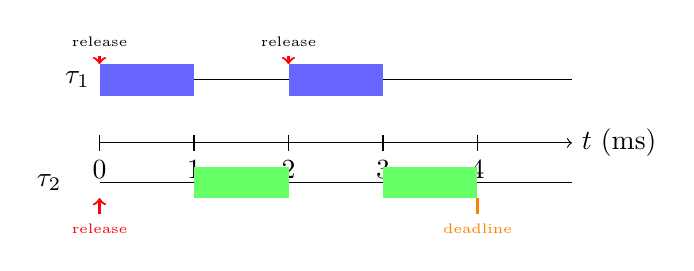
\begin{tikzpicture}[xscale=1.2]
    % Time axis
    \draw[->] (0,0) -- (5,0) node[right] {$t$ (ms)};
    \foreach \x in {0,1,2,3,4} {
        \draw (\x,0.1) -- (\x,-0.1) node[below] {\x};
    }

    % Task 1 timeline
    \draw (0,0.8) -- (5,0.8);
    \node[left] at (0,0.8) {$\tau_1$};
    \fill[blue!60] (0,0.6) rectangle (1,1.0);
    \fill[blue!60] (2,0.6) rectangle (3,1.0);
    \draw[red,thick,->] (0,1.1) -- (0,1.0);
    \draw[red,thick,->] (2,1.1) -- (2,1.0);
    \node[above,font=\tiny] at (0,1.1) {release};
    \node[above,font=\tiny] at (2,1.1) {release};

    % Task 2 timeline
    \draw (0,-0.5) -- (5,-0.5);
    \node[left] at (-0.3,-0.5) {$\tau_2$};
    \fill[green!60] (1,-0.7) rectangle (2,-0.3);
    \fill[green!60] (3,-0.7) rectangle (4,-0.3);
    \draw[red,thick,->] (0,-0.9) -- (0,-0.7);
    \node[below,font=\tiny,red] at (0,-0.9) {release};
    \draw[orange,thick] (4,-0.9) -- (4,-0.7);
    \node[below,font=\tiny,orange] at (4,-0.9) {deadline};
\end{tikzpicture}
\end{center}

\textbf{Timeline analysis} (critical instant at $t = 0$):
\begin{enumerate}
    \item $t = 0$: Both tasks release. $\tau_1$ has higher priority (shorter period), runs first.
    \item $t = 1$: $\tau_1$ completes. $\tau_2$ starts executing.
    \item $t = 2$: $\tau_1$ releases again, preempts $\tau_2$. ($\tau_2$ has executed 1 ms so far.)
    \item $t = 3$: $\tau_1$ completes. $\tau_2$ resumes.
    \item $t = 4$: $\tau_2$ completes (total execution: 1 + 1 = 2 ms). Deadline met exactly!
\end{enumerate}

Response time of $\tau_2$: $R_2 = 4$ ms $= D_2$. The task meets its deadline with zero slack.

\textbf{Why does this work?} The periods are harmonic ($T_2 = 2 T_1$), so $\tau_1$'s interference fits perfectly into $\tau_2$'s period. There are no wasted gaps---every millisecond is used productively.

This demonstrates that the Liu-Layland bound is \textbf{sufficient but not necessary}: failing the test does not mean the system is unschedulable.
\end{example}

\subsection{Response-Time Analysis}

Response-Time Analysis~\cite{audsley1993applying} computes the worst-case response time for each task and compares it to the deadline.

\begin{definition}[Response Time]
The \textbf{response time} $R_i$ of a task is the time from release to completion in the worst case.
\end{definition}

A task is schedulable if and only if:
\[
R_i \leq D_i
\]

\subsubsection{Computing Response Time}

The response time consists of:
\begin{itemize}
    \item The task's own execution time $C_i$
    \item Interference from higher-priority tasks $I_i$
\end{itemize}

\[
R_i = C_i + I_i
\]

During $R_i$, each higher-priority task $j$ executes $\lceil R_i / T_j \rceil$ times, each taking up to $C_j$ time:

\[
I_i = \sum_{j \in hp(i)} \left\lceil \frac{R_i}{T_j} \right\rceil C_j
\]

where $hp(i)$ is the set of tasks with higher priority than task $i$.

Combining:
\[
R_i = C_i + \sum_{j \in hp(i)} \left\lceil \frac{R_i}{T_j} \right\rceil C_j
\]

\textbf{Problem}: $R_i$ appears on both sides! This is a fixed-point equation.

\subsubsection{Iterative Solution}

Solve by iteration:

\[
w_i^{(k+1)} = C_i + \sum_{j \in hp(i)} \left\lceil \frac{w_i^{(k)}}{T_j} \right\rceil C_j
\]

Start with $w_i^{(0)} = C_i$ and iterate until convergence ($w_i^{(k+1)} = w_i^{(k)}$) or until $w_i^{(k)} > D_i$ (deadline miss).

\begin{example}[Response-Time Analysis]
Consider three tasks:

\begin{center}
\begin{tabular}{cccc}
\toprule
Task & $C_i$ (ms) & $T_i$ (ms) & Priority \\
\midrule
$\tau_1$ & 3 & 7 & High \\
$\tau_2$ & 3 & 12 & Medium \\
$\tau_3$ & 5 & 20 & Low \\
\bottomrule
\end{tabular}
\end{center}

\textbf{Task 1} (highest priority, no interference):
\[
R_1 = C_1 = 3 \text{ ms} \leq D_1 = 7 \text{ ms} \quad \checkmark
\]

\textbf{Task 2} (interference from Task 1):
\begin{align*}
w_2^{(0)} &= 3 \\
w_2^{(1)} &= 3 + \lceil 3/7 \rceil \cdot 3 = 3 + 1 \cdot 3 = 6 \\
w_2^{(2)} &= 3 + \lceil 6/7 \rceil \cdot 3 = 3 + 1 \cdot 3 = 6 \quad \text{(converged)}
\end{align*}
$R_2 = 6$ ms $\leq D_2 = 12$ ms $\checkmark$

\textbf{Task 3} (interference from Tasks 1 and 2):
\begin{align*}
w_3^{(0)} &= 5 \\
w_3^{(1)} &= 5 + \lceil 5/7 \rceil \cdot 3 + \lceil 5/12 \rceil \cdot 3 = 5 + 3 + 3 = 11 \\
w_3^{(2)} &= 5 + \lceil 11/7 \rceil \cdot 3 + \lceil 11/12 \rceil \cdot 3 = 5 + 6 + 3 = 14 \\
w_3^{(3)} &= 5 + \lceil 14/7 \rceil \cdot 3 + \lceil 14/12 \rceil \cdot 3 = 5 + 6 + 6 = 17 \\
w_3^{(4)} &= 5 + \lceil 17/7 \rceil \cdot 3 + \lceil 17/12 \rceil \cdot 3 = 5 + 9 + 6 = 20 \\
w_3^{(5)} &= 5 + \lceil 20/7 \rceil \cdot 3 + \lceil 20/12 \rceil \cdot 3 = 5 + 9 + 6 = 20 \quad \text{(converged)}
\end{align*}
$R_3 = 20$ ms $\leq D_3 = 20$ ms $\checkmark$ (just meets deadline!)
\end{example}

\begin{keyidea}[title=Response-Time Analysis is Exact]
Unlike the utilization bound, Response-Time Analysis is \textbf{sufficient and necessary}:
\begin{itemize}
    \item If the test passes, the system will meet all deadlines
    \item If the test fails, a deadline will be missed at runtime
\end{itemize}
This makes it the preferred method for verifying flight controller schedulability.
\end{keyidea}

\subsubsection{Proof Sketch: Why Response-Time Analysis Works}

We establish four key results that justify the response-time equation and its exactness.

\textbf{Result 1: Critical Instant Theorem.}
The worst-case response time for task $\tau_i$ occurs when it is released simultaneously with all higher-priority tasks (the \emph{critical instant}).

\emph{Intuition}: Any other release pattern means some higher-priority tasks release later, reducing interference during $\tau_i$'s response window.

\emph{Sketch}: Consider $\tau_i$ released at time $t_0$. If a higher-priority task $\tau_j$ releases at $t_0 - \delta$ (before $\tau_i$), it might complete before $\tau_i$ needs to run. If $\tau_j$ releases at $t_0 + \delta$ (after $\tau_i$), interference is delayed. Both cases reduce or maintain---but never increase---total interference compared to simultaneous release.

\textbf{Result 2: Interference Calculation.}
During response time $R_i$, each higher-priority task $\tau_j$ causes interference:
\[
I_{i,j} = \left\lceil \frac{R_i}{T_j} \right\rceil C_j
\]

\emph{Intuition}: In the interval $[0, R_i]$, task $\tau_j$ releases $\lceil R_i/T_j \rceil$ times, each execution consuming $C_j$ time units.

\emph{Sketch}: At the critical instant, $\tau_j$ first releases at $t = 0$, with subsequent releases at $T_j, 2T_j, 3T_j, \ldots$ The number of releases in $[0, R_i]$ is $\lfloor R_i/T_j \rfloor + 1 = \lceil R_i/T_j \rceil$, where the $+1$ accounts for the release at $t = 0$.

\begin{center}
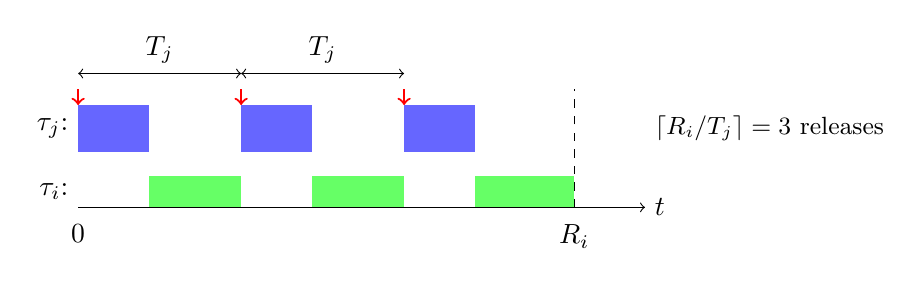
\begin{tikzpicture}[xscale=0.9]
    % Time axis
    \draw[->] (0,0) -- (8,0) node[right] {$t$};
    \node[below] at (0,-0.1) {$0$};
    \node[below] at (7,-0.1) {$R_i$};
    \draw[dashed] (7,0) -- (7,1.5);

    % Task j releases and executions
    \node[left] at (0,1) {$\tau_j$:};
    \fill[blue!60] (0,0.7) rectangle (1,1.3);
    \fill[blue!60] (2.3,0.7) rectangle (3.3,1.3);
    \fill[blue!60] (4.6,0.7) rectangle (5.6,1.3);

    % Release arrows
    \draw[->,red,thick] (0,1.5) -- (0,1.3);
    \draw[->,red,thick] (2.3,1.5) -- (2.3,1.3);
    \draw[->,red,thick] (4.6,1.5) -- (4.6,1.3);

    % Period markers
    \draw[<->] (0,1.7) -- (2.3,1.7) node[midway,above] {$T_j$};
    \draw[<->] (2.3,1.7) -- (4.6,1.7) node[midway,above] {$T_j$};

    % Task i (fragmented)
    \node[left] at (0,0.2) {$\tau_i$:};
    \fill[green!60] (1,0) rectangle (2.3,0.4);
    \fill[green!60] (3.3,0) rectangle (4.6,0.4);
    \fill[green!60] (5.6,0) rectangle (7,0.4);

    % Annotation
    \node[right,font=\small] at (8,1) {$\lceil R_i/T_j \rceil = 3$ releases};
\end{tikzpicture}
\end{center}

\textbf{Result 3: Fixed-Point Convergence.}
The iteration $w_i^{(k+1)} = C_i + \sum_{j \in hp(i)} \lceil w_i^{(k)}/T_j \rceil C_j$ converges to the response time.

\emph{Sketch}:
\begin{itemize}
    \item The right-hand side $f(w) = C_i + \sum_j \lceil w/T_j \rceil C_j$ is monotonically non-decreasing in $w$
    \item $f(w)$ is a step function, increasing only at multiples of period $T_j$
    \item Starting from $w^{(0)} = C_i$: since $w^{(1)} = f(w^{(0)}) \geq w^{(0)}$, the sequence is non-decreasing
    \item If $w^{(k+1)} = w^{(k)}$, we have found the fixed point $R_i$
    \item If $w^{(k)} > D_i$, the task is unschedulable and iteration terminates
    \item Termination is guaranteed: there are only finitely many step increases in $[C_i, D_i]$
\end{itemize}

\textbf{Result 4: Sufficiency and Necessity.}
Response-time analysis is both sufficient \emph{and} necessary, unlike the Liu-Layland bound.

\emph{Why sufficient}: If $R_i \leq D_i$, the task completes by its deadline even in the worst case (the critical instant).

\emph{Why necessary}: If $R_i > D_i$, then at the critical instant---which can actually occur (e.g., at system startup when all tasks release simultaneously)---the task misses its deadline. This is a real failure scenario, not a conservative bound.

\emph{Contrast with Liu-Layland}: The Liu-Layland bound assumes worst-case \emph{period relationships} (the maximally non-harmonic case) that may not exist in the actual task set. Response-time analysis uses the \emph{actual} task parameters, making it exact.

\begin{notebox}[title=Practical Implication]
For flight controller certification, response-time analysis provides the definitive answer:
\begin{itemize}
    \item \textbf{Pass}: The system \emph{will} meet all deadlines under all conditions
    \item \textbf{Fail}: There \emph{exists} a scenario (the critical instant) where a deadline is missed
\end{itemize}
This exactness is why response-time analysis is preferred over utilization bounds in safety-critical systems, despite requiring more computation.
\end{notebox}

\subsection{Accounting for Blocking}

When tasks share resources (mutexes), low-priority tasks can block high-priority tasks. This adds a \textbf{blocking term} $B_i$ to the response time:

\[
R_i = C_i + B_i + \sum_{j \in hp(i)} \left\lceil \frac{R_i}{T_j} \right\rceil C_j
\]

where $B_i$ is the maximum time task $i$ can be blocked by lower-priority tasks holding mutexes.

With priority inheritance, $B_i$ is bounded by the longest critical section of any lower-priority task that uses a mutex also used by task $i$ or any higher-priority task.

\section{Cyclic Executives}

Before RTOS became common, many real-time systems used \textbf{cyclic executives}:

\begin{definition}[Cyclic Executive]
A \textbf{cyclic executive} is a scheduling approach where the programmer manually constructs a fixed schedule that repeats periodically. Tasks are implemented as procedures called at predetermined times.
\end{definition}

\begin{example}[Cyclic Executive Schedule]
\begin{center}
\begin{tabular}{ccc}
\toprule
Task & Period (ms) & WCET (ms) \\
\midrule
A & 25 & 10 \\
B & 25 & 8 \\
C & 50 & 5 \\
D & 50 & 4 \\
E & 100 & 2 \\
\bottomrule
\end{tabular}
\end{center}

Minor cycle: 25 ms, Major cycle: 100 ms

\begin{center}
\begin{tabular}{c|cccc}
\toprule
Minor cycle & 1 & 2 & 3 & 4 \\
\midrule
Tasks & A, B, C, E & A, B, D & A, B, C & A, B, D \\
\bottomrule
\end{tabular}
\end{center}
\end{example}

\textbf{Advantages}:
\begin{itemize}
    \item Fully deterministic---exact same execution every major cycle
    \item Very low overhead (no scheduler, no context switches within minor cycle)
    \item Easy to verify timing
\end{itemize}

\textbf{Disadvantages}:
\begin{itemize}
    \item \textbf{Cannot handle sporadic events} (external inputs at unpredictable times)
    \item \textbf{Difficult to construct} (finding a valid schedule is NP-hard)
    \item \textbf{Difficult to modify} (adding a task may require redesigning the entire schedule)
    \item \textbf{Large tasks must be split} into pieces that fit in minor cycles
\end{itemize}

\begin{notebox}[title=When to Use Cyclic Executives]
Cyclic executives are still used in highly safety-critical systems (e.g., aircraft fly-by-wire) where determinism is paramount and the task set is fixed. For quadrotor flight controllers with varying requirements and rapid development cycles, RTOS-based scheduling is more practical.
\end{notebox}


\chapter{Latency and Jitter in Control Systems}

\section{Introduction: Why Timing Affects Control}

Control theory typically assumes:
\begin{itemize}
    \item Instantaneous sampling (sensor values captured at exact times)
    \item Instantaneous computation (control law evaluates in zero time)
    \item Instantaneous actuation (outputs applied immediately)
\end{itemize}

Reality is different:
\begin{itemize}
    \item Sampling takes time (ADC conversion, communication)
    \item Computation takes time (running control algorithm)
    \item Actuation takes time (PWM update, motor response)
\end{itemize}

These delays, and variations in these delays, affect control performance.

\section{Timing Definitions}

Consider a periodic control task with period $T$. Job $k$ is released at time $r_k = kT$.

\begin{definition}[Timing Parameters]
For each job $k$ of a control task:
\begin{itemize}
    \item $r_k$: \textbf{Release time} (when task becomes ready)
    \item $s_k$: \textbf{Start time} (when task begins executing)
    \item $f_k$: \textbf{Finish time} (when task completes)
    \item $R_k = f_k - r_k$: \textbf{Response time}
\end{itemize}
\end{definition}

\begin{definition}[Latency]
\begin{itemize}
    \item \textbf{Sampling latency} $L^s_k = s_k - r_k$: Delay from release to when input is sampled
    \item \textbf{Input-output latency} $L^{io}_k = f_k - r_k$: Delay from release to when output is applied
\end{itemize}
\end{definition}

\begin{definition}[Jitter]
\begin{itemize}
    \item \textbf{Sampling jitter} $J^s = \max_k L^s_k - \min_k L^s_k$: Variation in sampling times
    \item \textbf{Input-output jitter} $J^{io} = \max_k L^{io}_k - \min_k L^{io}_k$: Variation in output times
\end{itemize}
\end{definition}

\textbf{Intuition}:
\begin{itemize}
    \item \textbf{Latency} is like a constant time delay---it shifts the control response but doesn't destabilize (within limits).
    \item \textbf{Jitter} is like a randomly varying time delay---it makes the system non-deterministic and can cause oscillations or instability.
\end{itemize}

\section{Effect of Latency on Control}

A control system with sampling period $T$ and computational delay $\tau$ behaves like a continuous system with time delay $\tau + T/2$ (on average).

\textbf{Effect on stability}: Time delay adds negative phase to the loop gain:
\[
\Delta\phi = -\omega_c \tau_{total}
\]
where $\omega_c$ is the crossover frequency.

\begin{example}[Phase Margin Degradation]
Quadrotor attitude loop: $\omega_c = 20$ rad/s, designed phase margin 45°

If computational delay $\tau = 2$ ms:
\[
\Delta\phi = -20 \times 0.002 = -0.04 \text{ rad} = -2.3°
\]

Remaining phase margin: $45° - 2.3° = 42.7°$---still adequate.

If delay increases to $\tau = 10$ ms:
\[
\Delta\phi = -20 \times 0.010 = -0.2 \text{ rad} = -11.5°
\]

Remaining phase margin: $45° - 11.5° = 33.5°$---getting marginal.
\end{example}

\begin{keyidea}[title=Latency Design Rule]
For a control loop with crossover frequency $\omega_c$, total latency should satisfy:
\[
\tau_{total} < \frac{\phi_{margin}}{2 \omega_c}
\]
where $\phi_{margin}$ is the design phase margin in radians.

For a 45° (0.79 rad) phase margin and $\omega_c = 20$ rad/s:
\[
\tau_{total} < \frac{0.79}{2 \times 20} = 20 \text{ ms}
\]
\end{keyidea}

\section{Effect of Jitter on Control}

Jitter is more problematic than constant latency because:

\begin{enumerate}
    \item \textbf{Non-uniform sampling}: The control law assumes uniform $T$, but actual intervals vary
    \item \textbf{Time-varying delay}: Cannot be compensated by fixed controller design
    \item \textbf{Can excite resonances}: Random timing can inject energy at problematic frequencies
\end{enumerate}

\begin{warningbox}[title=Jitter Sensitivity]
As a rule of thumb, jitter should be less than 1\% of the sampling period:
\[
J < 0.01 \times T
\]

For attitude control at 500 Hz ($T = 2$ ms):
\[
J < 20 \text{ }\mu\text{s}
\]

This is achievable with careful RTOS design but requires attention to:
\begin{itemize}
    \item Priority assignment (control task must have highest priority)
    \item Interrupt latency (ISR overhead)
    \item Critical section length (blocking time)
\end{itemize}
\end{warningbox}

\section{Reducing Latency with Subtask Scheduling}

A control algorithm typically has this structure:

\begin{lstlisting}[language=C]
void ControlTask(void) {
    while (1) {
        y = ReadSensor();        // Input
        u = ControlLaw(y, x);    // Calculate output
        WriteActuator(u);        // Output
        x = UpdateState(y, u);   // Update internal state
        WaitNextPeriod();
    }
}
\end{lstlisting}

\textbf{Observation}: The \texttt{UpdateState} doesn't affect the \emph{current} output---it only prepares for the \emph{next} sample. We can defer it!

\subsection{Subtask Decomposition}

Split the control task into two subtasks:

\begin{lstlisting}[language=C, caption=Subtask decomposition]
// High priority: Calculate and Output
void ControlOutputTask(void) {
    while (1) {
        WaitForSensor();         // Triggered by sensor
        y = ReadSensor();
        u = ControlLaw(y, x);    // Use state from previous cycle
        WriteActuator(u);
        SignalUpdateTask();      // Tell update task to run
    }
}

// Lower priority: Update State
void StateUpdateTask(void) {
    while (1) {
        WaitForSignal();         // Wait for output task
        x = UpdateState(y, u);   // Can be preempted
    }
}
\end{lstlisting}

\textbf{Benefits}:
\begin{itemize}
    \item \textbf{Shorter critical path}: Input $\to$ Output latency is minimized
    \item \textbf{State update runs in ``slack time''}: Between output and next sample
    \item \textbf{Other tasks can preempt update}: Doesn't affect I/O latency
\end{itemize}

\subsection{Deadline Assignment for Subtasks}

For a control task with period $T$ and WCET split as:
\begin{itemize}
    \item $C_{CO}$: Calculate Output WCET
    \item $C_{US}$: Update State WCET
\end{itemize}

Assign deadlines:
\begin{itemize}
    \item $D_{CO}$: As short as possible (minimize I/O latency)
    \item $D_{US} = T$: Full period (less critical)
\end{itemize}

\begin{example}[Inverted Pendulum Case Study]
Three inverted pendulums controlled by one CPU:
\begin{center}
\begin{tabular}{lccc}
\toprule
Pendulum & Period & Standard RMS & Subtask Scheduling \\
\midrule
1 (fastest) & 10 ms & 1.5 ms latency & 1.5 ms latency \\
2 & 14.5 ms & 4.5 ms latency & 3.0 ms latency \\
3 (slowest) & 17.5 ms & \textbf{Unstable!} & 4.5 ms latency \\
\bottomrule
\end{tabular}
\end{center}

With standard RMS, the lowest-priority pendulum becomes unstable due to excessive latency. With subtask scheduling, all three are stable because the I/O path is prioritized.
\end{example}

\section{Measuring Timing in Practice}

\subsection{GPIO-Based Measurement}

The simplest way to measure task timing is with GPIO pins and an oscilloscope:

\begin{lstlisting}[language=C, caption=GPIO timing measurement]
#define TIMING_PIN  GPIO_PIN_0

void ControlTask(void *pvParameters) {
    for (;;) {
        GPIO_SetHigh(TIMING_PIN);   // Rising edge: start

        // Control computation
        ReadSensors();
        ComputeControl();
        WriteActuators();

        GPIO_SetLow(TIMING_PIN);    // Falling edge: end

        vTaskDelayUntil(&xLastWakeTime, pdMS_TO_TICKS(2));
    }
}
\end{lstlisting}

\textbf{What to measure}:
\begin{itemize}
    \item \textbf{Pulse width}: Execution time
    \item \textbf{Pulse period}: Actual task period (should be constant)
    \item \textbf{Period variation}: Jitter
\end{itemize}

\subsection{Software Timestamps}

\begin{lstlisting}[language=C, caption=Software jitter measurement]
void ControlTask(void *pvParameters) {
    TickType_t xLastWakeTime = xTaskGetTickCount();
    uint32_t lastTimestamp = 0;

    for (;;) {
        uint32_t now = GetHighResTimer();  // Microsecond timer
        uint32_t period = now - lastTimestamp;
        lastTimestamp = now;

        // Check for jitter
        int32_t jitter = period - EXPECTED_PERIOD_US;
        if (abs(jitter) > MAX_ALLOWED_JITTER_US) {
            LogJitterEvent(jitter);
        }

        // Control computation...

        vTaskDelayUntil(&xLastWakeTime, pdMS_TO_TICKS(2));
    }
}
\end{lstlisting}

\subsection{Trace Tools}

For detailed timing analysis:

\begin{itemize}
    \item \textbf{Segger SystemView}: Free tool for FreeRTOS, shows task execution timeline
    \item \textbf{Tracealyzer}: Commercial tool with advanced analysis features
    \item \textbf{Logic analyzer}: Hardware capture of GPIO timing signals
\end{itemize}


\chapter{Worst-Case Execution Time Estimation}

\section{Introduction: Why WCET Matters}

Schedulability analysis requires knowing the \textbf{worst-case execution time (WCET)} of each task. If we underestimate WCET, the system may miss deadlines even though analysis said it wouldn't.

\textbf{The challenge}: Execution time varies depending on:
\begin{itemize}
    \item Input data (different code paths)
    \item Cache state (hits vs. misses)
    \item Pipeline state (branch prediction)
    \item Interrupt timing
\end{itemize}

Finding the true worst case is difficult---and for complex processors, often impossible to determine exactly.

\section{Why WCET Estimation Is Hard}

\subsection{Program Path Variability}

\begin{lstlisting}[language=C, caption=Code with variable execution time]
void ProcessSensorData(SensorData_t *data) {
    // Path 1: Normal processing
    if (data->status == VALID) {
        ApplyCalibration(data);      // Fast path
    }
    // Path 2: Error handling
    else {
        LogError(data);              // Slower path
        AttemptRecovery(data);       // Even slower
    }

    // Loop with data-dependent iteration count
    for (int i = 0; i < data->numSamples; i++) {
        ProcessSample(&data->samples[i]);
    }
}
\end{lstlisting}

The execution time depends on:
\begin{itemize}
    \item Whether the data is valid
    \item How many samples need processing
    \item Whether recovery succeeds
\end{itemize}

\subsection{Hardware Effects}

\textbf{Cache}: First access to memory is slow (cache miss); subsequent accesses to same region are fast (cache hit). The cache state depends on what ran before.

\textbf{Pipeline}: Modern processors execute multiple instructions simultaneously. Branch mispredictions cause pipeline flushes, adding cycles.

\textbf{Memory wait states}: External memory (Flash, SDRAM) is slower than internal SRAM. Access patterns affect timing.

\begin{notebox}[title=ARM Cortex-M4 Timing Characteristics]
The STM32F4 (Crazyflie main processor) has:
\begin{itemize}
    \item 3-stage pipeline with branch prediction
    \item Instruction and data caches
    \item Flash memory with wait states (up to 7 cycles at 168 MHz)
    \item Single-cycle multiply, multi-cycle divide
\end{itemize}
These features make WCET estimation non-trivial even for a ``simple'' embedded processor.
\end{notebox}

\section{WCET Estimation Methods}

\subsection{Measurement-Based Estimation}

Run the code many times with different inputs and measure execution time.

\begin{lstlisting}[language=C, caption=Measurement-based WCET estimation]
#define NUM_TESTS 10000

uint32_t MeasureWCET(void (*task)(void*), void *params) {
    uint32_t maxTime = 0;

    for (int i = 0; i < NUM_TESTS; i++) {
        // Vary inputs to cover different paths
        GenerateTestInput(params, i);

        uint32_t start = GetCycleCount();
        task(params);
        uint32_t elapsed = GetCycleCount() - start;

        if (elapsed > maxTime) {
            maxTime = elapsed;
        }
    }

    return maxTime;
}
\end{lstlisting}

\textbf{Advantages}:
\begin{itemize}
    \item Simple to implement
    \item Measures real hardware behavior
    \item Catches hardware effects automatically
\end{itemize}

\textbf{Disadvantages}:
\begin{itemize}
    \item May not find the true worst case (input coverage problem)
    \item Results depend on test inputs
    \item Time-consuming for thorough coverage
\end{itemize}

\begin{keyidea}[title=Adding Safety Margin]
Since measurement may not find the true worst case, add a safety margin:
\[
WCET_{design} = \alpha \times WCET_{measured}
\]
Typical values: $\alpha = 1.2$ to $1.5$ (20--50\% margin)

The margin accounts for:
\begin{itemize}
    \item Untested input combinations
    \item Cache state variations
    \item Interrupt interference
\end{itemize}
\end{keyidea}

\subsection{Static Analysis}

Analyze the code without running it to compute a safe upper bound.

\textbf{Steps}:
\begin{enumerate}
    \item Build control flow graph (all possible paths)
    \item Determine loop bounds (maximum iterations)
    \item Model processor timing (cycles per instruction)
    \item Find longest path
\end{enumerate}

\textbf{Tools}:
\begin{itemize}
    \item aiT (AbsInt): Commercial, widely used in aerospace
    \item OTAWA: Open-source, academic
    \item Bound-T: Originally from Tidorum, now discontinued
\end{itemize}

\textbf{Advantages}:
\begin{itemize}
    \item Produces safe upper bound (no underestimation)
    \item Covers all paths automatically
    \item Can handle complex code
\end{itemize}

\textbf{Disadvantages}:
\begin{itemize}
    \item Often overly pessimistic (over-estimates WCET)
    \item Requires processor timing model
    \item May need manual annotations for loop bounds
    \item Expensive tools
\end{itemize}

\subsection{Hybrid Approach}

Combine measurement and analysis:

\begin{enumerate}
    \item Use static analysis to identify worst-case paths
    \item Use measurement to get accurate timing for those paths
    \item Add margin for hardware variability
\end{enumerate}

\section{Practical WCET Estimation for Quadrotors}

\subsection{Strategy for Flight Controller Code}

\begin{enumerate}
    \item \textbf{Profile each task} with representative inputs:
    \begin{lstlisting}[language=C]
    uint32_t start = DWT->CYCCNT;
    RunAttitudeControl();
    uint32_t cycles = DWT->CYCCNT - start;
    float timeMs = cycles / (SystemCoreClock / 1000.0f);
    \end{lstlisting}

    \item \textbf{Test edge cases}: Sensor saturation, maximum rates, error conditions

    \item \textbf{Add 30--50\% margin} for safety

    \item \textbf{Monitor at runtime} to detect if estimates are exceeded:
    \begin{lstlisting}[language=C]
    if (actualTime > WCET_ESTIMATE) {
        LogOverrun(taskId, actualTime);
    }
    \end{lstlisting}
\end{enumerate}

\subsection{Code Design for Predictable Timing}

\begin{keyidea}[title=Writing Timing-Predictable Code]
\begin{enumerate}
    \item \textbf{Avoid data-dependent loops}: Use fixed iteration counts where possible
    \item \textbf{Minimize branching}: Especially in inner loops
    \item \textbf{Use lookup tables}: Faster and more predictable than computation
    \item \textbf{Avoid dynamic memory}: \texttt{malloc}/\texttt{free} have variable timing
    \item \textbf{Bound iterations}: Add maximum iteration limits to all loops
    \item \textbf{Avoid recursion}: Stack depth is hard to bound
\end{enumerate}
\end{keyidea}

\begin{lstlisting}[language=C, caption=Timing-predictable code patterns]
// BAD: Data-dependent loop bound
for (int i = 0; i < sensor.numReadings; i++) { ... }

// GOOD: Fixed bound with early exit
for (int i = 0; i < MAX_READINGS; i++) {
    if (i >= sensor.numReadings) break;
    ...
}

// BAD: Unbounded iteration
while (!converged) {
    iterate();
}

// GOOD: Bounded iteration
for (int iter = 0; iter < MAX_ITERATIONS && !converged; iter++) {
    iterate();
}
\end{lstlisting}


\chapter{Fault Detection and Recovery}

\section{Introduction: Why Fault Handling Matters}

In a safety-critical system like a flight controller, things go wrong:
\begin{itemize}
    \item Tasks may take longer than expected (overrun)
    \item Sensors may fail or produce invalid data
    \item Communication may be lost
    \item Software bugs may cause unexpected behavior
\end{itemize}

A well-designed system detects these faults and recovers gracefully rather than crashing.

\section{Watchdog Timers}

\subsection{Hardware Watchdog}

A \textbf{hardware watchdog} is a countdown timer that resets the processor if not periodically ``fed'' by software.

\begin{lstlisting}[language=C, caption=Hardware watchdog usage]
// Initialize watchdog with 100ms timeout
void InitWatchdog(void) {
    IWDG->KR = 0x5555;  // Enable register access
    IWDG->PR = 4;       // Prescaler
    IWDG->RLR = 1000;   // Reload value (~100ms)
    IWDG->KR = 0xCCCC;  // Start watchdog
}

// Feed watchdog (call from main loop or dedicated task)
void FeedWatchdog(void) {
    IWDG->KR = 0xAAAA;  // Reload counter
}

// If FeedWatchdog() is not called within 100ms, processor resets!
\end{lstlisting}

\textbf{Design pattern}: Feed the watchdog only when the system is healthy:

\begin{lstlisting}[language=C, caption=Watchdog feeding strategy]
void WatchdogTask(void *pvParameters) {
    for (;;) {
        // Check system health
        bool healthy = true;
        healthy &= AttitudeControlRunning();
        healthy &= SensorFusionRunning();
        healthy &= MotorOutputValid();

        if (healthy) {
            FeedWatchdog();
        }
        // If unhealthy, don't feed -> system resets

        vTaskDelay(pdMS_TO_TICKS(20));
    }
}
\end{lstlisting}

\subsection{Software Watchdogs}

\textbf{Software watchdogs} monitor individual tasks without resetting the entire system:

\begin{lstlisting}[language=C, caption=Software watchdog for tasks]
typedef struct {
    TickType_t lastActivity;
    TickType_t timeout;
    bool healthy;
} TaskWatchdog_t;

TaskWatchdog_t taskWatchdogs[NUM_TASKS];

// Called by each task when it runs
void TaskCheckin(int taskId) {
    taskWatchdogs[taskId].lastActivity = xTaskGetTickCount();
    taskWatchdogs[taskId].healthy = true;
}

// Monitoring task
void WatchdogMonitorTask(void *pvParameters) {
    for (;;) {
        TickType_t now = xTaskGetTickCount();

        for (int i = 0; i < NUM_TASKS; i++) {
            TickType_t elapsed = now - taskWatchdogs[i].lastActivity;
            if (elapsed > taskWatchdogs[i].timeout) {
                taskWatchdogs[i].healthy = false;
                HandleTaskTimeout(i);
            }
        }

        vTaskDelay(pdMS_TO_TICKS(10));
    }
}
\end{lstlisting}

\section{Deadline Miss Detection}

\begin{lstlisting}[language=C, caption=Deadline miss detection]
void ControlTask(void *pvParameters) {
    TickType_t xLastWakeTime = xTaskGetTickCount();
    const TickType_t xPeriod = pdMS_TO_TICKS(2);

    for (;;) {
        TickType_t startTime = xTaskGetTickCount();

        // Control computation
        ReadSensors();
        ComputeControl();
        WriteActuators();

        // Check deadline
        TickType_t endTime = xTaskGetTickCount();
        TickType_t expectedEnd = xLastWakeTime + xPeriod;

        if (endTime > expectedEnd) {
            // Deadline missed!
            g_deadlineMissCount++;
            LogDeadlineMiss(TASK_CONTROL, endTime - expectedEnd);

            if (g_consecutiveMisses++ > MAX_CONSECUTIVE_MISSES) {
                TriggerFailsafe();
            }
        } else {
            g_consecutiveMisses = 0;
        }

        vTaskDelayUntil(&xLastWakeTime, xPeriod);
    }
}
\end{lstlisting}

\section{Failsafe Behavior}

\subsection{Failsafe Hierarchy}

\begin{center}
\begin{tabular}{lll}
\toprule
\textbf{Fault} & \textbf{Detection} & \textbf{Response} \\
\midrule
Single deadline miss & Runtime monitoring & Log, continue \\
Multiple deadline misses & Consecutive count & Reduce performance \\
Sensor failure & Validation checks & Use backup/estimate \\
Communication loss & Timeout & Return to home \\
Critical failure & Watchdog & Controlled descent \\
Catastrophic failure & Hardware watchdog & System reset \\
\bottomrule
\end{tabular}
\end{center}

\subsection{Graceful Degradation}

\begin{lstlisting}[language=C, caption=Graceful degradation example]
typedef enum {
    MODE_FULL_AUTONOMOUS,   // All systems nominal
    MODE_REDUCED_AUTONOMY,  // Some systems degraded
    MODE_MANUAL_ONLY,       // Autopilot disabled
    MODE_FAILSAFE_DESCENT,  // Controlled descent
    MODE_EMERGENCY_STOP     // Motors off
} FlightMode_t;

void HandleFault(FaultType_t fault) {
    switch (fault) {
        case FAULT_GPS_LOST:
            if (currentMode == MODE_FULL_AUTONOMOUS) {
                currentMode = MODE_REDUCED_AUTONOMY;
                DisablePositionControl();
                // Can still fly manually with attitude control
            }
            break;

        case FAULT_IMU_FAILURE:
            // Critical - cannot maintain attitude
            currentMode = MODE_EMERGENCY_STOP;
            DisarmMotors();
            break;

        case FAULT_RADIO_LOST:
            currentMode = MODE_FAILSAFE_DESCENT;
            InitiateControlledDescent();
            break;
    }
}
\end{lstlisting}

\section{Practical Recommendations}

\begin{keyidea}[title=Fault Handling Best Practices]
\begin{enumerate}
    \item \textbf{Always use a hardware watchdog}: Last line of defense against software lockup
    \item \textbf{Monitor task health}: Each critical task should check in regularly
    \item \textbf{Log faults}: Record timing anomalies for post-flight analysis
    \item \textbf{Define failsafe hierarchy}: Know what happens for each type of fault
    \item \textbf{Test failure modes}: Deliberately inject faults during development
    \item \textbf{Prefer degradation over shutdown}: Keep flying if at all possible
\end{enumerate}
\end{keyidea}


\chapter{Case Study: Complete Quadrotor Scheduler Design}

\section{System Requirements}

Design a flight controller scheduler with the following requirements:

\begin{center}
\begin{tabular}{lcc}
\toprule
\textbf{Function} & \textbf{Rate} & \textbf{Deadline} \\
\midrule
IMU sampling & 1000 Hz & Hard \\
Attitude control & 500 Hz & Hard \\
Sensor fusion & 500 Hz & Hard \\
Position control & 50 Hz & Firm \\
State estimation (EKF) & 50 Hz & Firm \\
Radio communication & 100 Hz & Soft \\
Telemetry logging & 10 Hz & Soft \\
Battery monitoring & 1 Hz & Soft \\
\bottomrule
\end{tabular}
\end{center}

\section{Task Design}

\subsection{Step 1: Measure WCET}

Profile each function on target hardware:

\begin{center}
\begin{tabular}{lcc}
\toprule
\textbf{Task} & \textbf{Measured Max} & \textbf{WCET (with 30\% margin)} \\
\midrule
IMU sampling & 50 $\mu$s & 65 $\mu$s \\
Attitude control & 180 $\mu$s & 235 $\mu$s \\
Sensor fusion & 150 $\mu$s & 195 $\mu$s \\
Position control & 400 $\mu$s & 520 $\mu$s \\
State estimation & 800 $\mu$s & 1040 $\mu$s \\
Radio communication & 500 $\mu$s & 650 $\mu$s \\
Telemetry logging & 2000 $\mu$s & 2600 $\mu$s \\
Battery monitoring & 100 $\mu$s & 130 $\mu$s \\
\bottomrule
\end{tabular}
\end{center}

\subsection{Step 2: Assign Priorities (RMS)}

\begin{center}
\begin{tabular}{lccc}
\toprule
\textbf{Task} & \textbf{Period} & \textbf{RMS Priority} & \textbf{FreeRTOS Priority} \\
\midrule
IMU sampling & 1 ms & 1 (highest) & 7 \\
Attitude control & 2 ms & 2 & 6 \\
Sensor fusion & 2 ms & 2 & 6 \\
Radio communication & 10 ms & 3 & 5 \\
Position control & 20 ms & 4 & 4 \\
State estimation & 20 ms & 4 & 4 \\
Telemetry logging & 100 ms & 5 & 3 \\
Battery monitoring & 1000 ms & 6 (lowest) & 2 \\
\bottomrule
\end{tabular}
\end{center}

\subsection{Step 3: Utilization Analysis}

\begin{center}
\begin{tabular}{lccc}
\toprule
\textbf{Task} & $C_i$ ($\mu$s) & $T_i$ ($\mu$s) & $U_i$ \\
\midrule
IMU sampling & 65 & 1000 & 6.5\% \\
Attitude control & 235 & 2000 & 11.75\% \\
Sensor fusion & 195 & 2000 & 9.75\% \\
Radio communication & 650 & 10000 & 6.5\% \\
Position control & 520 & 20000 & 2.6\% \\
State estimation & 1040 & 20000 & 5.2\% \\
Telemetry logging & 2600 & 100000 & 2.6\% \\
Battery monitoring & 130 & 1000000 & 0.013\% \\
\midrule
\textbf{Total} & & & \textbf{44.9\%} \\
\bottomrule
\end{tabular}
\end{center}

Liu-Layland bound for 8 tasks: $8(2^{1/8} - 1) = 72.4\%$

Since $44.9\% < 72.4\%$, the task set is \textbf{guaranteed schedulable}.

\subsection{Step 4: Response-Time Analysis}

For the lowest-priority task (Battery monitoring), we verify:

Since it has very long period (1000 ms) and all higher-priority tasks have low utilization, the response time is bounded by approximately:
\[
R_{battery} \approx C_{battery} + \sum_{higher} \frac{R_{battery}}{T_j} C_j
\]

Given the low total utilization, this converges well within the 1000 ms deadline.

\section{Synchronization Design}

\begin{lstlisting}[language=C, caption=Synchronization structure]
// Mutexes for shared state
SemaphoreHandle_t g_orientationMutex;  // Protects orientation estimate
SemaphoreHandle_t g_positionMutex;     // Protects position estimate
SemaphoreHandle_t g_setpointMutex;     // Protects control setpoints

// Queues for data flow
QueueHandle_t g_imuQueue;              // IMU -> Sensor Fusion
QueueHandle_t g_commandQueue;          // Radio -> Position Control
QueueHandle_t g_logQueue;              // All -> Logging

// Semaphores for event signaling
SemaphoreHandle_t g_imuDataReady;      // ISR -> IMU task
\end{lstlisting}

\section{Complete Implementation}

\begin{lstlisting}[language=C, caption=Complete flight controller initialization]
void FlightController_Init(void) {
    // Create synchronization primitives
    g_orientationMutex = xSemaphoreCreateMutex();
    g_positionMutex = xSemaphoreCreateMutex();
    g_setpointMutex = xSemaphoreCreateMutex();

    g_imuQueue = xQueueCreate(10, sizeof(ImuData_t));
    g_commandQueue = xQueueCreate(5, sizeof(Command_t));
    g_logQueue = xQueueCreate(50, sizeof(LogEntry_t));

    g_imuDataReady = xSemaphoreCreateBinary();

    // Create tasks (highest priority first)
    xTaskCreate(ImuTask,           "IMU",     256,  NULL, 7, NULL);
    xTaskCreate(AttitudeCtrlTask,  "AttCtrl", 512,  NULL, 6, NULL);
    xTaskCreate(SensorFusionTask,  "SensFus", 512,  NULL, 6, NULL);
    xTaskCreate(RadioTask,         "Radio",   256,  NULL, 5, NULL);
    xTaskCreate(PositionCtrlTask,  "PosCtrl", 512,  NULL, 4, NULL);
    xTaskCreate(StateEstTask,      "StateEst",1024, NULL, 4, NULL);
    xTaskCreate(LoggingTask,       "Log",     512,  NULL, 3, NULL);
    xTaskCreate(BatteryTask,       "Battery", 128,  NULL, 2, NULL);
    xTaskCreate(WatchdogTask,      "WDT",     128,  NULL, 1, NULL);

    // Initialize hardware watchdog
    InitHardwareWatchdog(200);  // 200ms timeout

    // Start scheduler
    vTaskStartScheduler();
}
\end{lstlisting}

%======================================================================
\chapter{Power Management for Flight Controllers}
%======================================================================

Power management is critical for battery-powered quadrotors. Effective power management extends flight time, prevents unexpected shutdowns, and ensures safe operation throughout the discharge cycle.

\section{Why Power Management Matters}

A quadrotor's flight time is fundamentally limited by battery capacity:

\[
t_{\text{flight}} = \frac{E_{\text{battery}}}{\overline{P}_{\text{total}}}
\]

where $E_{\text{battery}}$ is the battery energy (Wh) and $\overline{P}_{\text{total}}$ is the average power consumption. For a typical micro-quadrotor:

\begin{center}
\begin{tabular}{lcc}
\toprule
\textbf{Component} & \textbf{Power} & \textbf{Percentage} \\
\midrule
Motors (hover) & 3.5 W & 85--90\% \\
MCU & 0.2 W & 5\% \\
Sensors & 0.05 W & 1\% \\
Radio & 0.1 W & 2--3\% \\
Other (LED, etc.) & 0.05 W & 1--2\% \\
\bottomrule
\end{tabular}
\end{center}

While motors dominate power consumption, the flight controller's power management strategy affects safety and reliability.

\section{Battery Monitoring}

\subsection{Voltage Monitoring}

LiPo batteries have a characteristic discharge curve:

%----------------------------------------------------------------------
% FIGURE: LiPo Discharge Curve
%----------------------------------------------------------------------
% Description: Plot showing cell voltage vs. state of charge.
%
% X-axis: State of charge (0-100%)
% Y-axis: Cell voltage (3.0V - 4.2V)
%
% Show: Characteristic curve with:
%   - Full charge at 4.2V
%   - Nominal region around 3.7V
%   - Knee at ~3.5V where voltage drops rapidly
%   - Minimum safe voltage at 3.0V
%
% Mark danger zone below 3.0V.
% Dimensions: Column width, ~5cm height.
%----------------------------------------------------------------------

\begin{lstlisting}[language=C, caption=Battery voltage monitoring]
#define BATTERY_CELLS        1       // Single cell LiPo
#define CELL_FULL_VOLTAGE    4.2f    // Fully charged
#define CELL_NOMINAL_VOLTAGE 3.7f    // Nominal voltage
#define CELL_LOW_VOLTAGE     3.5f    // Low warning threshold
#define CELL_CRITICAL_VOLTAGE 3.3f   // Critical - land immediately
#define CELL_CUTOFF_VOLTAGE  3.0f    // Cutoff - damage risk

typedef struct {
    float voltage;           // Measured voltage [V]
    float current;           // Measured current [A] (if available)
    float capacity_mAh;      // Remaining capacity estimate
    uint8_t percentage;      // State of charge (0-100%)
    BatteryState_t state;    // Normal, Low, Critical, Cutoff
} BatteryStatus_t;

// ADC reading to voltage conversion
// Assumes voltage divider: Vbat -> R1 -> ADC -> R2 -> GND
float ADC_ToVoltage(uint16_t adc_reading)
{
    const float ADC_REF = 3.3f;       // ADC reference voltage
    const float ADC_MAX = 4095.0f;    // 12-bit ADC
    const float DIVIDER_RATIO = 2.0f; // R1 = R2, so ratio = 2

    float v_adc = (adc_reading / ADC_MAX) * ADC_REF;
    return v_adc * DIVIDER_RATIO;
}

// Apply low-pass filter to reduce noise
float BatteryVoltageFiltered(float new_reading)
{
    static float voltage_filtered = 4.2f;
    const float alpha = 0.1f;  // Filter coefficient

    voltage_filtered = alpha * new_reading + (1.0f - alpha) * voltage_filtered;
    return voltage_filtered;
}

// Estimate state of charge from voltage (open-circuit approximation)
// Note: This is approximate - accurate SOC requires current integration
uint8_t VoltageToSOC(float cell_voltage)
{
    // Piecewise linear approximation of LiPo discharge curve
    if (cell_voltage >= 4.2f) return 100;
    if (cell_voltage >= 4.0f) return 80 + (cell_voltage - 4.0f) * 100;
    if (cell_voltage >= 3.8f) return 40 + (cell_voltage - 3.8f) * 200;
    if (cell_voltage >= 3.6f) return 15 + (cell_voltage - 3.6f) * 125;
    if (cell_voltage >= 3.0f) return (cell_voltage - 3.0f) * 25;
    return 0;
}
\end{lstlisting}

\subsection{Current Monitoring and Coulomb Counting}

For accurate state-of-charge estimation, integrate current over time:

\begin{lstlisting}[language=C, caption=Coulomb counting for SOC estimation]
typedef struct {
    float capacity_mAh;      // Nominal battery capacity
    float consumed_mAh;      // Integrated consumption
    float current_filtered;  // Filtered current reading
    uint32_t last_update_ms; // Last integration time
} CoulombCounter_t;

void CoulombCounter_Init(CoulombCounter_t *cc, float capacity_mAh)
{
    cc->capacity_mAh = capacity_mAh;
    cc->consumed_mAh = 0.0f;
    cc->current_filtered = 0.0f;
    cc->last_update_ms = HAL_GetTick();
}

void CoulombCounter_Update(CoulombCounter_t *cc, float current_A)
{
    uint32_t now = HAL_GetTick();
    float dt_hours = (now - cc->last_update_ms) / 3600000.0f;

    // Low-pass filter on current
    const float alpha = 0.2f;
    cc->current_filtered = alpha * current_A + (1.0f - alpha) * cc->current_filtered;

    // Integrate: mAh = A * h * 1000
    cc->consumed_mAh += cc->current_filtered * dt_hours * 1000.0f;

    cc->last_update_ms = now;
}

uint8_t CoulombCounter_GetSOC(CoulombCounter_t *cc)
{
    float remaining = cc->capacity_mAh - cc->consumed_mAh;
    if (remaining < 0) remaining = 0;
    return (uint8_t)(100.0f * remaining / cc->capacity_mAh);
}

// Combine voltage and coulomb counting for robust estimate
uint8_t Battery_GetSOC(float voltage, CoulombCounter_t *cc)
{
    uint8_t soc_voltage = VoltageToSOC(voltage / BATTERY_CELLS);
    uint8_t soc_coulomb = CoulombCounter_GetSOC(cc);

    // Weighted average: trust coulomb counting more when current is stable
    // Trust voltage more at full charge and when resting
    return (uint8_t)(0.3f * soc_voltage + 0.7f * soc_coulomb);
}
\end{lstlisting}

\subsection{Battery State Machine}

See Listing~\ref{lst:battery-state} (Appendix~\ref{app:code-listings}) for a complete battery state machine implementation with hysteresis, state transitions (Normal $\to$ Low $\to$ Critical $\to$ Cutoff), and appropriate actions for each state.

\section{Low-Power Modes}

ARM Cortex-M processors offer several power-saving modes:

\begin{center}
\begin{tabular}{lccl}
\toprule
\textbf{Mode} & \textbf{Power} & \textbf{Wake Time} & \textbf{Use Case} \\
\midrule
Run & 100\% & -- & Active flight \\
Sleep & 30--50\% & $<$1 $\mu$s & Idle between control loops \\
Stop & 1--5\% & 10--100 $\mu$s & Ground idle, waiting for commands \\
Standby & 0.01\% & $>$1 ms & Long-term storage \\
\bottomrule
\end{tabular}
\end{center}

\subsection{Sleep Mode During Idle}

\begin{lstlisting}[language=C, caption=Using sleep mode in FreeRTOS idle hook]
// FreeRTOS idle hook - called when no tasks are ready
void vApplicationIdleHook(void)
{
    // Enter sleep mode until next interrupt
    // (timer, DMA complete, external event)
    __WFI();  // Wait For Interrupt instruction
}

// Configure for optimal sleep mode behavior
void LowPower_Init(void)
{
    // Keep clocks running for fast wake-up
    // Disable unused peripherals

    // Disable debug during sleep (saves power but prevents SWD)
    #ifndef DEBUG
    DBGMCU->CR &= ~(DBGMCU_CR_DBG_SLEEP);
    #endif
}
\end{lstlisting}

\subsection{Ground Idle Mode}

When the quadrotor is on the ground and not armed, reduce power consumption:

\begin{lstlisting}[language=C, caption=Ground idle power management]
typedef enum {
    POWER_MODE_FLIGHT,      // Full power, all systems active
    POWER_MODE_GROUND_IDLE, // Reduced power, waiting for arm
    POWER_MODE_SLEEP        // Minimal power, require wake event
} PowerMode_t;

void Power_SetMode(PowerMode_t mode)
{
    switch (mode) {
        case POWER_MODE_FLIGHT:
            // Full sensor rates
            IMU_SetRate(1000);
            // Full control loop rates
            ControlLoop_SetEnabled(true);
            // Radio in active mode
            Radio_SetPower(RADIO_POWER_FULL);
            break;

        case POWER_MODE_GROUND_IDLE:
            // Reduced sensor rates (just for monitoring)
            IMU_SetRate(100);
            // Disable control loops
            ControlLoop_SetEnabled(false);
            // Radio in low-power receive
            Radio_SetPower(RADIO_POWER_LOW);
            // Reduce CPU clock if supported
            SystemClock_SetMode(SYSCLK_REDUCED);
            break;

        case POWER_MODE_SLEEP:
            // Disable all peripherals
            IMU_SetRate(0);
            ControlLoop_SetEnabled(false);
            Radio_Sleep();
            // Configure wake source
            EXTI_ConfigureWake(GPIO_PIN_RADIO_INT);
            // Enter stop mode
            HAL_PWR_EnterSTOPMode(PWR_LOWPOWERREGULATOR_ON,
                                   PWR_STOPENTRY_WFI);
            break;
    }
}

// State machine for power mode transitions
void Power_UpdateMode(void)
{
    static uint32_t ground_idle_start = 0;

    if (FlightState_IsArmed()) {
        Power_SetMode(POWER_MODE_FLIGHT);
        ground_idle_start = 0;
    }
    else if (FlightState_IsOnGround()) {
        if (ground_idle_start == 0) {
            ground_idle_start = HAL_GetTick();
        }

        uint32_t idle_time = HAL_GetTick() - ground_idle_start;

        // After 30 seconds on ground, enter ground idle
        if (idle_time > 30000) {
            Power_SetMode(POWER_MODE_GROUND_IDLE);
        }

        // After 5 minutes, enter sleep
        if (idle_time > 300000) {
            Power_SetMode(POWER_MODE_SLEEP);
        }
    }
}
\end{lstlisting}

\section{Voltage Compensation}

Battery voltage drops during flight, affecting motor performance. Compensate to maintain consistent thrust:

\begin{lstlisting}[language=C, caption=Voltage-compensated motor output]
// Motor command compensation for battery voltage
// Assumes: actual_thrust = k * V^2 * duty^2
// To maintain constant thrust as V drops, increase duty

float Motor_VoltageCompensate(float command, float battery_voltage)
{
    // Reference voltage (fully charged)
    const float V_REF = 4.2f * BATTERY_CELLS;

    // Compensation: command_out = command * (V_ref / V_actual)
    // Clamp to prevent over-driving at low voltage
    float ratio = V_REF / battery_voltage;

    if (ratio > 1.5f) ratio = 1.5f;  // Max 50% boost
    if (ratio < 1.0f) ratio = 1.0f;  // No reduction

    return command * ratio;
}

// Apply in motor output function
void Motor_SetThrust(uint8_t motor, float thrust)
{
    float battery_v = Battery_GetVoltage();
    float compensated = Motor_VoltageCompensate(thrust, battery_v);

    // Convert to PWM duty cycle
    uint16_t pwm = (uint16_t)(compensated * PWM_MAX);
    if (pwm > PWM_MAX) pwm = PWM_MAX;

    PWM_SetDuty(motor, pwm);
}
\end{lstlisting}

\begin{warningbox}[title=Voltage Compensation Limits]
Voltage compensation cannot overcome physics. As battery voltage drops:
\begin{itemize}
    \item Maximum available thrust decreases regardless of compensation
    \item Compensation increases current draw, accelerating discharge
    \item At critically low voltage, motors may not produce enough thrust for hover
\end{itemize}
Always trigger auto-landing before battery reaches critical levels.
\end{warningbox}

\section{Power-Aware Task Design}

\subsection{Task Consolidation}

Reduce context-switching overhead by consolidating related tasks:

\begin{lstlisting}[language=C, caption=Power-efficient task design]
// Bad: Separate tasks with frequent wake-ups
void BadDesign_Task1(void *params) {
    for (;;) {
        DoSmallWork1();
        vTaskDelay(pdMS_TO_TICKS(1));
    }
}

void BadDesign_Task2(void *params) {
    for (;;) {
        DoSmallWork2();
        vTaskDelay(pdMS_TO_TICKS(1));
    }
}

// Good: Consolidated task, longer sleep periods
void GoodDesign_ConsolidatedTask(void *params) {
    for (;;) {
        DoSmallWork1();
        DoSmallWork2();
        vTaskDelay(pdMS_TO_TICKS(2));  // Longer sleep = more time in low-power
    }
}
\end{lstlisting}

\subsection{Event-Driven vs Polling}

Event-driven design saves power by sleeping until events occur:

\begin{lstlisting}[language=C, caption=Event-driven vs polling comparison]
// Polling: Wastes power checking for data
void PollingTask(void *params) {
    for (;;) {
        if (Radio_HasData()) {
            ProcessRadioData();
        }
        vTaskDelay(pdMS_TO_TICKS(1));  // Wakes up 1000 times/second
    }
}

// Event-driven: Sleeps until data arrives
void EventDrivenTask(void *params) {
    for (;;) {
        // Block until interrupt signals data ready
        xSemaphoreTake(xRadioDataReady, portMAX_DELAY);
        ProcessRadioData();
        // Task sleeps in low-power until next interrupt
    }
}
\end{lstlisting}

\section{Power Budget Analysis}

\begin{lstlisting}[language=Matlab, caption=Flight time estimation]
% Power budget analysis for flight time estimation

% Battery parameters
battery_capacity_mAh = 250;    % Crazyflie battery
battery_voltage_nom = 3.7;     % Nominal cell voltage
battery_energy_Wh = battery_capacity_mAh * battery_voltage_nom / 1000;

% Power consumers
hover_power_W = 3.5;           % Motors at hover
mcu_power_W = 0.15;            % STM32 active
sensors_power_W = 0.05;        % IMU, barometer, etc.
radio_power_W = 0.1;           % Radio transceiver
misc_power_W = 0.05;           % LED, voltage regulators

total_hover_power_W = hover_power_W + mcu_power_W + sensors_power_W + ...
                       radio_power_W + misc_power_W;

% Flight time estimate
flight_time_hours = battery_energy_Wh / total_hover_power_W;
flight_time_minutes = flight_time_hours * 60;

fprintf('Battery energy: %.2f Wh\n', battery_energy_Wh);
fprintf('Total hover power: %.2f W\n', total_hover_power_W);
fprintf('Estimated flight time: %.1f minutes\n', flight_time_minutes);

% Sensitivity analysis
power_range = linspace(3, 6, 50);  % Power range [W]
flight_times = battery_energy_Wh ./ power_range * 60;

figure;
plot(power_range, flight_times, 'b-', 'LineWidth', 2);
xlabel('Total Power (W)');
ylabel('Flight Time (minutes)');
title('Flight Time vs Power Consumption');
grid on;
\end{lstlisting}

\begin{keyidea}[title=Power Management Best Practices]
\begin{enumerate}
    \item \textbf{Monitor continuously}: Track voltage and current throughout flight
    \item \textbf{Warn early}: Give pilot warning before critical levels
    \item \textbf{Auto-land safely}: Trigger automated landing at critical battery
    \item \textbf{Compensate voltage sag}: Maintain consistent thrust response
    \item \textbf{Use low-power modes}: Sleep when not actively flying
    \item \textbf{Event-driven design}: Avoid polling where possible
    \item \textbf{Budget power}: Understand where power goes
\end{enumerate}
\end{keyidea}

%======================================================================
\chapter{Distributed Systems and Multi-Robot Communication}
%======================================================================

Modern cyber-physical systems increasingly involve multiple robots working together. A swarm of drones performing search and rescue, a fleet of delivery vehicles coordinating routes, or multiple robots collaborating in a warehouse all require distributed communication and coordination. This chapter introduces the fundamentals of distributed systems for robotics, focusing on ROS~2, DDS, and their integration with embedded systems running FreeRTOS.

\section{Why Distributed Systems for Robotics?}

\subsection{From Single Robot to Swarm}

A single quadrotor is already a complex cyber-physical system. When multiple quadrotors must work together, new challenges emerge:

\begin{center}
\begin{tabular}{p{3.5cm}p{4cm}p{4.5cm}}
\toprule
\textbf{Challenge} & \textbf{Single Robot} & \textbf{Multi-Robot System} \\
\midrule
State estimation & Local sensors only & Share sensor data, collaborative localization \\
Control & Self-contained & Coordinate actions, avoid collisions \\
Decision making & Autonomous & Distributed consensus, task allocation \\
Communication & Ground station only & Robot-to-robot, mesh networks \\
Fault tolerance & Single point of failure & Graceful degradation, redundancy \\
\bottomrule
\end{tabular}
\end{center}

\subsection{Use Cases for Multi-Robot Systems}

\begin{itemize}
    \item \textbf{Search and rescue}: Multiple drones cover large areas quickly, share findings
    \item \textbf{Precision agriculture}: Swarm monitors crops, coordinates spraying
    \item \textbf{Infrastructure inspection}: Fleet inspects bridges, power lines, pipelines
    \item \textbf{Delivery}: Coordinated last-mile delivery with dynamic routing
    \item \textbf{Entertainment}: Synchronized drone light shows
    \item \textbf{Research}: Distributed sensing, environmental monitoring
\end{itemize}

\subsection{Communication Requirements}

Multi-robot systems have stringent communication requirements:

\begin{center}
\begin{tabular}{lccl}
\toprule
\textbf{Data Type} & \textbf{Rate} & \textbf{Latency} & \textbf{Reliability} \\
\midrule
Position/velocity & 10--50 Hz & $<$50 ms & High \\
Sensor data (compressed) & 1--10 Hz & $<$200 ms & Medium \\
Commands & Event-driven & $<$20 ms & Very high \\
Heartbeat/status & 1--5 Hz & $<$500 ms & High \\
Mission updates & Event-driven & $<$1 s & Very high \\
Video stream & 15--30 Hz & $<$500 ms & Low \\
\bottomrule
\end{tabular}
\end{center}

\begin{keyidea}[title=The Fundamental Trade-off]
In wireless networks, you cannot simultaneously optimize for:
\begin{itemize}
    \item Low latency
    \item High bandwidth
    \item High reliability
    \item Long range
    \item Low power consumption
\end{itemize}
System design requires prioritizing based on application requirements.
\end{keyidea}

\section{Network Topologies for Robot Swarms}

\subsection{Star Topology}

All robots communicate through a central node (ground station or lead robot):

%----------------------------------------------------------------------
% FIGURE: Star Topology
%----------------------------------------------------------------------
% Description: Central node with multiple drones connected radially.
%
% Show: Ground station in center, 4-6 drones around it, each with
%   bidirectional arrow to center. No direct drone-to-drone links.
%
% Label: "Ground Station" at center, "Drone 1", "Drone 2", etc.
% Dimensions: Half column width, ~4cm height.
%----------------------------------------------------------------------

\textbf{Advantages}:
\begin{itemize}
    \item Simple routing---all traffic goes through center
    \item Easy to manage and monitor
    \item Central node can coordinate all decisions
\end{itemize}

\textbf{Disadvantages}:
\begin{itemize}
    \item Single point of failure
    \item Central node becomes bottleneck
    \item Range limited by weakest link to center
\end{itemize}

\subsection{Mesh Topology}

Robots communicate directly with nearby neighbors, forwarding messages as needed:

%----------------------------------------------------------------------
% FIGURE: Mesh Topology
%----------------------------------------------------------------------
% Description: Multiple drones with interconnected links.
%
% Show: 6 drones arranged in rough hexagon, each connected to 2-3
%   neighbors. Some connections dashed (weak), some solid (strong).
%
% Dimensions: Half column width, ~4cm height.
%----------------------------------------------------------------------

\textbf{Advantages}:
\begin{itemize}
    \item No single point of failure
    \item Self-healing---routes adapt when nodes leave
    \item Extended range through multi-hop
\end{itemize}

\textbf{Disadvantages}:
\begin{itemize}
    \item Complex routing protocols
    \item Higher latency for multi-hop paths
    \item More difficult to coordinate globally
\end{itemize}

\subsection{Peer-to-Peer with Discovery}

All nodes are equal; they discover each other and communicate directly when in range:

\textbf{Advantages}:
\begin{itemize}
    \item Fully decentralized
    \item Scales well
    \item Natural fit for publish-subscribe middleware
\end{itemize}

\textbf{Disadvantages}:
\begin{itemize}
    \item Discovery overhead
    \item Requires careful QoS configuration
    \item Challenging for real-time guarantees
\end{itemize}

\section{The Publish-Subscribe Communication Model}

Traditional client-server communication requires knowing who to talk to. In dynamic multi-robot systems, this is impractical---robots join and leave, and the number of interested parties varies.

\subsection{Publish-Subscribe Fundamentals}

In publish-subscribe (pub-sub), communication is organized around \textbf{topics}:

\begin{itemize}
    \item \textbf{Publishers} send messages to a topic (without knowing who receives)
    \item \textbf{Subscribers} receive messages from a topic (without knowing who sends)
    \item \textbf{Middleware} handles discovery, routing, and delivery
\end{itemize}

%----------------------------------------------------------------------
% FIGURE: Publish-Subscribe Model
%----------------------------------------------------------------------
% Description: Diagram showing decoupled publishers and subscribers.
%
% Left side: Two "Publisher" boxes with arrows pointing to center
% Center: Cloud/box labeled "Topic: /drone/position"
% Right side: Three "Subscriber" boxes with arrows from center
%
% Show that publishers don't know about subscribers and vice versa.
% Dimensions: Column width, ~4cm height.
%----------------------------------------------------------------------

\begin{lstlisting}[language=C, caption=Conceptual publish-subscribe pattern]
// Publisher (Drone 1)
void PublishPosition(void) {
    PositionMsg msg;
    msg.drone_id = 1;
    msg.x = current_x;
    msg.y = current_y;
    msg.z = current_z;
    msg.timestamp = GetTime();

    // Publish to topic - middleware handles delivery
    Publish("/swarm/positions", &msg);
}

// Subscriber (Drone 2) - receives positions from ALL drones
void OnPositionReceived(PositionMsg *msg) {
    if (msg->drone_id != MY_ID) {
        UpdateNeighborPosition(msg->drone_id, msg->x, msg->y, msg->z);
        CheckCollisionRisk();
    }
}
\end{lstlisting}

\subsection{Benefits for Multi-Robot Systems}

\begin{enumerate}
    \item \textbf{Decoupling}: Publishers and subscribers are independent---adding a new drone requires no changes to existing code
    \item \textbf{Scalability}: One publisher can serve many subscribers efficiently
    \item \textbf{Flexibility}: Subscribers can filter by topic, not by source
    \item \textbf{Dynamic membership}: Robots can join/leave without reconfiguration
\end{enumerate}

\subsection{Topics and Message Types}

Topics are named channels with typed messages:

\begin{lstlisting}[language=C, caption=Example topic structure for drone swarm]
// Topic naming convention: /<domain>/<entity>/<data_type>

// Swarm-wide topics (all drones publish and subscribe)
"/swarm/positions"      // Position of each drone
"/swarm/status"         // Health/battery status
"/swarm/detections"     // Objects detected by any drone

// Individual drone topics (each drone has its own namespace)
"/drone_01/cmd_vel"     // Velocity commands for drone 1
"/drone_01/imu"         // IMU data from drone 1
"/drone_01/camera"      // Camera feed from drone 1

// Ground station topics
"/ground/mission"       // Mission commands
"/ground/geofence"      // No-fly zone updates
\end{lstlisting}

\section{Data Distribution Service (DDS)}

DDS is an open standard for real-time publish-subscribe middleware, widely used in aerospace, defense, and robotics.

\subsection{What is DDS?}

The Data Distribution Service (DDS) is a middleware standard defined by the Object Management Group (OMG). It provides:

\begin{itemize}
    \item \textbf{Data-centric} communication: Focus on data, not connections
    \item \textbf{Automatic discovery}: Participants find each other without configuration
    \item \textbf{Quality of Service}: Fine-grained control over reliability, latency, etc.
    \item \textbf{Peer-to-peer}: No central broker required
    \item \textbf{Real-time capable}: Designed for time-critical systems
\end{itemize}

\subsection{DDS Concepts}

\begin{center}
\begin{tabular}{lp{8cm}}
\toprule
\textbf{Concept} & \textbf{Description} \\
\midrule
Domain & Logical partition of the network; participants in same domain can communicate \\
DomainParticipant & Entry point to DDS; represents an application in the domain \\
Topic & Named data type; defines what data is shared \\
DataWriter & Publishes data to a topic \\
DataReader & Subscribes to data from a topic \\
Publisher & Groups DataWriters; manages publication policies \\
Subscriber & Groups DataReaders; manages subscription policies \\
\bottomrule
\end{tabular}
\end{center}

\subsection{Quality of Service (QoS) Policies}

DDS provides extensive QoS policies to match communication characteristics to application needs:

\begin{lstlisting}[language=C, caption=Key DDS QoS policies]
// Reliability: Best-effort vs. Reliable delivery
typedef enum {
    BEST_EFFORT,    // May lose messages (lower latency)
    RELIABLE        // Guarantees delivery (higher latency)
} ReliabilityKind;

// Durability: What happens to late joiners?
typedef enum {
    VOLATILE,           // Late joiners miss old data
    TRANSIENT_LOCAL,    // Writer keeps history for late joiners
    TRANSIENT,          // Separate service keeps history
    PERSISTENT          // Data survives system restart
} DurabilityKind;

// History: How much data to keep?
typedef struct {
    HistoryKind kind;   // KEEP_LAST or KEEP_ALL
    int32_t depth;      // Number of samples (for KEEP_LAST)
} HistoryQos;

// Deadline: Expected update rate
typedef struct {
    Duration period;    // Maximum time between updates
} DeadlineQos;

// Liveliness: Is the writer still alive?
typedef struct {
    LivelinessKind kind;  // AUTOMATIC, MANUAL_BY_PARTICIPANT, MANUAL_BY_TOPIC
    Duration lease;       // How long before considered dead
} LivelinessQos;
\end{lstlisting}

\begin{example}[QoS for Position Sharing]
For sharing drone positions in a swarm:
\begin{itemize}
    \item \textbf{Reliability}: Best-effort (position updates are frequent; losing one is acceptable)
    \item \textbf{History}: Keep last 1 (only current position matters)
    \item \textbf{Deadline}: 100 ms (expect updates at least 10 Hz)
    \item \textbf{Liveliness}: Automatic, 500 ms lease (detect if drone disconnects)
\end{itemize}
\end{example}

\subsection{DDS Discovery}

DDS uses a two-phase discovery protocol:

\begin{enumerate}
    \item \textbf{SPDP} (Simple Participant Discovery Protocol): Participants announce themselves via multicast; others learn who is in the domain
    \item \textbf{SEDP} (Simple Endpoint Discovery Protocol): Participants exchange information about their DataWriters and DataReaders; matching topics are connected
\end{enumerate}

\begin{lstlisting}[language=C, caption=Simplified discovery flow]
// Phase 1: Participant Discovery (SPDP)
// Drone 1 announces: "I am participant P1 at IP 192.168.1.10"
// Drone 2 announces: "I am participant P2 at IP 192.168.1.11"

// Phase 2: Endpoint Discovery (SEDP)
// P1 announces: "I have DataWriter for topic '/swarm/positions'"
// P2 announces: "I have DataReader for topic '/swarm/positions'"

// Middleware matches compatible endpoints automatically
// P1's writer connects to P2's reader (and any other matching readers)
\end{lstlisting}

\begin{notebox}[title=Discovery in Practice]
DDS discovery is automatic but can be slow on constrained networks. For drone swarms:
\begin{itemize}
    \item Use unicast peer lists instead of multicast when possible
    \item Configure discovery periods based on expected join/leave rates
    \item Consider static discovery for known, fixed configurations
\end{itemize}
\end{notebox}

\section{ROS 2: Robot Operating System}

ROS~2 (Robot Operating System 2) is a middleware framework for robotics that builds on DDS for communication.

\subsection{What is ROS 2?}

Despite its name, ROS is not an operating system but a \textbf{middleware framework} providing:

\begin{itemize}
    \item \textbf{Communication infrastructure}: Topics, services, actions (built on DDS)
    \item \textbf{Tools}: Visualization (RViz), logging, debugging
    \item \textbf{Libraries}: Common robotics algorithms, data types
    \item \textbf{Build system}: Colcon, CMake-based
    \item \textbf{Package ecosystem}: Thousands of reusable packages
\end{itemize}

\subsection{ROS 2 vs ROS 1}

ROS~2 was redesigned from scratch to address limitations of ROS~1:

\begin{center}
\begin{tabular}{lll}
\toprule
\textbf{Feature} & \textbf{ROS 1} & \textbf{ROS 2} \\
\midrule
Middleware & Custom (TCPROS/UDPROS) & DDS (standard) \\
Discovery & Central rosmaster & Peer-to-peer (DDS) \\
Real-time & Not designed for & Supported \\
Multi-robot & Difficult & Native support \\
Security & None built-in & DDS Security \\
Embedded & Not supported & micro-ROS \\
Platforms & Linux only & Linux, Windows, macOS, RTOS \\
\bottomrule
\end{tabular}
\end{center}

\subsection{ROS 2 Core Concepts}

\textbf{Nodes}: The basic computational unit in ROS~2. Each node is a process that performs a specific function.

\begin{lstlisting}[language=Python, caption=ROS 2 node example (Python)]
import rclpy
from rclpy.node import Node
from geometry_msgs.msg import PoseStamped

class DronePositionPublisher(Node):
    def __init__(self):
        super().__init__('drone_position_publisher')

        # Create publisher for position
        self.publisher = self.create_publisher(
            PoseStamped,
            '/drone/position',
            10  # QoS queue depth
        )

        # Create timer for periodic publishing
        self.timer = self.create_timer(0.1, self.publish_position)  # 10 Hz

    def publish_position(self):
        msg = PoseStamped()
        msg.header.stamp = self.get_clock().now().to_msg()
        msg.header.frame_id = 'world'
        msg.pose.position.x = self.get_x()
        msg.pose.position.y = self.get_y()
        msg.pose.position.z = self.get_z()
        self.publisher.publish(msg)

def main():
    rclpy.init()
    node = DronePositionPublisher()
    rclpy.spin(node)  # Process callbacks until shutdown
    node.destroy_node()
    rclpy.shutdown()
\end{lstlisting}

\textbf{Topics}: Named buses for publish-subscribe communication (same as DDS topics).

\textbf{Services}: Synchronous request-response communication for occasional operations:

\begin{lstlisting}[language=Python, caption=ROS 2 service example]
# Service definition (Arm.srv)
# ---
# bool success
# string message

from drone_interfaces.srv import Arm

class DroneController(Node):
    def __init__(self):
        super().__init__('drone_controller')

        # Create service
        self.arm_service = self.create_service(
            Arm,
            '/drone/arm',
            self.arm_callback
        )

    def arm_callback(self, request, response):
        if self.battery_ok() and self.sensors_ok():
            self.arm_motors()
            response.success = True
            response.message = "Motors armed"
        else:
            response.success = False
            response.message = "Pre-arm checks failed"
        return response
\end{lstlisting}

\textbf{Actions}: Asynchronous, long-running operations with feedback:

\begin{lstlisting}[language=Python, caption=ROS 2 action example]
# Used for tasks like "fly to waypoint" that take time
# Client sends goal, server provides feedback during execution, then result

from nav2_msgs.action import NavigateToPose

class WaypointNavigator(Node):
    def __init__(self):
        super().__init__('waypoint_navigator')

        self.action_server = ActionServer(
            self,
            NavigateToPose,
            'navigate_to_pose',
            self.navigate_callback
        )

    async def navigate_callback(self, goal_handle):
        target = goal_handle.request.pose

        while not self.at_target(target):
            # Compute and execute control
            self.fly_towards(target)

            # Publish feedback
            feedback = NavigateToPose.Feedback()
            feedback.distance_remaining = self.distance_to(target)
            goal_handle.publish_feedback(feedback)

            await asyncio.sleep(0.1)

        goal_handle.succeed()
        result = NavigateToPose.Result()
        return result
\end{lstlisting}

\section{ROS 2 and DDS Integration}

\subsection{The RMW Abstraction Layer}

ROS~2 doesn't implement DDS directly. Instead, it uses an abstraction layer called \textbf{RMW} (ROS Middleware Interface):

%----------------------------------------------------------------------
% FIGURE: ROS 2 Architecture Layers
%----------------------------------------------------------------------
% Description: Layered diagram showing ROS 2 stack.
%
% Top: "ROS 2 Application (Nodes)"
% Middle-upper: "ROS 2 Client Library (rclcpp, rclpy)"
% Middle: "RMW Interface"
% Middle-lower: "RMW Implementation (rmw_fastrtps, rmw_cyclonedds)"
% Bottom: "DDS Implementation (Fast DDS, Cyclone DDS, Connext)"
%
% Dimensions: Half column width, ~5cm height.
%----------------------------------------------------------------------

\begin{lstlisting}[language=bash, caption=Selecting DDS implementation at runtime]
# List available RMW implementations
$ ros2 doctor --report | grep middleware

# Set RMW implementation via environment variable
$ export RMW_IMPLEMENTATION=rmw_cyclonedds_cpp
$ ros2 run my_package my_node

# Or use Fast DDS (default in many ROS 2 distributions)
$ export RMW_IMPLEMENTATION=rmw_fastrtps_cpp
\end{lstlisting}

\subsection{Mapping ROS 2 to DDS}

\begin{center}
\begin{tabular}{ll}
\toprule
\textbf{ROS 2 Concept} & \textbf{DDS Concept} \\
\midrule
Node & DomainParticipant (typically) \\
Topic & Topic \\
Publisher & Publisher + DataWriter \\
Subscription & Subscriber + DataReader \\
Message type & IDL-defined data type \\
QoS profile & QoS policies \\
\bottomrule
\end{tabular}
\end{center}

\subsection{QoS Profiles in ROS 2}

ROS~2 provides pre-defined QoS profiles for common use cases:

\begin{lstlisting}[language=Python, caption=ROS 2 QoS profiles]
from rclpy.qos import QoSProfile, ReliabilityPolicy, HistoryPolicy, DurabilityPolicy

# Sensor data: high rate, some loss acceptable
sensor_qos = QoSProfile(
    reliability=ReliabilityPolicy.BEST_EFFORT,
    history=HistoryPolicy.KEEP_LAST,
    depth=5,
    durability=DurabilityPolicy.VOLATILE
)

# Commands: must be delivered reliably
command_qos = QoSProfile(
    reliability=ReliabilityPolicy.RELIABLE,
    history=HistoryPolicy.KEEP_LAST,
    depth=10,
    durability=DurabilityPolicy.TRANSIENT_LOCAL
)

# Create publisher with specific QoS
self.position_pub = self.create_publisher(
    PoseStamped,
    '/drone/position',
    sensor_qos
)

self.command_sub = self.create_subscription(
    Twist,
    '/drone/cmd_vel',
    self.cmd_callback,
    command_qos
)
\end{lstlisting}

\begin{warningbox}[title=QoS Compatibility]
Publishers and subscribers must have compatible QoS settings. Common issues:
\begin{itemize}
    \item Reliable publisher + best-effort subscriber: Works (subscriber may lose data)
    \item Best-effort publisher + reliable subscriber: \textbf{Incompatible!} No connection.
    \item Transient-local publisher + volatile subscriber: Works (subscriber misses old data)
    \item Volatile publisher + transient-local subscriber: \textbf{Incompatible!}
\end{itemize}
\end{warningbox}

\section{ROS 2 Network Topology for Multi-Robot Systems}

\subsection{Domain IDs}

DDS domains partition the network. In ROS~2, the \texttt{ROS\_DOMAIN\_ID} environment variable controls which domain a node joins:

\begin{lstlisting}[language=bash, caption=Using domain IDs]
# Default domain (ID 0) - all nodes see each other
$ ros2 run drone_pkg drone_node

# Separate domain for testing
$ ROS_DOMAIN_ID=42 ros2 run drone_pkg drone_node

# Different swarms on same network
$ ROS_DOMAIN_ID=1 ros2 run drone_pkg drone_node  # Swarm 1
$ ROS_DOMAIN_ID=2 ros2 run drone_pkg drone_node  # Swarm 2
\end{lstlisting}

\subsection{Namespacing for Multi-Robot}

Use namespaces to distinguish between robots:

\begin{lstlisting}[language=Python, caption=Namespaced nodes for multi-robot]
# Launch file spawning multiple drones
from launch import LaunchDescription
from launch_ros.actions import Node

def generate_launch_description():
    drones = []

    for i in range(4):
        drone_node = Node(
            package='drone_controller',
            executable='controller',
            namespace=f'drone_{i}',  # /drone_0, /drone_1, etc.
            parameters=[{'drone_id': i}],
            remappings=[
                # Local topics stay in namespace
                ('imu', 'imu'),
                ('cmd_vel', 'cmd_vel'),
                # Global topics go to shared namespace
                ('/swarm/positions', '/swarm/positions'),
            ]
        )
        drones.append(drone_node)

    return LaunchDescription(drones)
\end{lstlisting}

\begin{lstlisting}[language=bash, caption=Resulting topic structure]
# Per-drone topics (namespaced)
/drone_0/imu
/drone_0/cmd_vel
/drone_0/position
/drone_1/imu
/drone_1/cmd_vel
/drone_1/position
...

# Swarm-wide topics (shared)
/swarm/positions      # All drones publish here
/swarm/formation_cmd  # Commands to entire swarm
/ground/mission       # Mission from ground station
\end{lstlisting}

\subsection{Discovery Configuration}

For large swarms or unreliable networks, configure discovery carefully:

\begin{lstlisting}[language=xml, caption=Fast DDS discovery configuration (fastdds.xml)]
<?xml version="1.0" encoding="UTF-8"?>
<dds xmlns="http://www.eprosima.com/XMLSchemas/fastRTPS_Profiles">
    <profiles>
        <participant profile_name="drone_participant" is_default_profile="true">
            <rtps>
                <builtin>
                    <discovery_config>
                        <!-- Increase discovery period for battery savings -->
                        <leaseDuration>
                            <sec>10</sec>
                        </leaseDuration>

                        <!-- Use unicast for specific peers (more reliable than multicast) -->
                        <initialPeersList>
                            <locator>
                                <udpv4>
                                    <address>192.168.1.1</address>  <!-- Ground station -->
                                </udpv4>
                            </locator>
                            <locator>
                                <udpv4>
                                    <address>192.168.1.10</address>  <!-- Drone 1 -->
                                </udpv4>
                            </locator>
                        </initialPeersList>
                    </discovery_config>
                </builtin>
            </rtps>
        </participant>
    </profiles>
</dds>
\end{lstlisting}

\section{micro-ROS: ROS 2 on Microcontrollers}

Standard ROS~2 requires a full operating system (Linux, Windows). For embedded flight controllers running FreeRTOS, \textbf{micro-ROS} provides ROS~2 compatibility.

\subsection{What is micro-ROS?}

micro-ROS is the official ROS~2 implementation for microcontrollers:

\begin{center}
\begin{tabular}{ll}
\toprule
\textbf{Feature} & \textbf{Description} \\
\midrule
Target hardware & ARM Cortex-M, ESP32, other MCUs \\
Supported RTOS & FreeRTOS, Zephyr, NuttX \\
Memory footprint & $\sim$100 KB Flash, $\sim$30 KB RAM (minimum) \\
DDS implementation & Micro XRCE-DDS (client-agent model) \\
ROS 2 compatibility & Nodes, topics, services, parameters \\
\bottomrule
\end{tabular}
\end{center}

\subsection{Client-Agent Architecture}

Unlike full ROS~2, micro-ROS uses a \textbf{client-agent} model to reduce resource requirements:

%----------------------------------------------------------------------
% FIGURE: micro-ROS Architecture
%----------------------------------------------------------------------
% Description: Diagram showing client-agent communication.
%
% Left: "Microcontroller (FreeRTOS)" box containing:
%   - "micro-ROS Client"
%   - "Flight Controller App"
%
% Center: "Serial/UDP/TCP" bidirectional arrow
%
% Right: "Linux Computer" box containing:
%   - "micro-ROS Agent"
%   - "DDS"
%   - Connection to "ROS 2 Network"
%
% Dimensions: Column width, ~4cm height.
%----------------------------------------------------------------------

\begin{itemize}
    \item \textbf{Client} (on MCU): Lightweight, handles local pub/sub
    \item \textbf{Agent} (on Linux): Bridges to full DDS network
    \item \textbf{Transport}: Serial (UART), UDP, TCP, or custom
\end{itemize}

\begin{lstlisting}[language=bash, caption=Running the micro-ROS agent]
# Install micro-ROS agent
$ sudo apt install ros-humble-micro-ros-agent

# Run agent for serial connection
$ ros2 run micro_ros_agent micro_ros_agent serial --dev /dev/ttyUSB0

# Run agent for UDP connection
$ ros2 run micro_ros_agent micro_ros_agent udp4 --port 8888
\end{lstlisting}

\subsection{micro-ROS on FreeRTOS}

Integration with FreeRTOS requires proper task setup:

See Listing~\ref{lst:microros-freertos} (Appendix~\ref{app:code-listings}) for a complete micro-ROS integration with FreeRTOS, including agent connection handling, position publisher setup, timer callbacks, and proper task priority configuration.

\subsection{Subscribing to Commands}

\begin{lstlisting}[language=C, caption=Receiving commands via micro-ROS]
#include <geometry_msgs/msg/twist.h>

rcl_subscription_t cmd_subscription;
geometry_msgs__msg__Twist cmd_msg;

// Callback when command received
void cmd_callback(const void *msgin) {
    const geometry_msgs__msg__Twist *msg = (const geometry_msgs__msg__Twist *)msgin;

    // Apply velocity command to flight controller
    SetVelocityCommand(msg->linear.x, msg->linear.y, msg->linear.z,
                       msg->angular.z);
}

// In initialization:
rclc_subscription_init_default(
    &cmd_subscription,
    &node,
    ROSIDL_GET_MSG_TYPE_SUPPORT(geometry_msgs, msg, Twist),
    "/drone/cmd_vel"
);

rclc_executor_add_subscription(&executor, &cmd_subscription,
                               &cmd_msg, &cmd_callback, ON_NEW_DATA);
\end{lstlisting}

\subsection{Resource Considerations}

\begin{warningbox}[title=micro-ROS Resource Usage]
micro-ROS requires careful resource management:
\begin{itemize}
    \item \textbf{Memory}: Each publisher/subscriber uses $\sim$1--2 KB RAM
    \item \textbf{Stack}: micro-ROS task needs 4--8 KB stack
    \item \textbf{Timing}: Executor spin should not block control loops
    \item \textbf{Priority}: Run micro-ROS at lower priority than flight-critical tasks
    \item \textbf{Agent dependency}: No communication without agent connection
\end{itemize}
\end{warningbox}

\section{Swarm Coordination Fundamentals}

\subsection{Formation Control}

Formation control maintains desired geometric relationships between drones:

\begin{lstlisting}[language=Python, caption=Simple formation control]
import numpy as np

class FormationController:
    def __init__(self, drone_id, formation_offsets):
        """
        formation_offsets: dict mapping drone_id to [dx, dy, dz] offset
                          from formation center
        """
        self.drone_id = drone_id
        self.my_offset = np.array(formation_offsets[drone_id])

    def compute_target(self, formation_center, formation_yaw):
        """Compute this drone's target position given formation center."""
        # Rotate offset by formation heading
        c, s = np.cos(formation_yaw), np.sin(formation_yaw)
        R = np.array([[c, -s, 0], [s, c, 0], [0, 0, 1]])

        rotated_offset = R @ self.my_offset
        target = formation_center + rotated_offset

        return target

# Example: Diamond formation
offsets = {
    0: [0, 2, 0],    # Drone 0: front
    1: [-1.5, 0, 0], # Drone 1: left
    2: [1.5, 0, 0],  # Drone 2: right
    3: [0, -2, 0],   # Drone 3: back
}
\end{lstlisting}

\subsection{Leader-Follower Architecture}

One drone (leader) navigates; others (followers) maintain relative positions:

\begin{lstlisting}[language=Python, caption=Leader-follower implementation]
class LeaderNode(Node):
    def __init__(self):
        super().__init__('leader')

        # Publish leader's position for followers
        self.position_pub = self.create_publisher(
            PoseStamped, '/leader/position', 10
        )

        # Navigate based on mission waypoints
        self.waypoint_sub = self.create_subscription(
            PoseStamped, '/mission/waypoint', self.waypoint_callback, 10
        )

class FollowerNode(Node):
    def __init__(self, offset):
        super().__init__('follower')
        self.offset = offset

        # Subscribe to leader position
        self.leader_sub = self.create_subscription(
            PoseStamped, '/leader/position', self.leader_callback, 10
        )

    def leader_callback(self, msg):
        # Compute target as offset from leader
        target_x = msg.pose.position.x + self.offset[0]
        target_y = msg.pose.position.y + self.offset[1]
        target_z = msg.pose.position.z + self.offset[2]

        self.fly_to(target_x, target_y, target_z)
\end{lstlisting}

\subsection{Collision Avoidance}

When sharing airspace, drones must avoid each other:

\begin{lstlisting}[language=C, caption=Simple collision avoidance]
#define SAFETY_RADIUS 1.0f  // meters
#define AVOIDANCE_GAIN 2.0f

typedef struct {
    uint8_t id;
    float x, y, z;
    float vx, vy, vz;
} NeighborState_t;

NeighborState_t neighbors[MAX_NEIGHBORS];
int num_neighbors;

void ComputeAvoidanceVelocity(float *avoidance_vx, float *avoidance_vy, float *avoidance_vz) {
    *avoidance_vx = 0;
    *avoidance_vy = 0;
    *avoidance_vz = 0;

    for (int i = 0; i < num_neighbors; i++) {
        // Vector from neighbor to self
        float dx = my_x - neighbors[i].x;
        float dy = my_y - neighbors[i].y;
        float dz = my_z - neighbors[i].z;

        float distance = sqrtf(dx*dx + dy*dy + dz*dz);

        if (distance < SAFETY_RADIUS && distance > 0.01f) {
            // Repulsion force: stronger when closer
            float strength = AVOIDANCE_GAIN * (SAFETY_RADIUS - distance) / distance;

            *avoidance_vx += strength * dx;
            *avoidance_vy += strength * dy;
            *avoidance_vz += strength * dz;
        }
    }
}

void VelocityController(float target_vx, float target_vy, float target_vz) {
    float avoid_vx, avoid_vy, avoid_vz;
    ComputeAvoidanceVelocity(&avoid_vx, &avoid_vy, &avoid_vz);

    // Combine target velocity with avoidance
    float cmd_vx = target_vx + avoid_vx;
    float cmd_vy = target_vy + avoid_vy;
    float cmd_vz = target_vz + avoid_vz;

    ExecuteVelocityCommand(cmd_vx, cmd_vy, cmd_vz);
}
\end{lstlisting}

\section{Complete Example: Multi-Drone Position Sharing}

This example shows a complete swarm setup where drones share positions.

\subsection{System Architecture}

%----------------------------------------------------------------------
% FIGURE: Swarm System Architecture
%----------------------------------------------------------------------
% Description: Complete system diagram.
%
% Show:
%   - 3 drones, each with: STM32 + FreeRTOS + micro-ROS client
%   - Raspberry Pi companion computers running micro-ROS agent
%   - Wireless network connecting all
%   - Ground station with ROS 2 and visualization
%
% Dimensions: Column width, ~6cm height.
%----------------------------------------------------------------------

\begin{lstlisting}[language=C, caption=Complete micro-ROS swarm node (on STM32)]
#include "FreeRTOS.h"
#include "task.h"
#include <rcl/rcl.h>
#include <rclc/rclc.h>
#include <geometry_msgs/msg/pose_stamped.h>

#define SWARM_SIZE 4
#define MY_DRONE_ID 0

// Shared state (protected by mutex)
typedef struct {
    float x, y, z;
    uint32_t timestamp;
    bool valid;
} DronePosition_t;

DronePosition_t swarm_positions[SWARM_SIZE];
SemaphoreHandle_t swarm_mutex;

// ROS entities
rcl_node_t node;
rcl_publisher_t my_position_pub;
rcl_subscription_t swarm_position_sub;
geometry_msgs__msg__PoseStamped swarm_msg;

// Callback: position received from another drone
void swarm_position_callback(const void *msgin) {
    const geometry_msgs__msg__PoseStamped *msg =
        (const geometry_msgs__msg__PoseStamped *)msgin;

    // Extract drone ID from frame_id (e.g., "drone_1")
    int drone_id = -1;
    sscanf(msg->header.frame_id.data, "drone_%d", &drone_id);

    if (drone_id >= 0 && drone_id < SWARM_SIZE && drone_id != MY_DRONE_ID) {
        xSemaphoreTake(swarm_mutex, portMAX_DELAY);
        swarm_positions[drone_id].x = msg->pose.position.x;
        swarm_positions[drone_id].y = msg->pose.position.y;
        swarm_positions[drone_id].z = msg->pose.position.z;
        swarm_positions[drone_id].timestamp = HAL_GetTick();
        swarm_positions[drone_id].valid = true;
        xSemaphoreGive(swarm_mutex);
    }
}

// Timer: publish my position
void publish_timer_callback(rcl_timer_t *timer, int64_t last_call_time) {
    geometry_msgs__msg__PoseStamped msg;

    // Get current position from state estimator
    msg.pose.position.x = StateEstimator_GetX();
    msg.pose.position.y = StateEstimator_GetY();
    msg.pose.position.z = StateEstimator_GetZ();

    // Set frame_id to identify this drone
    static char frame_id[16];
    snprintf(frame_id, sizeof(frame_id), "drone_%d", MY_DRONE_ID);
    msg.header.frame_id.data = frame_id;
    msg.header.frame_id.size = strlen(frame_id);

    rcl_publish(&my_position_pub, &msg, NULL);
}

void MicroRosTask(void *argument) {
    rcl_allocator_t allocator = rcl_get_default_allocator();
    rclc_support_t support;
    rclc_executor_t executor;

    // Wait for agent
    while (rmw_uros_ping_agent(100, 1) != RMW_RET_OK) {
        vTaskDelay(pdMS_TO_TICKS(500));
    }

    // Initialize
    rclc_support_init(&support, 0, NULL, &allocator);

    char node_name[32];
    snprintf(node_name, sizeof(node_name), "drone_%d_fc", MY_DRONE_ID);
    rclc_node_init_default(&node, node_name, "", &support);

    // Publisher: my position
    rclc_publisher_init_best_effort(
        &my_position_pub, &node,
        ROSIDL_GET_MSG_TYPE_SUPPORT(geometry_msgs, msg, PoseStamped),
        "/swarm/positions"
    );

    // Subscription: all positions (including mine, but we filter)
    rclc_subscription_init_best_effort(
        &swarm_position_sub, &node,
        ROSIDL_GET_MSG_TYPE_SUPPORT(geometry_msgs, msg, PoseStamped),
        "/swarm/positions"
    );

    // Timer: 20 Hz position publish
    rcl_timer_t publish_timer;
    rclc_timer_init_default(&publish_timer, &support,
                            RCL_MS_TO_NS(50), publish_timer_callback);

    // Executor with timer and subscription
    rclc_executor_init(&executor, &support.context, 2, &allocator);
    rclc_executor_add_timer(&executor, &publish_timer);
    rclc_executor_add_subscription(&executor, &swarm_position_sub,
                                   &swarm_msg, swarm_position_callback,
                                   ON_NEW_DATA);

    // Main loop
    for (;;) {
        rclc_executor_spin_some(&executor, RCL_MS_TO_NS(10));
        vTaskDelay(pdMS_TO_TICKS(10));
    }
}

// Control task uses swarm positions for collision avoidance
void PositionControlTask(void *argument) {
    for (;;) {
        xSemaphoreTake(xControlSemaphore, portMAX_DELAY);

        // Get target from mission
        float target_x, target_y, target_z;
        Mission_GetTarget(&target_x, &target_y, &target_z);

        // Compute collision avoidance from swarm positions
        float avoid_x = 0, avoid_y = 0, avoid_z = 0;
        xSemaphoreTake(swarm_mutex, portMAX_DELAY);
        for (int i = 0; i < SWARM_SIZE; i++) {
            if (i != MY_DRONE_ID && swarm_positions[i].valid) {
                // Check if data is fresh (< 500ms old)
                if (HAL_GetTick() - swarm_positions[i].timestamp < 500) {
                    float dx = StateEstimator_GetX() - swarm_positions[i].x;
                    float dy = StateEstimator_GetY() - swarm_positions[i].y;
                    float dz = StateEstimator_GetZ() - swarm_positions[i].z;
                    float dist = sqrtf(dx*dx + dy*dy + dz*dz);

                    if (dist < SAFETY_RADIUS && dist > 0.1f) {
                        float strength = 2.0f * (SAFETY_RADIUS - dist) / dist;
                        avoid_x += strength * dx;
                        avoid_y += strength * dy;
                        avoid_z += strength * dz;
                    }
                }
            }
        }
        xSemaphoreGive(swarm_mutex);

        // Run position controller with avoidance offset
        PositionController_Run(target_x + avoid_x,
                               target_y + avoid_y,
                               target_z + avoid_z);
    }
}

int main(void) {
    HAL_Init();
    SystemClock_Config();

    // Create mutex for shared swarm state
    swarm_mutex = xSemaphoreCreateMutex();

    // Initialize swarm positions as invalid
    for (int i = 0; i < SWARM_SIZE; i++) {
        swarm_positions[i].valid = false;
    }

    // Create tasks
    xTaskCreate(MicroRosTask, "MicroROS", 4096, NULL, 3, NULL);
    xTaskCreate(AttitudeControlTask, "AttCtrl", 512, NULL, 6, NULL);
    xTaskCreate(PositionControlTask, "PosCtrl", 512, NULL, 5, NULL);
    xTaskCreate(SensorTask, "Sensor", 256, NULL, 7, NULL);

    vTaskStartScheduler();
    for (;;);
}
\end{lstlisting}

\begin{keyidea}[title=Multi-Robot Communication Summary]
\begin{enumerate}
    \item \textbf{DDS} provides robust, real-time publish-subscribe middleware
    \item \textbf{ROS 2} builds on DDS to offer a complete robotics framework
    \item \textbf{micro-ROS} enables ROS 2 on FreeRTOS microcontrollers via client-agent model
    \item \textbf{QoS policies} must be configured for swarm communication needs
    \item \textbf{Namespacing} and domain IDs organize multi-robot topics
    \item \textbf{Priority separation}: Communication tasks must not interfere with flight-critical control
\end{enumerate}
\end{keyidea}

\section{Summary}

This module covered real-time embedded systems for quadrotor flight controllers:

\begin{enumerate}
    \item \textbf{RTOS Fundamentals}
    \begin{itemize}
        \item Multi-rate control requires task scheduling
        \item Timing precision affects control stability
        \item RTOS provides predictable, preemptive scheduling
    \end{itemize}

    \item \textbf{Concurrency hazards}: Race conditions, data races, and how to prevent them

    \item \textbf{Synchronization primitives}: Semaphores, mutexes, queues---when and how to use each

    \item \textbf{Deadlocks and priority inversion}: How to prevent and handle these problems

    \item \textbf{Scheduling theory}: RMS, EDF, utilization bounds, response-time analysis

    \item \textbf{Timing analysis}: Latency, jitter, and their effects on control performance

    \item \textbf{WCET estimation}: Measurement-based and static analysis approaches

    \item \textbf{Fault handling}: Watchdogs, deadline monitoring, failsafe behavior
\end{enumerate}

\begin{keyidea}[title=Key Takeaway]
A flight controller is a real-time system where timing correctness is as important as functional correctness. Proper scheduling ensures that critical control loops meet their deadlines, while proper synchronization ensures that shared data remains consistent. Together, these techniques make the difference between a quadrotor that flies reliably and one that crashes unpredictably.
\end{keyidea}
